\chapter[From event perception and action to information states and
information exchange][Information states and information
exchange]{From event perception and action to information states and information exchange}
\label{ch:infex}
\setcounter{equation}{0}

\section{Introduction}
In Chapter~\ref{ch:percint} we talked about two kinds of situation
types: ptypes and record types.  This presents a static view of
situations which are events, that is, those situations in which a
change takes place.  In Section~\ref{sec:ev-strings} we will introduce
string types which enable us to treat events as strings of smaller events.

\section{The string theory of events}
\label{sec:ev-strings}

Kim stands and watches the boy and the dog for a while.  They start to
play fetch.\footnote{\url{http://en.wikipedia.org/wiki/Fetch_(game)},
  accessed 10th Oct 2011.}  This is a moderately complex game in that
it consists of a number of components which are carried out in a
certain order.  The boy picks up a stick attracts the attention of
the dog (possibly shouting ``Fetch!''), and throws the stick.  The dog
runs after the stick, picks it up in his mouth and brings it back to
the boy.  This sequence can be repeated arbitrarily many times.  One
thing that becomes clear from this is that events do not happen in a
single moment but rather they are stretched out over intervals of
time, characterized by the sub-events that constitute them.  So if we were to have a type of event (that is, a type of situation)
play\_fetch($a$,$b$,$c$) where $a$ is a human, $b$ is a dog and
$c$ is a stick % , then $t$ should not be a moment of time but a time
% \textit{interval} starting with the time of the beginning of the event
% and ending with the time of the end of the event.  But 
we can %could also
say something about the series of subevents that we have identified.
So we might draw an informal diagram something like
Figure~\ref{fig:fetch}.
\begin{figure} 

%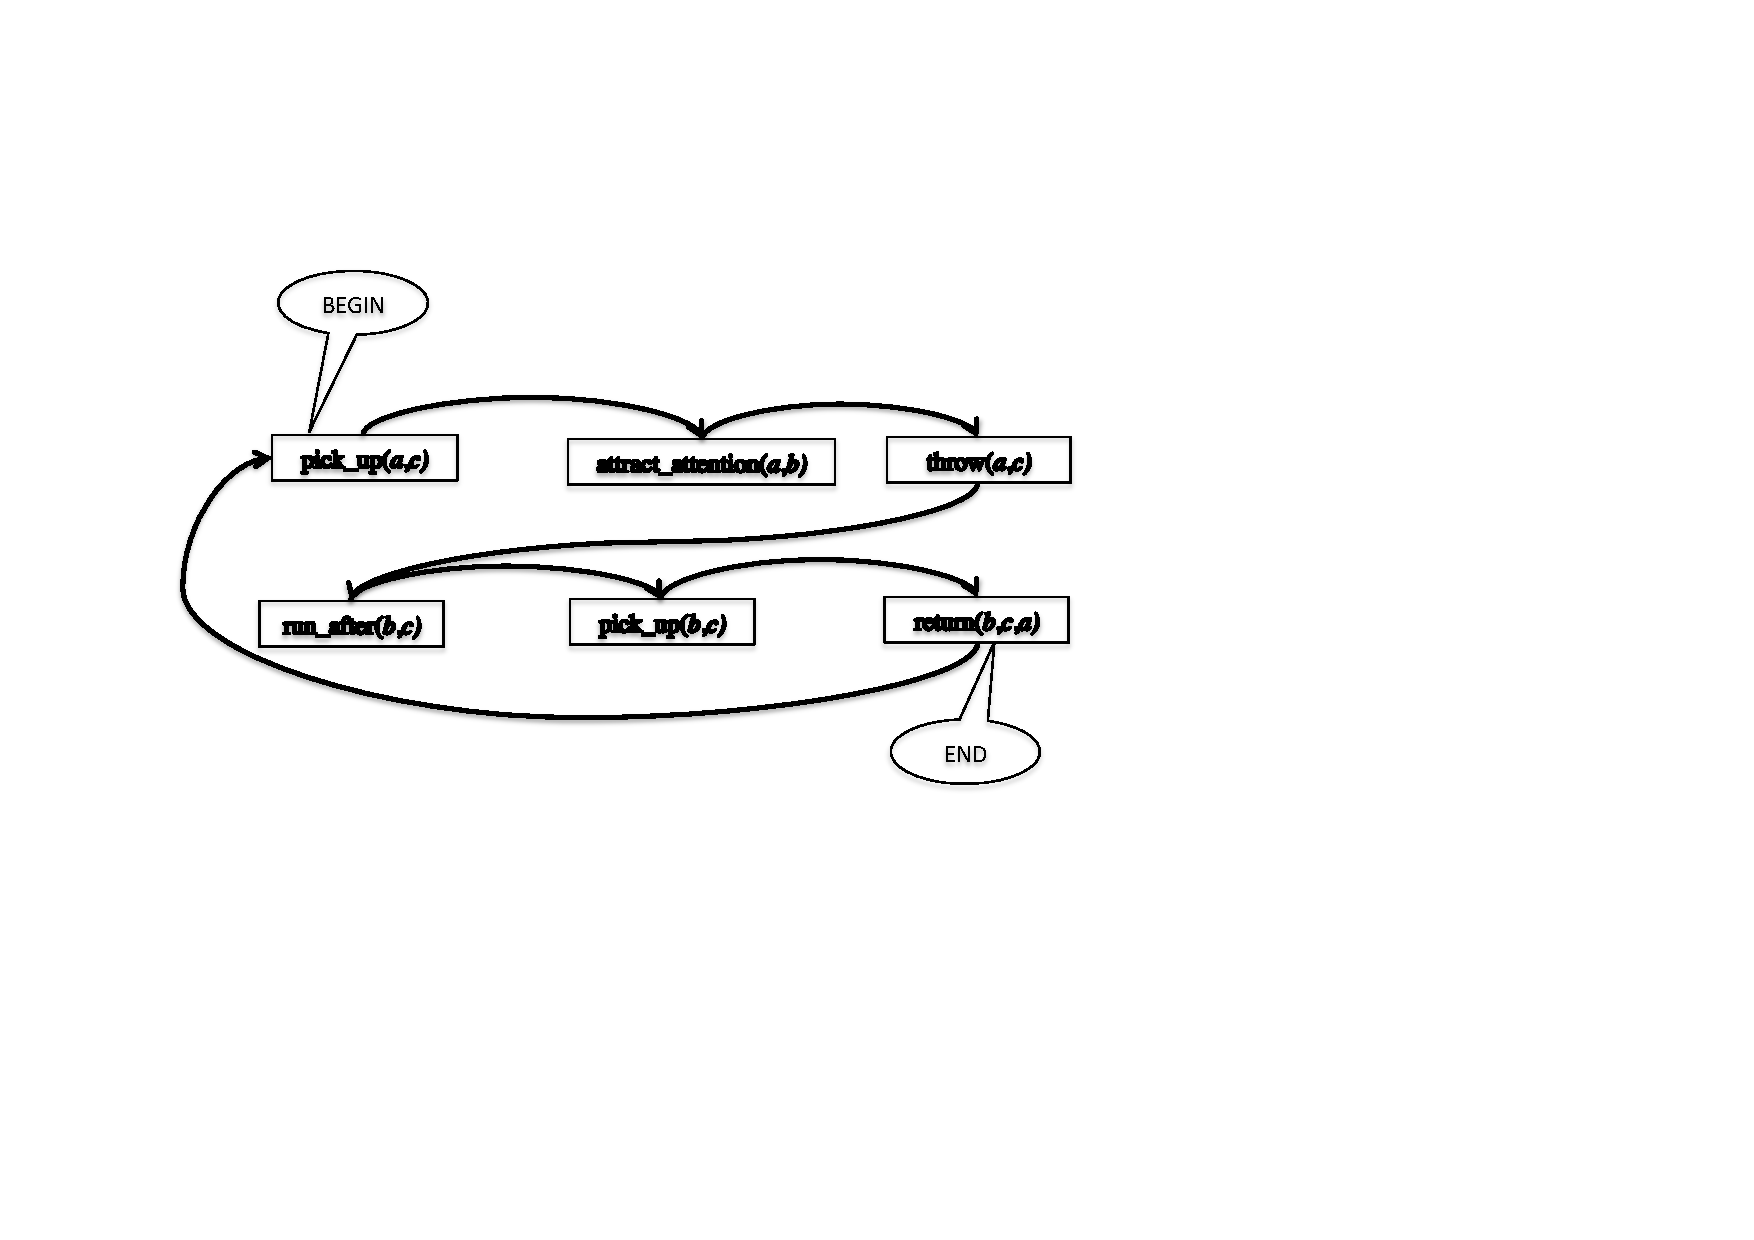
\includegraphics[width=6in]{fetch}

\hspace*{-4em}\begin{tikzpicture}[
  play/.style={rectangle, fill=Lamentation5, draw=Lamentation1, text=white, text depth=0.25ex, text height=1.5ex}
  ]

\node [play, pin=above:\textbf{Begin}] (p1) {pick\_up($a,c$)};
\node [play, right=of p1] (p2) {attract\_attention($a,b$)};
\node [play, right=of p2] (p3) {throw($a,c$)};
\node [play, below=1.5 of p1] (p4) {run\_after($b,c$)};
\node [play, right=of p4] (p5) {pick\_up($b,c$)};
\node [play, right=of p5, pin=below:\textbf{End}] (p6) {return($b,c,a$)};

\path [-{Stealth[]}, thick] 
(p1) edge [bend left] (p2)
(p2) edge [bend left] (p3)
(p3) edge [out=240, in=60] (p4)
(p4) edge [bend left] (p5)
(p5) edge [bend left] (p6)
(p6) edge [out=210, in=190, looseness=1.7] (p1);  
\end{tikzpicture}


\caption{play\_fetch($a$,$b$,$c$)}
\label{fig:fetch}
\end{figure}




   

In an important series of papers including
\cite{Fernando2004,Fernando2006,Fernando2008,Fernando2009,Fernando2011,Fernando2015}, Fernando introduces a finite state
approach to event analysis where events are analyzed in terms of
finite state automata something like what we have represented in
Figure~\ref{fig:fetch-fs}.
\begin{figure} 

%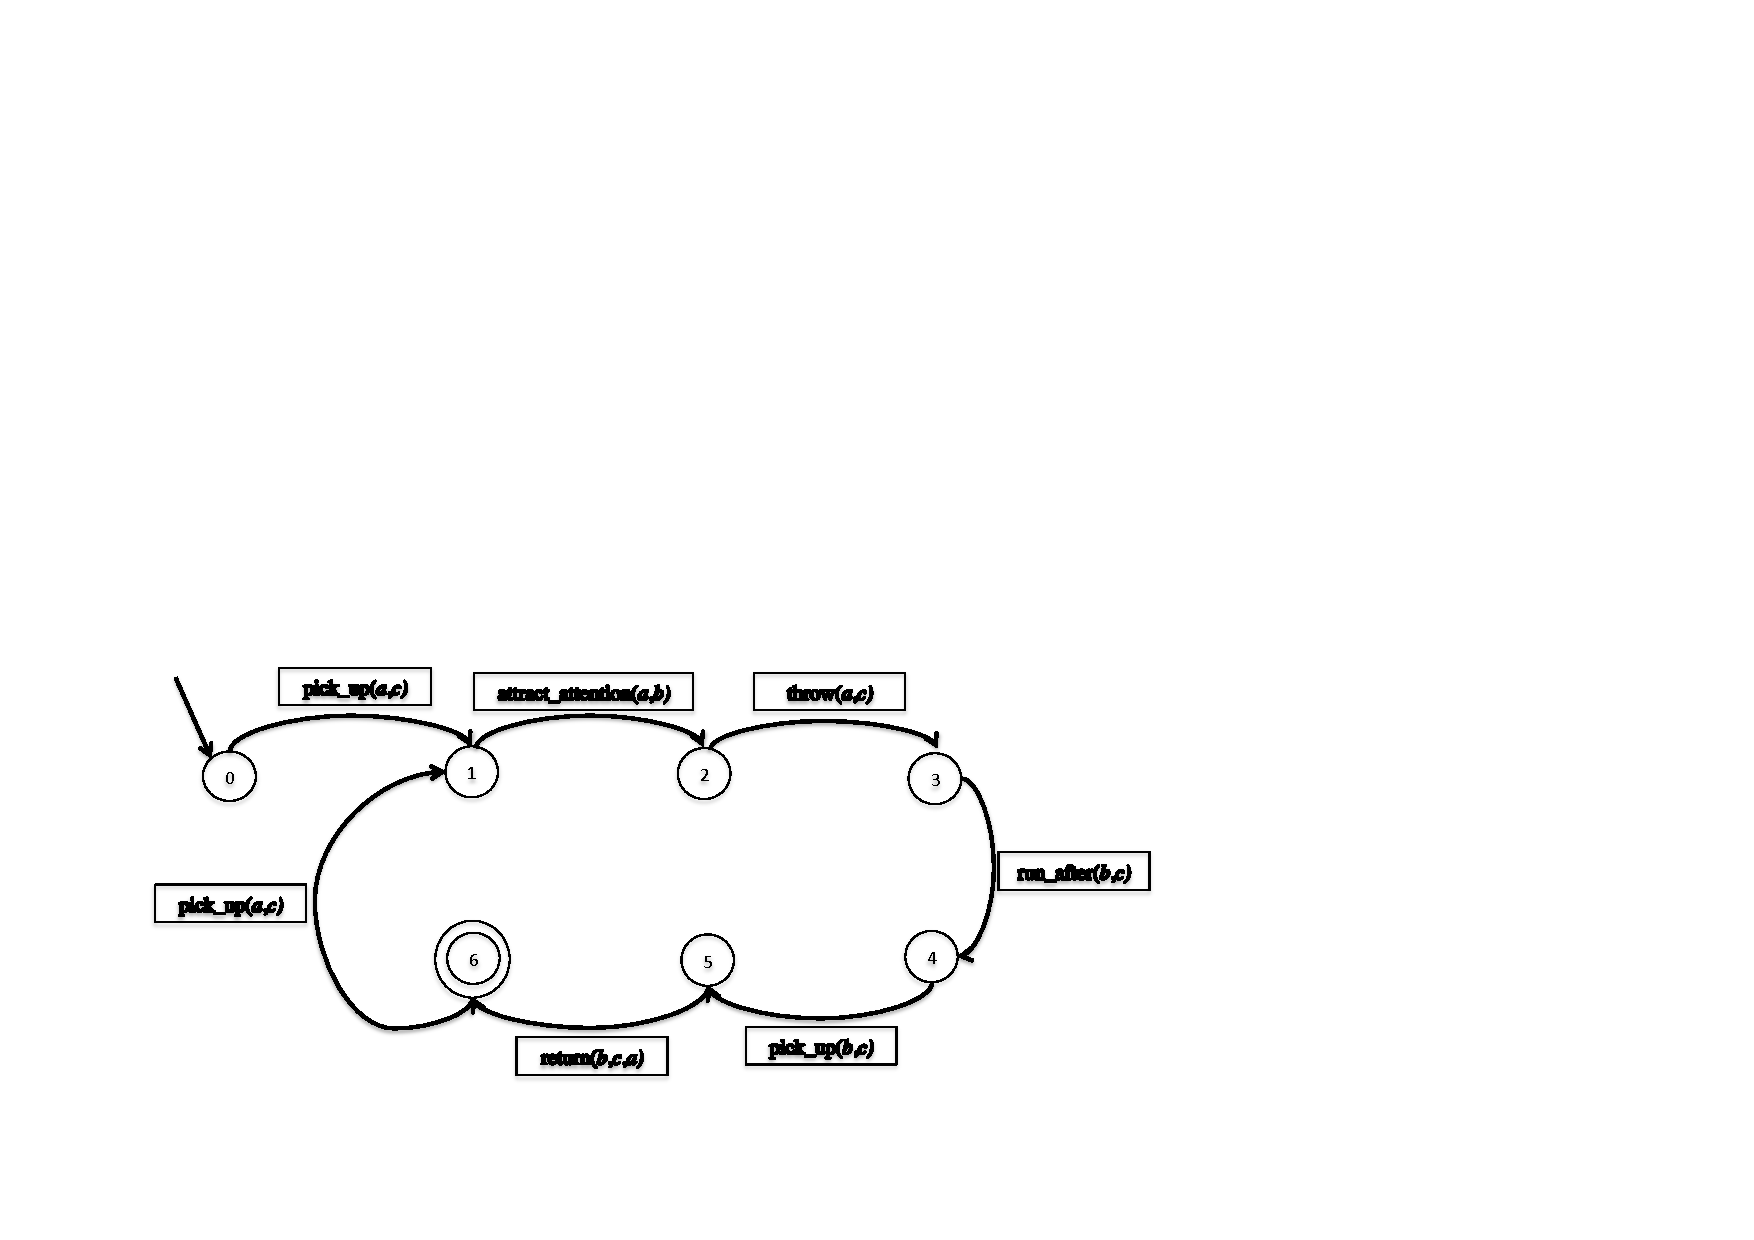
\includegraphics[width=6in]{fetch-fs}

\begin{tikzpicture}[
  node distance=3cm, 
  on grid,
  every state/.style={fill=Lamentation2},
  ]

\node [state, initial] (n0) {0};
\node [state] (n1) [right=of n0] {1};
\node [state] (n2) [right=of n1] {2};
\node [state] (n3) [right=of n2] {3};
\node [state] (n4) [below=of n3] {4};
\node [state] (n5) [left=of n4] {5};
\node [state, accepting] (n6) [left=of n5] {6};

\path [-{Stealth[]}, thick] 
(n0) edge [bend left] node [above] {pick\_up($a,c$)} (n1)
(n1) edge [bend left] node [above] {attract\_attention($a,b$)} (n2)
(n2) edge [bend left] node [above] {throw($a,c$)} (n3)
(n3) edge [bend left] node [right] {run\_after($b,c$)} (n4)
(n4) edge [bend left] node [below] {pick\_up($b,c$)} (n5)
(n5) edge [bend left] node [below] {return($b,c,a$)} (n6)
(n6) edge [bend left] node [left] {pick\_up($a,c$)} (n1);
\end{tikzpicture}


\caption{play\_fetch($a$,$b$,$c$) as a finite state machine}
\label{fig:fetch-fs}
\end{figure}  
Such an automaton will recognize a string of
sub-events.  The idea is that our perception of complex events can be seen as strings of
punctual observations similar to the kind of sampling we are
familiar with from audio technology and digitization processing in
speech recognition.  Thus events can be analyzed as strings of smaller
events.  % What we mean by a string is made precise in
% Appendix~\ref{sec:regular}.
Any object of any type can be part of a
string.  Any two objects (including strings themselves), $s_1$ and $s_2$, can be
\textit{concatenated} to form a string $s_1s_2$.  An
important property of concatenation is \textit{associativity}, that is
if we concatenate $s_1$ with $s_2$ and then concatenate the result
with $s_3$ we get the same string that we would obtain by
concatenating $s_2$ with $s_3$ and then concatenating $s_1$ with the
result.  In symbols: $(s_1s_2)s_3 =
s_1(s_2s_3)$.  For this reason we normally write
$s_1s_2s_3$ (without the parentheses).  Following Fernando we will use these strings to
give us our notion of temporal order.

If $a_1,a_2,\ldots,a_n$ are objects we will normally represent the
string of these objects as $a_1a_2\ldots a_n$.  Where confusion might
arise from this notation we use $\mathrm{str}(a_1a_2\ldots a_n)$.
This latter notation will be particularly useful when distinguishing a
single object, $a$, from a unit string containing this object
$\mathrm{str}(a)$.  Although we will present strings in this way, we will model them as
records \label{pg:stringsasrecords} with distinguished labels related to the natural numbers, 
t$_0$, t$_1$, \ldots (`t' for ``time'').  The field labelled t$_n$
will correspond to the $n+1$th place in the string.  Thus a string of
objects $a_1a_2a_3$
will be the record in \nexteg{}.
\begin{ex} 
\record{\field{t$_0$}{$a_1$} \\
        \field{t$_1$}{$a_2$} \\
        \field{t$_2$}{$a_3$}} 
\end{ex} 
The concatenation of \preveg{} with the string $a_4$, that is, \nexteg{a}, will
be \nexteg{b}.
\begin{ex} 
\begin{subex} 
 
\item \record{\field{t$_0$}{$a_4$}} 
 
\item  \record{\field{t$_0$}{$a_1$} \\
        \field{t$_1$}{$a_2$} \\
        \field{t$_2$}{$a_3$} \\
        \field{t$_3$}{$a_4$}}
 
\end{subex} 
   
\end{ex}

\begin{shaded}
Strings can be introduced into a type system with record types by the
definition in \nexteg{} (repeated in Appendix~\ref{app:strings})
\begin{ex} 
A system of complex types  \textbf{TYPE}$_C$ = $\langle${\bf Type}, {\bf BType},
$\langle$\textbf{PType}, {\bf Pred}, \textbf{ArgIndices}, {\it
  Arity\/}$\rangle$, $\langle A,F\rangle$$\rangle$ with record types
based on $\langle\mathcal{L}, \mathbf{RType}\rangle$ \textit{has strings}
if
\begin{enumerate} 
 
\item for each natural number $i$, t$_i\in\mathcal{L}$
 
\item \textit{String} $\in$ \textbf{BType}

\item $\emptyset:_{\mathbf{TYPE}_C}$ \textit{String}

\item if $T \in$ \textbf{Type} and $a:_{\mathbf{TYPE}_C}T$ then
  $\{\langle\text{t}_0,a\rangle\} : \textit{String}$

\item if $s$ :$_{\mathbf{TYPE}_C}$ \textit{String}, t$_n\in\mathrm{labels}(s)$ such that
  there is no $i>n$ where t$_i\in\mathrm{labels}(s)$, $T \in$ \textbf{Type}
  and $a:_{\mathbf{TYPE}_C}T$ then $s\cup\{\langle \mathrm{t}_{n+1},a\rangle\}$ :$_{\mathbf{TYPE}_C}$
  \textit{String}

\item Nothing is of type \textit{String} except as required above.
 
\end{enumerate}
\label{ex:string-sys} 
\end{ex} 
\preveg{}, clause~1 ensures that the labels $t_i$ are among the labels
available for forming record types.  Clause~2 introduces a basic type
\textit{String}.  Clause~3 says the empty set (also known as the empty
record and empty string) is a string. Clause~4 says that if you have
an object, $a$, of some type then you can form a unit string
containing $a$.  That is the record
\smallrecord{\field{t$_0$}{$a$}}. Note that we always start with the
label `t$_0$'. Clause~5 says that we can always create a new string
from a string $s$ by adding an additional object to the end of it,
using a label `t$_{n+1}$' where $n$ is the highest number such that
$\text{t}_n\in\mathrm{labels}(s)$.  Clause~6 is an exclusion clause.
Clauses~3--6 constitute an inductive definition of the set of
witnesses of the type \textit{String}.

In our informal proof theoretic notation this can be characterized by
giving an inductive definition as in \nexteg{}.
\begin{ex} 
For $\Gamma$ a system of complex types with record types based on
$\langle\mathcal{L},\mathbf{RType}\rangle$ and strings
\begin{subex} 
 
\item \begin{prooftree}
\infer0[$i\in\textit{Nat}$]{\text{t}_i\in\mathcal{L}} 
\end{prooftree} 

\item \begin{prooftree}
\infer0{\Gamma\vdash\textit{String}\in\textbf{BType}}
\end{prooftree}

\item \begin{prooftree}
\infer0{\Gamma\vdash\emptyset:\textit{String}}
\end{prooftree}

\item \begin{prooftree}
\hypo{\Gamma\vdash a:T}
\infer1{\Gamma\vdash\{\langle\text{t}_0,a\rangle\}:\textit{String}}
\end{prooftree} 

\item \begin{prooftree}
\hypo{\Gamma\vdash s:\textit{String}}
\hypo{\Gamma\vdash a:T}
\hypo{\{\text{t}_0,\ldots,\text{t}_n\}=\mathrm{labels}(s)}
\infer3[$n\geq 0$]{\Gamma\vdash
  s\cup\{\langle\text{t}_{n+1},a\rangle\}:\textit{String}}
\end{prooftree}
 
\end{subex} 
   
\end{ex} 
    
\end{shaded} 
We will continue to
represent strings for convenience in the traditional way but modelling
strings as records will become important when following paths in
records down to elements in strings and any operations we define on
records will automatically generalize to strings.  We will use
$\varepsilon$ to represent the empty string (that is, the empty set). We will use $s[n]$ to represent
the $n$th element in a string $s$ (where the first element in the
string is $s[0]$).  In terms of the record notation
this is just a convenient abbreviation for $s$.t$_n$.

\label{pg:stringtype-notation}We will use $T^{=n}$, or, when there is no risk of confusion, simply
$T^n$, as the type of strings of length $n$ all of whose elements are
of type $T$. We will use $T^{\geq n}$ for the type of strings of
objects of type $T$ which have length greater than or equal to $n$.
In particular we will use $T^*$ (the Kleene star) for $T^{\geq0}$ and
$T^+$ (the Kleene plus) for $T^{\geq1}$.

\begin{shaded}
We can make this precise with the definition in \nexteg{} (repeated in
Appendix~\ref{app:strings})
\begin{ex} 
A system of complex types  \textbf{TYPE}$_C$ = $\langle${\bf Type}, {\bf BType},
$\langle$\textbf{PType}, {\bf Pred}, \textbf{ArgIndices}, {\it
  Arity\/}$\rangle$, $\langle A,F\rangle$$\rangle$ with strings has
\textit{length determining string types} if
\begin{enumerate} 
 
\item for any $T\in\textbf{Type}$ and $n$ a natural number, the string
  types $T^{=n}$,
  $T^{\leq n}$, $T^{\geq n}\in\textbf{Type}$ 
 
\item $s:_{\mathbf{TYPE}_C}T^{=n}\ (T^{\leq n}, T^{\geq n})$ iff
  $s:_{\mathbf{TYPE}_C}\textit{String}$, for all $i$, $0\leq
  i<\mathrm{length}(s)$, $s[i]:_{\mathbf{TYPE_C}}T$ and $\mathrm{length}(s) =
  (\leq,\geq)\ n$ 
 
\end{enumerate}
\label{ex:ldstringtypes} 
\end{ex} 

In our informal proof theoretic notation this can be expressed as
\nexteg{}.
\begin{ex} 
For $\Gamma$ a system of complex types with strings and length
determining string types:
\begin{subex} 
 
\item \begin{prooftree}
\hypo{\Gamma\vdash T\in\textbf{Type}}
\infer1[$n\in\textit{Nat}$]{\Gamma\vdash T^{=n}\in\textbf{Type}}
\end{prooftree}
\hspace*{2em}
\begin{prooftree}
\hypo{\Gamma\vdash T\in\textbf{Type}}
\infer1[$n\in\textit{Nat}$]{\Gamma\vdash T^{\leq n}\in\textbf{Type}}
\end{prooftree}
\hspace*{2em}
\begin{prooftree}
\hypo{\Gamma\vdash T\in\textbf{Type}}
\infer1[$n\in\textit{Nat}$]{\Gamma\vdash T^{\geq n}\in\textbf{Type}}
\end{prooftree}
 
 
\item  \begin{prooftree}
\hypo{\Gamma\vdash s:\textit{String}}
\hypo{\mathrm{length}(s)=n}
\hypo{[i<n]}
\ellipsis{}{\Gamma\vdash s[i]:T}
\infer3{\Gamma\vdash s:T^{=n}}
\end{prooftree}
\hspace*{2em}
\begin{prooftree}
\hypo{\Gamma\vdash s:\textit{String}}
\hypo{\mathrm{length}(s)\leq n}
\hypo{[i<\mathrm{length}(s)]}
\ellipsis{}{\Gamma\vdash s[i]:T}
\infer3{\Gamma\vdash s:T^{\leq n}}
\end{prooftree}
\hspace*{2em}
\begin{prooftree}
\hypo{\Gamma\vdash s:\textit{String}}
\hypo{\mathrm{length}(s)\geq n}
\hypo{[i<\mathrm{length}(s)]}
\ellipsis{}{\Gamma\vdash s[i]:T}
\infer3{\Gamma\vdash s:T^{\geq n}}
\end{prooftree} 
\end{subex} 
  
\end{ex}
\preveg{a} introduces the string types and \preveg{b} specifies
witness conditions for the types. 
  
  
\end{shaded}    

Next we introduce concatenation types.  For any
two types, $T_1$ and $T_2$, we can form the type ${T_1}^{\frown}T_2$.
This is the type of strings $ab$ where $a:T_1$ and $b:T_2$.
The concatenation operation on types (just like that on objects) is
associative so we do not use parentheses when more than one type is
involved, e.g. ${T_1}^{\frown}{T_2}^{\frown}T_3$.

\begin{shaded}
This can be made precise as \nexteg{}, repeated in
Appendix~\ref{app:strings}.
\begin{ex} 
A system of complex types  \textbf{TYPE}$_C$ = $\langle${\bf Type}, {\bf BType},
$\langle$\textbf{PType}, {\bf Pred}, \textbf{ArgIndices}, {\it
  Arity\/}$\rangle$, $\langle A,F\rangle$$\rangle$ with strings and
length determining string types has \textit{concatenation types}
if
\begin{enumerate} 
 
\item if $T_1$, $T_2\in\textbf{Type}$ then the string type $T_1^\frown T_2\in\textbf{Type}$ 
 
\item $s:_{\mathbf{TYPE}_C}T_1^\frown T_2$ iff there are $s_1$ and
  $s_2$ such that
\begin{enumerate} 
 
\item $s_1s_2=s$ 
 
\item $s_1:_{\mathbf{TYPE}_C}T_1$ if $T_1$ is a string type, otherwise
  $s_1:_{\mathbf{TYPE}_C}{T_1}^{=1}$

\item $s_2:_{\mathbf{TYPE}_C}T_2$ if $T_2$ is a string type, otherwise
  $s_2:_{\mathbf{TYPE}_C}{T_2}^{=1}$  
 
\end{enumerate} 
   
 
\end{enumerate} 
\label{ex:concatenation-types} 
\end{ex}
Clause~1 introduces concatenation types, $T_1^\frown T_2$, and clause~2 says that
witnesses for concatenative types must be the concatenation of two
strings which are of the types $T_1$ and $T_2$ resepctively if they
are string types of if they are not they must be of the type of
singleton strings whose only element is of type $T_1$ or $T_2$
respectively.  

We can express this in our informal proof theoretic notation as
\nexteg{}.
\begin{ex} 
For $\Gamma$ a system of complex types with strings, length
determining string types and concatenative string types
\begin{subex} 
 
\item \begin{prooftree}
\hypo{\Gamma\vdash T_1\in\textbf{Type}}
\hypo{\Gamma\vdash T_2\in\textbf{Type}}
\infer2{\Gamma\vdash {T_1}^\frown T_2\in\textbf{Type}}
\end{prooftree} 
 
\item \begin{prooftree}
\hypo{\Gamma\vdash s_1:T_1'}
\hypo{\Gamma\vdash s_2:T_2'}
\infer2[$T_i'=T_i$ if $T_i$ is a string type; otherwise
$T_i'=T_i^{=1}$]{\Gamma\vdash s_1s_2:T_1^\frown T_2}
\end{prooftree} 
 
\end{subex} 
   
\end{ex} 
\preveg{a} introduces concatenative types, $T_1^\frown T_2$,  and
\preveg{b} tells us that witnesses for these types are concatenations
of two strings, $s_1$ and $s_2$, where $s_1:T_1$ (or $s_1:T_1^{=1}$ if
$T_1$ is not a string type) and similarly for $s_2$ and $T_2$. 

To \preveg{} we can add \nexteg{} to express the associativity of
`$^\frown$'.
\begin{ex} 
\begin{prooftree}
\hypo{\Gamma\vdash (T_1^\frown T_2)^\frown T_3\in\textbf{Type}}
\hypo{\Gamma\vdash T_1^\frown(T_2^\frown T_3)\in\textbf{Type}}
\infer2{\Gamma\vdash(T_1^\frown T_2)^\frown T_3 =
  T_1^\frown(T_2^\frown T_3)\in\textbf{Type}}
\end{prooftree}
\end{ex} 
   
  

\end{shaded}

While strings as we have defined them are useful for modelling events
in terms of strings of subevents, it is not the case that all strings
of events
can be considered as occurring events.  Consider a case where we have
to events as characterized in \nexteg{}.
\begin{ex} 
\begin{subex} 
 
\item $e_1:T_1$ 
 
\item $e_2:T_2$ 
 
\end{subex} 
   
\end{ex} 
The type theory as we have defined it will yield both
juedgements in \nexteg{}.
\begin{ex} 
\begin{subex} 
 
\item $e_1e_2:T_1^{\frown}T_2$ 
 
\item $e_2e_1:T_2^{\frown}T_1$ 
 
\end{subex} 
   
\end{ex} 
However, if we are using event strings to model temporal ordering it
cannot be the case that both $e_1e_2$ and $e_2e_1$ both model
occurring events even though they are both strings of events.  That
is, if $e_1$ temporally precedes $e_2$ then $e_2$ cannot temporally
precede $e_1$  and \textit{vice versa}.  This has to do with the fact
that a particular event can only happen once.  It is, of course,
possible to have different events of the same types occurring in the
reverse order as in \nexteg{}.
\begin{ex} 
\begin{subex} 
 
\item $e_1e_2:T_1^{\frown}T_2$ 
 
\item $e_3e_4:T_2^{\frown}T_1$ 
 
\end{subex} 
   
\end{ex} 
One way to distinguish those strings which correspond to occurring
events from those which do not is to introduce a type \textit{Occur}
such that if $e_1e_2:\textit{Occur}$ then $e_2e_1\not:\textit{Occur}$.
Below we will use records to model the simultaneous occurrence of
events.  We can do this by allowing records to be witnesses for
\textit{Occur} and requiring that if $r:\textit{Occur}$ and
$\ell_1,\ell_2\in\mathrm{labels}(r)$ then
$r.\ell_1r.\ell_2\not:\textit{Occur}$.  We will not develop this idea
further here but assume it in the background.  

Let us return to Kim watching the boy, $a$, playing fetch with the
dog, $b$, using the stick, $c$. % over a time interval $t$
She
perceives the event as being of type play\_fetch($a$,$b$,$c$).
But what does it mean to be an event of this type?  Given our
concatenation types we can build a type which corresponds to most of
what we have sketched in Figure~\ref{fig:fetch}, namely \nexteg{}.
% (again ignoring time for the sake of simplification).
\begin{ex} 
pick\_up($a$,$c$)$^{\frown}$attract\_attention($a$,$b$)$^{\frown}$throw($a$,$c$)$^{\frown}$run\_after($b$,$c$)$^{\frown}$pick\_up($b$,$c$)$^{\frown}$\\
\hspace*{2em}return($b$,$c$,$a$) 
\end{ex} 
\preveg{} is a type corresponding to everything we have represented in
Figure~\ref{fig:fetch} except for the arrow which loops back from the
end state to the start state.    In order to get the loop into the event
type we will use a Kleene-+ type.  % In
% standard notations for strings $s^+$ stands for a string consisting of
% one or more occurrences of $s$.\footnote{This notation was introduced
%   by the mathematician Stephen Kleene.}
% We will adopt this into types
% by saying that for any type $T$ there is also a type $T^+$ which is
% the type of strings of objects of type $T$ containing one or more
% members.  (See Appendix~\ref{sec:regular} for a more precise
% definition.)
The type \nexteg{} will, then,
give us a type corresponding to the complete Figure~\ref{fig:fetch}
since it will be the type consisting of strings of one or more events
of the type \preveg{}.
\begin{ex} 
(pick\_up($a$,$c$)$^{\frown}$attract\_attention($a$,$b$)$^{\frown}$throw($a$,$c$)$^{\frown}$run\_after($b$,$c$)$^{\frown}$pick\_up($b$,$c$)$^{\frown}$
\\ \hspace*{2em}return($b$,$c$,$a$))$^+$ 
\end{ex}


% In \preveg{} we simplified the string type by excluding time.  Now we
% will consider what is needed to put time back in.  Each of the
% subevents represented there is associated with a time interval, a
% different time interval for each subevent.  The type for time
% intervals, which we will abbreviate as \textit{TimeInt} is \nexteg{}\label{pg:TimeInt}.
% \begin{ex} 
% \record{\tfield{start}{\textit{Time}} \\
%         \tfield{end}{\textit{Time}} \\
%         \tfield{c$_<$}{start$<$end}}
% \end{ex} 
% where \textit{Time} is the type of time points and $<$ is the relation
% ``earlier than'' defined on the witnesses of this type.\footnote{We
%   use the infix notation $t_1<t_2$ rather than the official notation
%   $<(t_1,t_2)$.}  In order to get time intervals associated with each
% subevent we will treat the subevent types as record types rather than
% ptypes.  Thus as a first step towards characterizing the right type we
% have \nexteg{}.
% \begin{ex} 
% \smallrecord{\smalltfield{e-time}{\textit{TimeInt}} \\
%              \smalltfield{c$_{\mathrm{pick\_up}}$}{pick\_up($a$,$c$,e-time)}}$^{\frown}$\smallrecord{\smalltfield{e-time}{\textit{TimeInt}}
%              \\
%                   \smalltfield{c$_{\mathrm{attract\_attention}}$}{attract\_attention($a$,$b$,e-time)}}$^{\frown}$

% \medskip
% \smallrecord{\smalltfield{e-time}{\textit{TimeInt}} \\
%              \smalltfield{c$_{\mathrm{throw}}$}{throw($a$,$c$,e-time)}}$^{\frown}$\smallrecord{\smalltfield{e-time}{\textit{TimeInt}} \\
%              \smalltfield{c$_{\mathrm{run\_after}}$}{run\_after($b$,$c$,e-time)}}$^{\frown}$

% \medskip
% \smallrecord{\smalltfield{e-time}{\textit{TimeInt}} \\
%              \smalltfield{c$_{\mathrm{pick\_up}}$}{pick\_up($b$,$c$,e-time)}}$^{\frown}$\smallrecord{\smalltfield{e-time}{\textit{TimeInt}} \\
%              \smalltfield{c$_{\mathrm{return}}$}{return($b$,$c$,$a$,e-time) }}
% \end{ex}

% This will get us a time interval for each subevent but it does not
% require any relationship between the time intervals of the different
% subevents whereas, of course, each subevent should occur at a later
% time than the previous one.  In order to achieve this we will
% introduce a more restricted notion of type concatenation especially
% for record types which have a field
% \smallrecord{\smalltfield{e-time}{\textit{TimeInt}}} as in \nexteg{}.
% \begin{ex}
% \begin{enumerate} 
% \item If $T_1$ and $T_2$ are subtypes of
% \smallrecord{\smalltfield{e-time}{\textit{TimeInt}}}$^+$ then
% $T_1^{\frown_<}T_2$ is a type. 

% \item $a:T_1^{\frown_<}T_2$ iff $a=a_1^{\frown}a_2$, $a_1:T_1$, $a_2:T_2$ and
%   last($a_1$).e-time.end$<$first($a_2$).e-time.start
% \end{enumerate}
% \end{ex} 
% Here first($s$) and last($s$) pick out the first and last elements
% respectively of the string $s$.  We need to make a similar adjustment
% to the Kleene-+ type constructor.
% \begin{ex} 
% \begin{enumerate} 
 
% \item If $T$ is a subtype of
%   \smallrecord{\smalltfield{e-time}{\textit{TimeInt}}} then $T^{+_<}$
%   is a type
 
% \item $a:T^{+_<}$ iff $a=x_1^\frown\!\ldots^\frown\!x_n$, $n>0$ and
%   for $i$, $j$, $1\leq
% i<j\leq n$, $x_i:T$, $x_j:T$ and $x_i^{\frown}x_j:T^{\frown_<}T$ 
 
% \end{enumerate} 
   
% \end{ex} 

% [The details of temporal concatenation above should be included in the
% appendix.]

We will complicate \preveg{} slightly by substituting record types for
the ptypes as in \nexteg{}.  We do this because we
will want to allow for things happening simultaneously and record
types will give us a straightforward way of allowing this.
\begin{ex} 
(\smallrecord{\smalltfield{e}{pick\_up($a$,$c$)}}$^{\frown}$\smallrecord{\smalltfield{e}{attract\_attention($a$,$b$)}}$^{\frown}$\smallrecord{\smalltfield{e}{throw($a$,$c$)}}$^{\frown}$\smallrecord{\smalltfield{e}{run\_after($b$,$c$)}}$^{\frown}$\\
\hspace*{2em}\smallrecord{\smalltfield{e}{pick\_up($b$,$c$)}}$^{\frown}$\smallrecord{\smalltfield{e}{return($b$,$c$,$a$)}})$^+$ 
\label{eg:fetch-type}
\end{ex}
The label `e' (``event'') occurs in each of the elements of the string
type.  In this case we will say that `e' labels a \textit{dimension}
of events of this type.  The `e'-dimension can be thought of as the
dimension which characterizes what is happening at each stage of the
event.  % If you want to think geometrically, you can think of the
% event-string as being located in a space of event types (that is, the ptypes).

% So now we can represent the event type for playing fetch as \nexteg{}.
% \begin{ex} 
% (\smallrecord{\smalltfield{e-time}{\textit{TimeInt}} \\
%              \smalltfield{c$_{\mathrm{pick\_up}}$}{pick\_up($a$,$c$,e-time)}}$^{\frown_<}$\smallrecord{\smalltfield{e-time}{\textit{TimeInt}}
%              \\
%                   \smalltfield{c$_{\mathrm{attract\_attention}}$}{attract\_attention($a$,$b$,e-time)}}$^{\frown_<}$

% \medskip
% \smallrecord{\smalltfield{e-time}{\textit{TimeInt}} \\
%              \smalltfield{c$_{\mathrm{throw}}$}{throw($a$,$c$,e-time)}}$^{\frown_<}$\smallrecord{\smalltfield{e-time}{\textit{TimeInt}} \\
%              \smalltfield{c$_{\mathrm{run\_after}}$}{run\_after($b$,$c$,e-time)}}$^{\frown_<}$

% \medskip
% \smallrecord{\smalltfield{e-time}{\textit{TimeInt}} \\
%              \smalltfield{c$_{\mathrm{pick\_up}}$}{pick\_up($b$,$c$,e-time)}}$^{\frown_<}$\smallrecord{\smalltfield{e-time}{\textit{TimeInt}} \\
%              \smalltfield{c$_{\mathrm{return}}$}{return($b$,$c$,$a$,e-time) }})$^{+_<}$
% \end{ex}


\section{Doing things with types}
\label{sec:typeacts}

\subsection{Type acts}

The boy and the dog have to coordinate and interact in order to create an
event of the game of fetch.  This involves doing more with types than
just making judgements.  For example, when the dog observes the
situation in which the boy raises the stick, it may not be clear
to the dog whether this is part of a fetch-game situation or a
stick-beating situation.  The dog may be in a situation of
entertaining these two types as possibilities prior to making the
judgement that the situation is of the fetch type.  We will call this
act a query as opposed to a judgement.  Once the dog has made the
judgement that what it has observed so far is an initial segment of a
fetch type situation it has to make its own contribution in order to
realize the fetch type, that is, it has to run after the stick and
bring it back.  This involves the creation of a situation of a certain
type.  Thus creation acts are another kind of act related to types.
Creating objects of a given type often has a \textit{de se}
\citep[see, for example,][]{Perry1979,Lewis1979a,Ninan2010,Schlenker2011} aspect.  The dog
has to know that it itself must run after the stick in order to make
this a situation in which it and the boy are playing fetch.  There is
something akin to what Perry calls an essential indexical here,
though, of course, the dog does not have indexical linguistic
expressions. It is nevertheless part of the basic competence that an
agent needs in order to be able to coordinate its action with the rest
of the world that it has a primitive sense of self which is distinct
from being able to identify an object which has the same properties as
itself.  We will follow Lewis in modelling \textit{de se} in terms of
functional abstraction over the ``self''.  In our terms this will mean
that \textit{de se} type acts involve dependent types.

In standard type theory we have judgements such as $o:T$ ``$o$ is of type $T$'' 
and 
$T$ \textit{true} ``there is something of type $T$''.    We want to
enhance this notion of judgement by including a reference to the agent
$A$ which makes the judgement, giving judgements such as
$o:_AT$ ``agent $A$ judges that $o$ is of type $T$''
and 
$:_AT$ ``agent $A$ judges that there is some object of type $T$''. We will call
the first of these a \textit{specific} judgement and the second a
\textit{non-specific} judgement.  Such
judgements are one of the three kinds of acts represented in \nexteg{}
that we want to include
in our type act theory.
\begin{ex} 
\textit{Type Acts}
\begin{description}
\item[judgements] \mbox{}

\begin{description}
\item[\textit{specific}] $o:_A T$ ``agent $A$ judges object $o$ to be of type
  $T$''

\item[\textit{non-specific}] $:_A T$ ``agent $A$ judges that there is some
  object of type $T$''
\end{description}

\item[queries] \mbox{}
\begin{description}
\item[\textit{specific}] $o:_A T?$ ``agent $A$ wonders whether object $o$ is of type
  $T$''

\item[\textit{non-specific}] $:_A T?$ ``agent $A$ wonders whether there is some object of type
$T$''
\end{description}
\item[creations] \mbox{}
\begin{description}
\item[\textit{non-specific}] $:_A T!$ ``agent $A$ creates something of type
  $T$''
\end{description}
\end{description}

\end{ex} 
Note that creations only come in the non-specific variant.  You cannot
create an object which already exists.  

Creations are also limited in
that there are certain types which a given agent is not able to
realize as the main actor.  Consider for example the event type involved in the fetch
game of the dog running after the stick.  The human cannot be the main
creator of such
an event since it is the dog who is the actor.  The most the human can
do is wait until the dog has carried out the action
and we will count this as a creation type act.  This will become
important when we discuss coordination in the fetch-game below.  It is
actually important that the human makes this passive contribution to
the creation of the event of the dog running after the stick and does
not, for example, get the game confused by immediately throwing
another stick before the dog has had a chance to retrieve the first
stick.  There are other cases of event types which require a less
passive contribution from an agent other than the main actor.
Consider the type of event where the dog returns the stick to the
human.  The dog is clearly the main actor here but the human has also
a role to play in making the event realized.  For example, if the
human turns her back on the dog and ignores what is happening or runs
away, the event type will not be realized despite the dog's best
efforts.  Other event types, such as lifting a piano, involve more
equal collaboration between two or more agents, where it is not
intuitively clear that any one of the agents is the main actor.  So
when we say ``agent $A$ creates something of type $T$'' perhaps it
would be more accurate to phrase this as ``agent $A$ contributes to
the creation of something of type $T$'' where $A$'s contribution might
be as little as  not realizing any of the other types involved in the game until
$T$ has been realized.   
   
\textit{De se} type acts involve functions which have the agent in its
domain and return a type, that is, they are dependent types which,
given the agent, will yield a type.  We will say that agents are of
type \textit{Ind} and that the relevant dependent types, 
$\mathcal{T}$, are functions of type
  (\textit{Ind}$\rightarrow$\textit{Type}).  
We characterize \textit{de se} type acts in a way parallel to
\preveg{}, as given in \nexteg{}.
\begin{ex}
\textit{De Se Type Acts} 
\begin{description}
\item[\textit{judgements}] \mbox{}
\begin{description}
\item[\textit{specific}]  $o:_A \mathcal{T}(A)$ ``agent $A$ judges object $o$ to be of type
  $\mathcal{T}(A)$''
\item[\textit{non-specific}] $:_A \mathcal{T}(A)$ ``agent $A$ judges
  that there is some object of type $\mathcal{T}(A)$''
\end{description}

\item[\textit{queries}] \mbox{}
\begin{description}
\item[\textit{specific}] $o:_A \mathcal{T}(A)?$ ``agent $A$ wonders whether object $o$ is of type
  $\mathcal{T}(A)$''
\item[\textit{non-specific}] $:_A \mathcal{T}(A)?$ ``agent $A$ wonders whether there is some object of type
$\mathcal{T}(A)$''
\end{description}

\item[\textit{creations}] \mbox{}
\begin{description}
\item[\textit{non-specific}] $:_A \mathcal{T}(A)!$ ``agent $A$ creates
  something of type $\mathcal{T}(A)$''
\end{description}
\end{description} 
\end{ex} 

From the point of view of the type theory \textit{de se} type acts
seem more complex than non-\textit{de se} type acts since they involve
a dependent rather than a non-dependent type and a functional
application of that dependent type to the agent.  However, from a
cognitive perspective one might expect \textit{de se} type acts to be
more basic.  Agents which perform type acts using types directly
related to themselves are behaving egocentrically and one could regard
it as a more advanced level of abstraction to consider types which are
independent of the agent.  This seems a puzzling way in which our
notions of type seem in conflict with out intuitions about cognition.   

While these type acts are prelinguistic (we need them to account for
the dog's behaviour in the game of fetch), it seems
that they are the basis on which the notion of speech act
\citep[and much subsequent literature]{Austin1962,Searle1969} is built.  % Our notion of using types in
% query acts seems intuitively related to work on inquisitive semantics
% \citep{GroenendijkRoelofsen2012} where some propositions (in
% particular disjunctions) are regarded as inquisitive.  However, this
% will still allow us to make a distinction between questions and
% assertions in natural language as argued for by \cite{Ginzburg2012}.

\subsection{Making inferences about events}
What happens
when Kim perceives an event as being of the type (\ref{eg:fetch-type})?  She
makes a series of observations of events, assigning them to types in
the string type.  Note that the ptypes in each of the types can be
further broken down in a similar way.  This gives us a whole hierarchy
of perceived events which at some point have to bottom out in basic
perceptions which are not further analyzed.  In order to recognize an
event as being of this type Kim does not need to perceive a string of
events corresponding to each of the types in the string types.  She
may, for example, observe the boy waving the stick to attract the
dog's attention, get distracted by a bird flying overhead for a while,
and then return to the fetch event at the point where the dog is
running back to the boy with the stick.  This still enables her to
perceive the event as an event of fetch playing because she has seen
such events before and learned that such events are of the string type in (\ref{eg:fetch-type}).  It suffices for her to observe enough of the elements in
the string to distinguish the event from other event types she may
have available in her knowledge resources.  Suppose, for example, that
she has just two event string types available that begin with the picking
up of a stick by a human in the company of a dog.  One is (\ref{eg:fetch-type}).
The other is one that leads to the human beating the dog with the
stick.  If she only observes the picking up of the stick she cannot be
sure whether what she is observing is a game of fetch or a beating.
However, as soon as she observes something in the event string which
belongs only to the fetch type she can reasonably conclude
that she is observing an event of the fetch type.  She may, of course,
be wrong.  She may be observing an event of a type which she does not
yet have available in her resource of event types, in which case she
will need to learn about the new event type and add it to her
resources.  However, given the resources at her disposal she can make
a prediction about the nature of the rest of the event.  One could
model her prediction making ability in terms of a function which maps
a situation (modelled as a record) to a type of predicted situation,
for example \nexteg{}.
\begin{ex} 
$\lambda r$:\smallrecord{\smalltfield{x}{\textit{Ind}} \\
                         \smalltfield{c$_{\mathrm{human}}$}{human(x)}
                         \\
                         \smalltfield{y}{\textit{Ind}} \\
                         \smalltfield{c$_{\mathrm{dog}}$}{dog(y)} \\
                         \smalltfield{z}{\textit{Ind}} \\
                         \smalltfield{c$_{\mathrm{stick}}$}{stick(z)}
                         \\
                         \smalltfield{e}{\smallrecord{
             \smalltfield{e}{pick\_up(x,z)}}$^{\frown}$\smallrecord{
                  \smalltfield{e}{attract\_attention(x,y)}}}} .
            \\*[.75\baselineskip]
\hspace*{4em}\smallrecord{\smalltfield{e}{play\_fetch($r$.x,$r$.y,$r$.z)}
\\
\smalltfield{c$_{\mathrm{init}}$}{init($r$.e,e)}}
\label{ex:ev-predict-fun}
\end{ex} 
% \begin{ex} 
% $\lambda r$:\smallrecord{\smalltfield{x}{\textit{Ind}} \\
%                          \smalltfield{c$_{\mathrm{human}}$}{human(x)}
%                          \\
%                          \smalltfield{y}{\textit{Ind}} \\
%                          \smalltfield{c$_{\mathrm{dog}}$}{dog(y)} \\
%                          \smalltfield{z}{\textit{Ind}} \\
%                          \smalltfield{c$_{\mathrm{stick}}$}{stick(z)}
%                          \\
%                          \smalltfield{e-time}{\textit{TimeInt}} \\
%                          \smalltfield{e}{\smallrecord{\smalltfield{e-time}{\textit{TimeInt}}
%                              \\
% \smalltfield{c$_{\leq}$}{$\Uparrow$e-time.start$\leq$e-time.start} \\
%              \smalltfield{c$_{\mathrm{pick\_up}}$}{pick\_up($\Uparrow$x,$\Uparrow$z,e-time)}}$^{\frown_<}$\smallrecord{\smalltfield{e-time}{\textit{TimeInt}}
%              \\
% \smalltfield{c$_{\leq}$}{e-time.start$\leq\Uparrow$e-time.start} \\
%                   \smalltfield{c$_{\mathrm{attract\_attention}}$}{attract\_attention($\Uparrow$x,$\Uparrow$y,e-time)}}}}
%             \\*[.75\baselineskip]
% \hspace*{4em}(\smallrecord{\smalltfield{e-time}{\textit{TimeInt}} \\
%                            \smalltfield{c$_{\leq}$}{$r$.e-time.start$\leq$e-time.start} \\
%                            \smalltfield{e}{play\_fetch($r$.x,$r$.y,$r$.z,e-time)}})
% \label{ex:ev-predict-fun}
% \end{ex}

Here the predicate `init' has arity
$\langle$\textit{String}, \textit{String}$\rangle$.  The type init($s_1$,$s_2$) is
non-empty just in case $s_1$ is an initial substring of $s_2$.  

\begin{shaded}
We
achieve this by the definition in \nexteg{}, repeated in Appendix~\ref{app:strings}.
\begin{ex}
If $s_1$ is a string of length $n$ and $s_2$ is a string of any
length, then $s$ : init($s_1$,$s_2$) iff the length of $s_2$ is
greater than or equal to $n$ and for each $i$, $0\leq i<n$,
$s_1[i]=s_2[i]$ and $s=s_2$.
\end{ex}
That is, if the initial substring condition holds then the second
argument to the predicate (and nothing else) is of the ptype.
\end{shaded}

% Here a `$\Uparrow$' prefixed to a path-name consisting of labels such
% as `e-time.start' or `x' means that the path-name is to start in the
% next higher record type in which the current record type is embedded.
% This notation is an abbreviation for something much less readable (but
% more precise) which is given in Appendix~\ref{app:rectypes}. [????
% This notation needs to be added to the appendix.]

The kind of function of which (\ref{ex:ev-predict-fun} is an instance is a function
of the general form \nexteg{}.
\begin{ex} 
$\lambda a\!:\!T_1\ .\ T_2\dep{a}$
\label{ex:deptypefun} 
\end{ex} 


Recall that the notation $T_2\dep{a}$ represents that $T_2$
depends on $a$. The nature of this dependence in
(\ref{ex:ev-predict-fun}) is seen in the occurrences of $r$ in the body
of the function, for example, \nexteg{}.
\begin{ex}
play\_fetch($r$.x,$r$.y,$r$.z)
\end{ex}
A function of the form (\ref{ex:deptypefun}) maps an object of some type (represented by $T_1$) to
a type (represented by $T_2\dep{a}$).  The type that results from an
application of this function will depend on what object it is applied
to -- that is, we have the possibility of obtaining different types
from different objects. This function is then a dependent type as
discussed, for example, on p.~\pageref{pg:deptype},  These functions will play an important
role in much of what is to come later in this book.  They will show up
many times in what appear at first blush to be totally unrelated
phenomena.  We want to suggest, however, that all of the phenomena we
will describe using such functions have their origin in our basic
cognitive ability to make predictions on the basis of partial
observation of objects and events.


Functions which are dependent types return types but they do not, of
themselves, tell us what to do with the type if we have obtained it by
applying the function to an argument.  Suppose $\mathcal{T}$ is the
function (\ref{ex:ev-predict-fun}) and that $T$ is the domain type of
$\mathcal{T}$, that is, \nexteg{}.
\begin{ex} 
\smallrecord{\smalltfield{x}{\textit{Ind}} \\
                         \smalltfield{c$_{\mathrm{human}}$}{human(x)}
                         \\
                         \smalltfield{y}{\textit{Ind}} \\
                         \smalltfield{c$_{\mathrm{dog}}$}{dog(y)} \\
                         \smalltfield{z}{\textit{Ind}} \\
                         \smalltfield{c$_{\mathrm{stick}}$}{stick(z)}
                         \\
                         \smalltfield{e}{\smallrecord{
             \smalltfield{e}{pick\_up(x,z)}}$^{\frown}$\smallrecord{
                  \smalltfield{e}{attract\_attention(x,y)}}}} 
\end{ex} 
Then we may have the action rule given in \nexteg{}.
\begin{ex} 
\begin{prooftree}
\hypo{s:_A T}
\infer[enth]1{:_A\mathcal{T}(s)}
\end{prooftree} 
\end{ex} 
\preveg{} represents that if an agent, $A$, judges a situation, $s$, to
be of type $T$ then $A$ is licensed to judge that there is some
situation of type $\mathcal{T}(s)$.  We use a wavy line in this
inference rule to indicate that it does not represent a conclusion
that follows from a premise in a logical sense, but rather that the
act above the line licenses the act below the line.  That is, on the
basis of what is above the line it is reasonable to perform what is
below the line, though without a guarantee that it is correct or even
that the action will be performed.  Given
that you observe a human pick up a stick and attract a dog's
attention, it is reasonable to conclude that there will be an event of
playing fetch, but there is no guarantee that there actually will be
such an event.  We have talked in terms of what is above the line
licensing what is below the line.  Another term that can be used is
\textit{afford} which goes back to Gibson's (\citeyear{Gibson1979})
notion of affordance.  Thus we can talk of the action above the line
as affording the action below the line. 

Sometimes dependent type functions like $\mathcal{T}$ can be
associated with more than one action rule.  Agents may get to choose
which they apply or perhaps there will be aspects of the context which
will determine which of the action rules is appropriate.  Thus in
addition to \preveg{} we might also have the action rules in
\nexteg{}.
\begin{ex} 
\begin{subex} 
 
\item  \begin{prooftree}
\hypo{s:_A T}
\infer[enth]1{s:_A\mathcal{T}(s)}
\end{prooftree}
 
\item \begin{prooftree}
\hypo{s:_A T}
\infer[enth]1{:_A\mathcal{T}(s)!}
\end{prooftree} 
 
\end{subex} 
   
\end{ex} 
\preveg{a} says that if $A$ judges $s$ to be of type $T$ then $A$ is
licensed to judge that $s$ is also of type $\mathcal{T}(s)$.
\preveg{b} says that if $A$ judges $s$ to be of type $T$ then $A$ is
licensed to create something of type $\mathcal{T}(s)$.   

What happens when Kim does not observe enough of the event to be able
to predict with any certainty that the complete event will be a game
of fetch?  One theory would be that she can only make categorical
judgements, and that she has to wait until she has seen enough so that
there is only one type that matches in the collection of situation
types in her resources.  Another theory would be
one where she predicts a disjunction of the available matching types when there is
more than one that matches.  One might refine this theory so that she
can choose one of the available types but assign it a probability
based on the number of matching types.  If $n$ is the number of
matching types the probability of any one of them might be
$\frac{1}{n}$.  This assumes that each of the types is equally likely
to be realized.  It would be natural to assume, however, that the
probability which Kim assigns to any one of the matching types would
be dependent on her previous experience.  Suppose, for example, that
she has seen 100 events of a boy picking up a stick in the company of
a dog, 99 of those events led to a game of fetch and only one led to
the boy beating the dog.  One might then assume that when she now sees
the boy pick up the stick she would assign a .99 probability (on a
scale of 0 to 1) to the
type of fetch events and only .01 probability to the boy beating the
dog.  That is, the probability she assigns to an event of a boy
picking up a stick leading to a game of fetch is the result of
dividing the number of instances of a game of fetch she has already
observed by the sum of the number of instances she has observed of any types whose
initial segment involves the picking up of a stick.  In more general
terms we can compute the probability which an agent $A$ assigns on the
basis of a string, $s$, of previous observations to a
predicted type $T_{\mathit{pr}}$ given an observed type $T_{\mathit{obs}}$, $p_{A,\omega}(T_{\mathit{pr}}\mid T_{\mathit{obs}})$, in the case where
$T_{\mathit{pr}}$ is a member of the set of alternatives which can be
predicted from $T_{\mathit{obs}}$ according to $A$'s resources based on $p$,
$\mathrm{alt}_{A,s}(T_{\mathit{obs}})$, by the formula in
\nexteg{}.
\begin{ex}
$p_{A,s}(T_{\mathit{pr}}\mid T_{\mathit{obs}}) =
\frac{\mid\{T_{\mathit{pr}}\}^{A,s}\mid}{\sum\limits_{T_{\mathit{alt}}\in\mathrm{alt}_{A,s}(T_{\mathit{obs}})}\mid\{T_{\mathit{alt}}\}^{A,s}\mid}$
\end{ex}
where $\{T\}^{A,s}$ is the set of objects of type $T$ observed by $A$
in $s$.  If $T_{\mathit{pr}}$ is not a member of
$\mathrm{alt}_{A,s}(T_{\mathit{obs}})$, that is not one of the
alternatives, we say that $p_{A,s}(T_{\mathit{pr}}\mid
T_{\mathit{obs}}) = 0$.  

Where does the set of alternatives come from?  We assume that an agent
has a set of functions similar to (\ref{ex:ev-predict-fun}) available
as cognitive resources, that is, a set of resources that associates
objects of given types with another type, that is collections of
dependent types.  We could think of these
resources as topoi in the sense of \cite{Breitholtzfthca}.  Among this collection of functions may be several which
share the same domain type, that is, for some particular type $T$ they
are witnesses of the function type $(T\rightarrow\textit{Type})$.
Suppose that $F$ is a set of such resources sharing the type $T$ as a
domain type.  Then the set of alternatives for an object $r$ of type
$T$ with respect to $F$ is $\{T'\mid T'=f(r)\text{ for some } f\in F\}$. 

While this is still a rather naive and simple view of how
probabilities might be assigned it is not without interest, as shown
by the following points:  
\paragraph{Probability distributions} It will always provide a probability distribution over sets
of alternatives, that is \nexteg{}.
\begin{ex}
$\sum\limits_{T_{\mathit{pr}}\in\mathrm{alt}_{A,s}(T_{\mathit{obs}})}p_{A,s}(T_{\mathit{pr}}\mid
T_{\mathit{obs}}) = 1$
\end{ex}
\paragraph{Alternatives} We have assumed a notion of alternatives based on types of completed
events for which the observed event is an initial segment but other
notions of alternativeness could be considered and perhaps even
combined.  
\paragraph{Relativity of probability assignments} The notion of
probability is both agent and resource relative.  It represents the
probability which an agent will assign to a type when observing a
given situation after a previous string of observations.  Two agents may assign different
probabilities depending on the resources they have available.
\paragraph{Learning} Relevant observations will update the probability
distributions an agent will assign to a given set of alternatives
since the probability is computed on the basis of previous
observations of the alternative types.

Kim is not alone in being able to draw conclusions based on partial
observations of an event.  The dog can do it too.  As soon as the boy
has raised the stick and attracted the dog's attention the dog is
excitedly snapping at the stick and starting to run in the direction
in which the boy seems to be about to throw.  The dog also seems to be
attuned to string types of events just as Kim is and also able to make
predictions on the basis of partial observations.  The types to which
a dog is attuned will not be the same as those to which humans can be
attuned and this can certainly lead to miscommunication between humans
and dogs.  For example, there may be many reasons why I would go to
the place where outdoor clothes are hanging and where the dog's lead
is kept.  Many times it will be because I am planning to take the dog
out for a walk, but not as often as the dog appears to think, judging
from the excitement he shows any time I go near the lead.  It is
difficult to explain to the dog that I am just looking for a receipt
that I think I might have left in my coat pocket.  But the basic
mechanism of being able to assemble types of events
into string types of more complex events and make predictions on the
basis of these types seems to be common to both humans and dogs and a
good number of other animals too.  Perhaps simple organisms do not
have this ability and can only react to events that have already
happened, but not to predicted outcomes.

This basic inferential ability is thus not parasitic on the ability to
communicate using a human language.  It is, however, an ability which
appears to be exploited to a great extent in our use of language as we
will see in later chapters.  


% When talking about the intuition behind this
% analysis Fernando sometimes refers to strings of frames in a movie
% (e.g. in \cite{Fernando2008}).  But in many cases what he is calling
% a movie frame 
% can also be seen as a frame in something like the sense of frame semantics as well.

\subsection{Coordination and games}

Let us now apply these notions to the kind of interaction that has to
take place between the human and the dog in a game of fetch.  First
consider in more detail what is actually involved in playing a game of
fetch, that is creating an event of type (\ref{eg:fetch-type}).  Each
agent has to keep track in some way of where they are in the game and
in particular what needs to happen next.  We analyze this by saying
that each agent has an information state which we will model as a
record.  We need to keep track of the progression of types of
information state for an agent during the course of the game.  We will
refer to the types of information states as gameboards.\footnote{Our
  notions of \textit{information state} and \textit{gameboard} are
  taken from \cite{Larsson2002} and \cite{Ginzburg2012} respectively
  as well as a great deal of related literature on the gameboard or
  information state approach to dialogue analysis originating from
  \cite{Ginzburg1994}.  We have adapted the notions somewhat to our own
  purposes.}  The idea is that as part of the event
occurs, the agent's gameboard is updated so that an event of the
next type in the string is expected.  For now, we will consider
gameboards which only place one requirement on information states,
namely that there is an agenda which indicates the type of the next
move in the game.  Thus if the agent is playing fetch and observes an
event of the type where the human throws the stick, then, according to
(\ref{eg:fetch-type}), the next move in the game will be an event of
the type where the dog runs after the stick.  If the actor in the next
move is the agent herself then the agent will need to create an event
of the type of the next move if the game is to progress.  If the actor in the next move is the
other player in the game, then the agent will need to observe an event
and judge it to be of the appropriate type in order for the game to
progress.  The type of information states, \textit{InfoState}, will be
\nexteg{a}.    The type of the initial
information state, \textit{InitInfoState}, will be one where the agenda is required to be the
empty list.  % We use $\mathrm{list}(T)$ to represent the type of lists
% of objects of type $T$ and [ ] to represent the empty list.  We use
% $\mathrm{fst}(L)$ to represent the first member of the list and
% $\mathrm{rst}(L)$ to represent the rest of the list, that is, the list
% of all the members of list except the first.
\begin{ex}
\begin{subex} 
\item \record{\tfield{agenda}{$\mathrm{list}(\textit{RecType})$}}
\item \record{\mfield{agenda}{[ ]}{$\mathrm{list}(\textit{RecType})$}} 
\end{subex}
\label{ex:InfoState-InitInfoState}
\end{ex}
The type \textit{RecType} is the type of record types, that is, the
witnesses for this type will be record types.  Just like the type
\textit{Type}, \textit{RecType} should have a superscript as in
\textit{RecType}$^n$, representing
the order with which it is associated in the stratification of the
type system.  This was made precise in Chapter~\ref{ch:percint},
p.~\pageref{ex:int-ndrectype-sys}ff.  As with \textit{Type},
we ignore the stratification order superscript except where it becomes
important to mention it. For any type, $T$, $\mathrm{list}(T)$ is also
a type, the type whose witnesses are lists all of whose members are of
type $T$.  Suppose that $a,b,c$ are of type $T$, then the list
$[a,b,c]$ is of type $\mathrm{list}(T)$.  We use $[\ ]$, as in \preveg{b} to represent
the empty list, identical with the empty set, $\emptyset$.
The field in this type is an example of a
manifest field \citep{CoquandPollackTakeyama2004}.  We use the
notation \smallrecord{\smallmfield{$\ell$}{$a$}{$T$}} to represent
\smallrecord{\smalltfield{$\ell$}{$T_a$}} where $T_a$ is a type such
that $b:T_a$ just in case $b:T$ and $b=a$, that is it either has no
witnesses because $a$ is not of type $T$ or it has exactly one
witness, $a$, of type $T$.  We call $T_a$ a \textit{singleton type}.  

$[a,b,c]$ is a convenient
standard notation for the list consisting of $a$, $b$ and $c$ in that
order but, as with strings, we will actually model lists as records
with a first and rest structure as in \nexteg{} and we will use the
standard notation as a convenient abbreviation.
\begin{ex} 
  \record{\field{fst}{$a$}\\
    \field{rst}{\record{\field{fst}{$b$}\\
        \field{rst}{\record{\field{fst}{$c$}\\
                           \field{rst}{[ ]}}}}}}
\end{ex} 
We
introduce list types and singleton types in detail below.

\begin{shaded}
We can introduce lists and list types into our type systems by the
definition in \nexteg{}, repeated in Appendix~\ref{app:listtypes}.
\begin{ex} 
A system of complex types with record types {\bf TYPE$_C$} = $\langle${\bf Type}, {\bf BType},
$\langle$\textbf{PType}, {\bf Pred}, \textbf{ArgIndices}, {\it
  Arity\/}$\rangle$, $\langle A,F\rangle$$\rangle$ \textit{has list
  types}  if
\begin{enumerate} 
 
\item for any $T \in \textbf{Type}$, $\mathrm{list}(T) \in \textbf{Type}$ 
 
\item for any $T \in \textbf{Type}$, 
\begin{enumerate} 
 
\item $[\ ]:_{\mathbf{TYPE_C}}\mathrm{list}(T)$ 

\item $a\!\mid\! L:_{\mathbf{TYPE_C}}\mathrm{list}(T)$ iff
  $a:_{\mathbf{TYPE_C}}T$ and $L:_{\mathbf{TYPE_C}}\mathrm{list}(T)$ 
 
\end{enumerate}

\end{enumerate}
\label{ex:listtypes} 
\end{ex} 
Lists are a common data structure used in computer science but they
are not normally defined in basic set theory, although it is
straightforward to define them in terms of records.  We
will use the reserved labels
`fst' and `rst' for the first member of the list and the remainder
(``rest'') of
the list respectively.  We let the empty list, [], be the empty set,
$\emptyset$.  If $L$ is a list then $a\!\mid\! L$
is to be the record in \nexteg{}.% labelled set
% $\{\langle\mathrm{fst},a\rangle,\langle\mathrm{rst},L\rangle\}$.
\begin{ex} 
  \record{\field{fst}{$a$}\\
          \field{rst}{$L$}}
\end{ex} 
  
If
$L$ is a list we often use $\mathrm{fst}(L)$ and $\mathrm{rst}(L)$ to
represent $L$.fst and $L$.rst respectively.

In our informal proof theoretic notation we can characterize type
systems with lists as in \nexteg{}.

\begin{ex}
For $\Gamma$ a system of complex types with list types
\begin{subex} 
 
\item \begin{prooftree}
\hypo{\Gamma\vdash T\in\textbf{Type}}
\infer1{\Gamma\vdash\mathrm{list}(T)\in\textbf{Type}}
\end{prooftree}
 
\item \begin{prooftree}
\infer0{\Gamma\vdash[\ ]:\mathrm{list}(T)}
\end{prooftree}
\hspace*{2em}
\begin{prooftree}
\hypo{\Gamma\vdash a:T}
\hypo{\Gamma\vdash L:\mathrm{list}(T)}
\infer2{\Gamma\vdash a\!\mid\!L:\mathrm{list}(T)}
\end{prooftree} 
 
\end{subex} 
   
 
\end{ex} 
\preveg{a} introduces list types and corresponds to clause~1 of
(\ref{ex:listtypes}).  \preveg{b} gives an inductive definitions of
the set of witnesses for an arbitrary list type and corresponds to
clause~2 of (\ref{ex:listtypes}).

We introduce singleton types by the definition in \nexteg{}, repeated
in Appendix~\ref{app:singletontypes}.
\begin{ex} 
A system of complex types {\bf TYPE$_C$} = $\langle${\bf Type}, {\bf BType},
$\langle$\textbf{PType}, {\bf Pred}, \textbf{ArgIndices}, {\it
  Arity\/}$\rangle$, $\langle A,F\rangle$$\rangle$ \textit{has
  singleton types} if
\begin{enumerate} 
 
\item for any $T,T' \in \textbf{Type}$ and $a:_{\mathbf{TYPE_C}}T'$, $T_a \in \textbf{Type}$ 
 
\item for any $T,T' \in \textbf{Type}$ and $a:_{\mathbf{TYPE_C}}T'$, 
$b:_{\mathbf{TYPE_C}}T_a$ iff  $b:_{\mathbf{TYPE_C}}T$ and $a=b$
   
 
\end{enumerate}
\label{ex:singleton-types} 
\end{ex}

Note that this definition allows the formation of singleton types
from singleton types.  We sometimes refer to these as
\textit{multiple} singleton types\label{pg:multiple-singleton-types} and notate them as $T_{a,b,\ldots}$.
Following the definition above an object $c$ will be of type $T_{a,b}$
just in case $c:T$ and $a=b=c$.

In our informal proof theoretic notation we can characterize type
systems with singleton types as in \nexteg{}.
\begin{ex} 
For $\Gamma$ a system of complex types with singleton types
\begin{subex} 
 
\item \begin{prooftree}
\hypo{\Gamma\vdash T\in\textbf{Type}} 
\hypo{\Gamma\vdash a:T'}
\infer2{\Gamma\vdash T_a\in\textbf{Type}}
\end{prooftree}
 
\item \begin{prooftree}
\hypo{\Gamma\vdash a=b:T}
\infer1{\Gamma\vdash b:T_a}
\end{prooftree} 
 
\end{subex} 
   
\end{ex} 
   
  
    
\end{shaded} 


We can now see the rules of the game corresponding to the type
(\ref{eg:fetch-type}) as a set of update functions which indicate for
an information state of a given type what type the next information
state may belong to if an event of a certain type occurs.  These
update functions correspond to the transitions in a finite state
machine.  This is
given in \nexteg{}.
\begin{ex} 
\{ \begin{tabular}[t]{l}
$\lambda
  r$:\smallrecord{\smallmfield{agenda}{[]}{$\mathrm{list}(\textit{RecType})$}} . \\
\hspace*{1em}\smallrecord{\smallmfield{agenda}{[\smallrecord{\smalltfield{e}{pick\_up($a$,$c$)}}]}{$\mathrm{list}(\textit{RecType})$}},
\\ 
$\lambda
r$:\smallrecord{\smallmfield{agenda}{[\smallrecord{\smalltfield{e}{pick\_up($a$,$c$)}}]}{$\mathrm{list}(\textit{RecType})$}}
\\
\hspace*{1em}$\lambda
e$:\smallrecord{\smalltfield{e}{pick\_up($a$,$c$)}} . \\
\hspace*{2em}\smallrecord{\smallmfield{agenda}{[\smallrecord{\smalltfield{e}{attract\_attention($a$,$b$)}}]}{$\mathrm{list}(\textit{RecType})$}},
\\
$\lambda
r$:\smallrecord{\smallmfield{agenda}{[\smallrecord{\smalltfield{e}{attract\_attention($a$,$b$)}}]}{$\mathrm{list}(\textit{RecType})$}}
\\
\hspace*{1em}$\lambda
e$:\smallrecord{\smalltfield{e}{attract\_attention($a$,$b$)}} . \\
\hspace*{2em}\smallrecord{\smallmfield{agenda}{[\smallrecord{\smalltfield{e}{throw($a$,$c$)}}]}{$\mathrm{list}(\textit{RecType})$}},
\\
$\lambda
r$:\smallrecord{\smallmfield{agenda}{[\smallrecord{\smalltfield{e}{throw($a$,$c$)}}]}{$\mathrm{list}(\textit{RecType})$}}
\\
\hspace*{1em}$\lambda
e$:\smallrecord{\smalltfield{e}{throw($a$,$c$)}} . \\
\hspace*{2em}\smallrecord{\smallmfield{agenda}{[\smallrecord{\smalltfield{e}{run\_after($b$,$c$)}}]}{$\mathrm{list}(\textit{RecType})$}},
\\
$\lambda
r$:\smallrecord{\smallmfield{agenda}{[\smallrecord{\smalltfield{e}{run\_after($b$,$c$)}}]}{$\mathrm{list}(\textit{RecType})$}}
\\
\hspace*{1em}$\lambda
e$:\smallrecord{\smalltfield{e}{run\_after($b$,$c$)}} . \\
\hspace*{2em}\smallrecord{\smallmfield{agenda}{[\smallrecord{\smalltfield{e}{pick\_up($b$,$c$)}}]}{$\mathrm{list}(\textit{RecType})$}},
\\
$\lambda
r$:\smallrecord{\smallmfield{agenda}{[\smallrecord{\smalltfield{e}{pick\_up($b$,$c$)}}]}{$\mathrm{list}(\textit{RecType})$}}
\\
\hspace*{1em}$\lambda
e$:\smallrecord{\smalltfield{e}{pick\_up($b$,$c$)}} . \\
\hspace*{2em}\smallrecord{\smallmfield{agenda}{[\smallrecord{\smalltfield{e}{return($b$,$c$,$a$)}}]}{$\mathrm{list}(\textit{RecType})$}},
\\
$\lambda
r$:\smallrecord{\smallmfield{agenda}{[\smallrecord{\smalltfield{e}{return($b$,$c$,$a$)}}]}{$\mathrm{list}(\textit{RecType})$}}
\\
\hspace*{1em}$\lambda
e$:\smallrecord{\smalltfield{e}{return($b$,$c$,$a$)}} . \\
\hspace*{2em}\smallrecord{\smallmfield{agenda}{[]}{$\mathrm{list}(\textit{RecType})$}}
\\
% $\lambda
% r$:\smallrecord{\smallmfield{agenda}{[\smallrecord{\smalltfield{e}{return($b$,$c$,$a$)}}]}{[\textit{RecType}]}}
% \\
% \hspace*{1em}$\lambda
% e$:\smallrecord{\smalltfield{e}{return($b$,$c$,$a$)}} . \\
% \hspace*{2em}\smallrecord{\smallmfield{agenda}{[\smallrecord{\smalltfield{e}{[pick\_up($a$,$c$)]}}]}{[\textit{RecType}]}}
 \end{tabular} \\
\hspace*{.65\textwidth} \} 
\label{eg:fetch-update-funs} 
 
   
\end{ex} 

Since we are treating an empty agenda as the condition for the input
to the initial state in the corresponding automaton and also the
output of the final state we automatically get the loop effect from
the final state to the initial state.  In order to prevent the loop we
would have to distinguish the type corresponding to the initial and
final states. 

The first function listed in \preveg{} is of the type \nexteg{}.
\begin{ex} 
  (\textit{InitInfoState}$\rightarrow$\textit{RecType})
  \label{ex:initrule}
\end{ex}   
It
maps an initial information state, that is, with an empty agenda, to a
record type where the type of event where the human, $a$, picks up the
stick $c$ is on the agenda.

The remaining functions all map information states of some type to a
function.  For example, the first of these functions is of the type in
\nexteg{}.
\begin{ex} 
(($r$:\smallrecord{\smallmfield{agenda}{[\smallrecord{\smalltfield{e}{pick\_up($a$,$c$)}}]}{$\mathrm{list}(\textit{RecType})$}})$\rightarrow$($\mathrm{fst}(r.\text{agenda})$$\rightarrow$\textit{RecType})) 
\end{ex} 
They map an information state where some type is on the
agenda and an event of that type to a new type of information state
where the next type to be realized in the game is on the agenda.
% \begin{ex}
% \begin{subex}
% \item (\textit{InitInfoState}$\rightarrow$\textit{RecType})
% \item
%   (($r$:\textit{InfoState})$\rightarrow$($\mathrm{fst}(r.\text{agenda})$$\rightarrow$\textit{RecType}))\todo{This
%     type is wrong}
% \end{subex}
% \label{ex:gamerules-types}
% \end{ex}
\preveg{} is a dependent function type.  A function of this type maps
something, $r$, of type  \smallrecord{\smallmfield{agenda}{[\smallrecord{\smalltfield{e}{pick\_up($a$,$c$)}}]}{$\mathrm{list}(\textit{RecType})$}}, to a function from records of the
first type on the list in the `agenda'-field in $r$ to a record type.
For any list, $L$, we use $\mathrm{fst}(L)$ to represent the first
member of $L$.  Dependent functions are slightly more complex than the
function types we have seen previously in that they introduce a
variable (in this case, $r$) on which type of the object they return
can depend.  Schematically, we can represent the difference between
non-dependent function types and dependent function types as the
difference between $(T_1\rightarrow T_2)$ and $(a:T_1)\rightarrow
T_2\dep{a}$.
\begin{shaded}
We can introduce dependent function types into our type systems as in
\nexteg{}, repeated in Appendix~\ref{app:int}.
\begin{ex} 
An intensional system of complex types \textbf{TYPE}$_\mathit{IC}$,
\begin{display}
{\bf TYPE$_\mathit{IC}$} = $\langle${\bf Type}$^n$, {\bf BType},
$\langle$\textbf{PType}$^n$, {\bf Pred}, \textbf{ArgIndices}, {\it
  Arity\/}$\rangle$, $\langle A,F^n\rangle$$\rangle_{n\in\mathit{Nat}}$
\end{display} 
\textit{has dependent function types} if
\begin{enumerate} 
 
\item for any $n>0$, $T \in \mathbf{Type}^n$ and
  $\mathcal{T}:_{\mathbf{TYPE}_{\mathit{IC}_n}}(T\rightarrow\mathit{Type^n})$,
  $((a:T)\rightarrow \mathcal{T}(a)) \in \mathbf{Type}^n$ 
 
\item for each $n>0$,
$f:_{\mathbf{TYPE}_{\mathit{IC}_n}}((a:T)\rightarrow \mathcal{T}(a))$
iff $f$ is a function whose domain is $\{a\mid
a:_{\mathbf{TYPE}_{\mathit{IC}_n}}T\}$ and such that for any $a$ in the
domain of $f$, $f(a):_{\mathbf{TYPE}_{\mathit{IC}_n}}\mathcal{T}(a)$.
   

   
\end{enumerate} 
\label{ex:dep-fun-types} 
\end{ex}

We can express this in our formal proof theoretic notation as
\nexteg{}.
\begin{ex} 
For $\{\Gamma^n\}_{n\in\textit{Nat}}$ an intensional system with
complex types and dependent function types
\begin{subex} 
 
\item \begin{prooftree}
\hypo{\Gamma^n\vdash T\in\textbf{Type}^n}
\hypo{\Gamma^n\vdash\mathcal{T}:(T\rightarrow\textit{Type}^n)}
\infer2{\Gamma^n\vdash((a:T)\rightarrow\mathcal{T}(a))\in\textbf{Type}^n}
\end{prooftree} 
 
\item \begin{prooftree}
\hypo{[\Gamma^n\vdash a:T]}
\ellipsis{}{\Gamma^n\vdash f(a):\mathcal{T}(a)}
\infer1{\Gamma^n\vdash f:((a:T)\rightarrow\mathcal{T}(a))}
\end{prooftree}
\hspace*{2em}
\begin{prooftree}
\hypo{\Gamma^n\vdash f:((a:T)\rightarrow\mathcal{T}(a))}
\hypo{\Gamma^n\vdash f(a):\mathcal{T}(a)}
\infer2{\Gamma^n\vdash a:T}
\end{prooftree} 
 
\end{subex} 
   
\end{ex}  
\preveg{a} introduces dependent function types.  \preveg{b}
characterizes what it means for a function to be a witness for a
dependent function type.  The first rule says that if, assuming $a:T$,
we can conclude that $f(a):\mathcal{T}(a)$, then $f$ is of the
dependent function type $((a:T)\rightarrow\mathcal{T}(a))$.  The
second rule says that if a function $f$ is of this type and $f$
applied to some object $a$ is of type $\mathcal{T}(a)$ then $a:T$.  We
have included this second rule in order to require that the domain
type of $f$ is $T$.  The first rule requires that $f$ will be
defined on anything of type $T$ and the second requires that anything
the function is defined on is of type $T$, that is, a function $f$ of
type $((a:T)\rightarrow\mathcal{T}(a))$ is defined on all and only
witnesses of $T$.  
\end{shaded}



We can think of the set (\ref{eg:fetch-update-funs}) of update
functions as the set of rules which
define the game.  With the types we have so far these rules will not
have a type in common.  All the rules, except for the first one listed
will be defined on some type of information state with a
non-empty agenda.  If $T$ is a type we will use $\mathrm{nelist}(T)$
to represent the type of non-empty lists of objects of type $T$ given
in \nexteg{}.
\begin{ex} 
\record{
    \tfield{fst}{$T$}\\
    \tfield{rst}{$\mathrm{list}(T)$}
    }
\end{ex} 
  
% \begin{shaded}
% We introduce the type of non-empty lists formally as in
% \nexteg{}, repeated in Appendix~\ref{app:listtypes}.
% \begin{ex}
% A system of complex types {\bf TYPE$_C$} = $\langle${\bf Type}, {\bf BType},
% $\langle$\textbf{PType}, {\bf Pred}, \textbf{ArgIndices}, {\it
%   Arity\/}$\rangle$, $\langle A,F\rangle$$\rangle$ \textit{has
%   non-empty list types} if
% \begin{enumerate} 
 
% \item for any $T \in \textbf{Type}$, $\mathrm{nelist}(T) \in \textbf{Type}$ 
 
% \item for any $T \in \textbf{Type}$, 
% \begin{enumerate} 

% \item $[a]:_{\mathbf{TYPE_C}} \mathrm{nelist}(T)$ iff $a:T$
 
% \item $a\mid L:_{\mathbf{TYPE_C}} \mathrm{nelist}(T)$ iff
%   $a:_{\mathbf{TYPE_C}}T$ and $L:_{\mathbf{TYPE_C}} \mathrm{nelist}(T)$ 
 

 
% \end{enumerate}

% \end{enumerate}
 
  

% \label{ex:nelisttypes}
% \end{ex}

% In our informal proof theoretic notation this can be expressed as
% \nexteg{}.
% \begin{ex} 
%   For $\Gamma$ a system of complex types with non-empty list types:
% \begin{subex} 
 
% \item \begin{prooftree}
%     \hypo{\Gamma\vdash T\in\textbf{Type}}
%     \infer1{\Gamma\vdash \mathrm{nelist}(T)\in\textbf{Type}}
%     \end{prooftree}
 
%   \item \begin{prooftree}
%       \hypo{\Gamma\vdash a:T}
%       \infer1{\Gamma\vdash [a]:\mathrm{nelist}(T)}
%     \end{prooftree}
%     \hspace*{2em}
%     \begin{prooftree}
%       \hypo{\Gamma\vdash a:T}
%       \hypo{\Gamma\vdash L:\mathrm{nelist}(T)}
%       \infer2{\Gamma\vdash a\mid L:\mathrm{nelist}(T)}
%     \end{prooftree}
    
 
% \end{subex} 
  
% \end{ex}
  
% \end{shaded}

We might think that all the functions listed in
(\ref{eg:fetch-update-funs}) are of the type \nexteg{}.
\begin{ex} 
(($r$:\smallrecord{\smalltfield{agenda}{$\mathrm{nelist}(\textit{RecType})$}}))$\rightarrow$($\mathrm{fst}(r.\text{agenda})$$\rightarrow$\textit{RecType})) 
\end{ex}
This would, however, be incorrect since functions of the type
\preveg{} would have to be defined on all information states with a
non-empty agenda.  However,  the functions in
(\ref{eg:fetch-update-funs}) are only defined on some of the
information states with a non-empty agenda, since they require a
particular type to be on the agenda.  That is they are
 \textit{partial} functions on information states with
non-empty agenda. We shall use $(T_1\rightharpoonup T_2)$ to represent
the type of partial functions from objects of type $T_1$ to objects of
type $T_2$.  Functions of this type are not arbitrary partial
functions but those which are of some total function type
$(T\rightarrow T_2)$ such that any object of type $T$ is also of type
$T_1$.  That is, we only consider partial functions which are total
functions on the objects of some type.

\begin{shaded}
We can characterize this formally by \nexteg{}, repeated in
Appendix~\ref{app:funtypes}.
\begin{ex}
  A system of complex types {\bf TYPE$_C$} = $\langle${\bf Type}, {\bf BType},
$\langle$\textbf{PType}, {\bf Pred}, \textbf{ArgIndices}, {\it
  Arity\/}$\rangle$, $\langle A,F\rangle$$\rangle$ with function types
\textit{has
  partial function types} if
\begin{enumerate} 
 
\item for any $T_1,T_2 \in \textbf{Type}$,
  $(T_1\rightharpoonup T_2) \in \textbf{Type}$ 
 
\item for any $T_1,T_2 \in \textbf{Type}$,
  $f:_{\mathbf{TYPE_C}}(T_1\rightharpoonup T_2)$ iff there is some type $T'$ such that
  $f:(T'\rightarrow T_2)$ and for any $a$, if $a:T'$ then $a:T_1$
   
 
\end{enumerate}
  

  \label{ex:partialfuntypes}
\end{ex}
This can be expressed in our informal proof theoretic notation as
\nexteg{}. 
\begin{ex} 
  For $\Gamma$ a system of complex types with partial function types:
  \begin{subex} 
 
  \item \begin{prooftree}
      \hypo{\Gamma\vdash T_1\in\textbf{Type}}
      \hypo{\Gamma\vdash T_2\in\textbf{Type}}
      \infer2{\Gamma\vdash(T_1\rightharpoonup T_2)\in\textbf{Type}}
      \end{prooftree}
 
  \item \begin{prooftree}
      \hypo{\Gamma\vdash f:(T\rightarrow T_2)}
      \hypo{[\Gamma\vdash x:T]}
      \ellipsis{}{\Gamma\vdash x:T_1}
      \infer2{\Gamma\vdash f:(T_1\rightharpoonup T_2)}
    \end{prooftree}

    \medskip
    
    \hspace*{2em}
    \begin{prooftree}
      \hypo{\Gamma\vdash f:(T_1\rightharpoonup T_2)}
      \hypo{a\in\mathrm{dom}(f)}
      \infer2{\Gamma\vdash a:T_1}
    \end{prooftree}
    \hspace*{2em}
    \begin{prooftree}
      \hypo{\Gamma\vdash f:(T_1\rightharpoonup T_2)}
      \hypo{a\in\mathrm{dom}(f)}
      \infer2{\Gamma\vdash f(a):T_2}
     \end{prooftree}   
 
\end{subex}
  
\end{ex}

Essentially these definitions characterize a type $(T_1\rightharpoonup
T_2)$ as a limited kind of \textit{polymorphic} function type.  That
is, a function will be of this type just in case it is a witness for
one of many types $(T\rightarrow T_2)$ where any witness for type $T$
is also a witness for type $T_1$.
  
  
\end{shaded}
  
The rules in the game (\ref{eg:fetch-update-funs}) are either of type
(\ref{ex:initrule}) or \nexteg{}.
\begin{ex} 
(($r$:\smallrecord{\smalltfield{agenda}{$\mathrm{nelist}(\textit{RecType})$}}))$\rightharpoonup$($\mathrm{fst}(r.\text{agenda})$$\rightarrow$\textit{RecType}))  
\end{ex} 
  

That is,
they are all of the \textit{join type} in \nexteg{}, which we will
call \textit{GameRule}.
\begin{ex} 
((\textit{InitInfoState}$\rightarrow$\textit{RecType})$\vee$(($r$:\smallrecord{\smalltfield{agenda}{$\mathrm{nelist}(\textit{RecType})$}}))$\rightharpoonup$($\mathrm{fst}(r.\text{agenda})$$\rightarrow$\textit{RecType}))) 
\end{ex} 
In general we can say that for any two types, $T_1$ and $T_2$, there
is another type $(T_1\vee T_2)$ and that $a:(T_1\vee T_2)$ just in case
either $a:T_1$ or $a:T_2$.  Join types can also be called union or
disjunctive types.

\begin{shaded}
We can introduce join types formally as in
\nexteg{}, repeated in Appendix~\ref{app:jointypes}.
\begin{ex} 
A system of complex types {\bf TYPE$_C$} = $\langle${\bf Type}, {\bf BType},
$\langle$\textbf{PType}, {\bf Pred}, \textbf{ArgIndices}, {\it
  Arity\/}$\rangle$, $\langle A,F\rangle$$\rangle$ \textit{has join
  types} if 

\begin{enumerate} 
 
\item for any $T_1,T_2 \in \mathbf{Type}$, $(T_1\vee T_2) \in \mathbf{Type}$ 
 
\item for any $T_1,T_2 \in \mathbf{Type}$, $a:_{\mathbf{TYPE_C}}(T_1\vee T_2)$ iff
  $a:_{\mathbf{TYPE_C}}T_1$ or $a:_{\mathbf{TYPE_C}}T_2$ 
 
\end{enumerate} 
\label{ex:jointypes}
\end{ex}
In our informal proof theoretic notation this can be expressed as
\nexteg{}.
\begin{ex} 
For $\Gamma$ a system of complex types with join types:
\begin{subex} 
 
\item \begin{prooftree}
\hypo{\Gamma\vdash T_1\in\textbf{Type}}
\hypo{\Gamma\vdash T_2\in\textbf{Type}}
\infer2{\Gamma\vdash (T_1\vee T_2)\in\textbf{Type}}
\end{prooftree} 
 
\item \begin{prooftree}
\hypo{\Gamma\vdash a:T_1}
\hypo{\Gamma\vdash T_2\in\textbf{Type}}
\infer2{\Gamma\vdash a:(T_1\vee T_2)}
\end{prooftree}
\hspace*{2em}
\begin{prooftree}
\hypo{\Gamma\vdash T_1\in\textbf{Type}}
\hypo{\Gamma\vdash a:T_2}
\infer2{\Gamma\vdash a:(T_1\vee T_2)}
\end{prooftree}
\hspace*{2em}
\begin{prooftree}
\hypo{\Gamma\vdash a:(T_1\vee T_2)}
\hypo{[\Gamma\vdash x:T_1]}
\ellipsis{}{\Gamma\vdash x:T}
\hypo{[\Gamma\vdash x:T_2]}
\ellipsis{}{\Gamma\vdash x:T}
\infer3{\Gamma\vdash a:T}
\end{prooftree} 
 
\end{subex} 
  
\end{ex}
\preveg{a} tells us that for any two types in the system there is a
join type which can be constructed from them.  The first two rules in \preveg{b}
tell us it is sufficient for an object to be a witness of one of the
two types in order to be a witness for the join type.  The third rule
tells us that if something, $a$, is a witness for a join type and there is
some type, $T$, such that we can show that witnesses for either of the two
types used to construct the join type are also witnesses for $T$, then
$a$ is a witness for $T$.

 
We specify that $(T_1\vee T_2)$
represents the labelled set \nexteg{}
\begin{ex}
$\{\langle\mathrm{disj}_1,T_1\rangle,\langle\mathrm{disj_2},T_2\rangle\}$
\end{ex}
where `disj$_1$' and `disj$_2$' are reserved labels
(``disjunct''). For many purposes it may be an unwanted consequence of
this characterization of join types that the types
$T_1\vee T_2$ and $T_2\vee T_1$ are distinct types, albeit with the
same set of witnesses.  For cases where this is not desired we
introduce \textit{generalized join types} as in \nexteg{}, repeated in
Appendix~\ref{app:jointypes}.
\begin{ex} 
A system of complex types {\bf TYPE$_C$} = $\langle${\bf Type}, {\bf BType},
$\langle$\textbf{PType}, {\bf Pred}, \textbf{ArgIndices}, {\it
  Arity\/}$\rangle$, $\langle A,F\rangle$$\rangle$ \textit{has
  generalized join
  types} if 

\begin{enumerate} 
 
\item for any finite set of types, $\mathscr{T}$, such that $\mathscr{T}
  \subseteq\mathbf{Type}$, $\bigvee\mathscr{T} \in \mathbf{Type}$ 
 
\item for any finite $\mathscr{T} \subseteq\mathbf{Type}$, $a:_{\mathbf{TYPE_C}}\bigvee\mathscr{T}$ iff
  $a:_{\mathbf{TYPE_C}}T$ for some $T\in\mathscr{T}$
 
\end{enumerate}
\label{ex:genjointypes} 
\end{ex} 
In our informal proof theoretic notation, this is expressed as
\nexteg{}.
\begin{ex}
For $\Gamma$ a system of complex types with generalized join types:
\begin{subex} 
 
\item \begin{prooftree}
\hypo{\Gamma\vdash T_1\in\textbf{Type}, T_2\in\textbf{Type}, \ldots,
  T_n\in\textbf{Type}}
\infer1{\Gamma\vdash\bigvee\{T_1,T_2,\ldots,T_n\}\in\textbf{Type}}
\end{prooftree}
 
\item \begin{prooftree}
\hypo{\Gamma\vdash\bigvee\{T_1,\ldots,T_i,\ldots,T_n\}\in\textbf{Type}}
\hypo{\Gamma\vdash a:T_i}
\infer2{\Gamma\vdash a:\bigvee\{T_1,\ldots,T_i,\ldots,T_n\}}
\end{prooftree}
\hspace*{2em}
\begin{prooftree}
\hypo{\Gamma\vdash a:\bigvee\{T_1,\ldots,T_n\}}
\hypo{[\Gamma\vdash x:T_1]}
\ellipsis{}{\Gamma\vdash x:T}
\hypo{\text{\raisebox{\baselineskip}{$\cdots$}}}
\hypo{[\Gamma\vdash x:T_n]}
\ellipsis{}{\Gamma\vdash x:T}
\infer4{\Gamma\vdash a:T}
\end{prooftree}
 
 
\end{subex} 
   
 
\end{ex} 
We can then, if desired, use the notation $(T_1\vee T_2\vee\ldots\vee T_n)$ to
express $\bigvee\{T_1,T_2,\ldots,T_n\}$.       
\end{shaded}  



The set in (\ref{eg:fetch-update-funs}) is thus a set all of whose
members are witness of type \textit{GameRule}, that is the set is of
type $\mathrm{set}(\textit{GameRule})$.  For any type, $T$, there is a
type $\mathrm{set}(T)$ whose witnesses are sets each of whose members
are of type $T$. 

\begin{shaded}
We can introduce set types formally as in \nexteg{}, repeated in
Appendix~\ref{app:settypes}.
\begin{ex}
A system of complex types {\bf TYPE$_C$} = $\langle${\bf Type}, {\bf BType},
$\langle$\textbf{PType}, {\bf Pred}, \textbf{ArgIndices}, {\it Arity\/}$\rangle$, $\langle A,F\rangle$$\rangle$ \textit{has set types} if
\begin{enumerate} 
 
\item for any $T \in \textbf{Type}$, $\mathrm{set}(T) \in \textbf{Type}$ 
 
\item for any $T \in \textbf{Type}$, 
$X:_{\mathbf{TYPE_C}}\mathrm{set}(T)$ iff  $X$ is a set and 
  for all $a\in X$, $a:_{\mathbf{TYPE_C}}T$
   
 
\end{enumerate} 
 
\label{ex:settypes}
\end{ex} 
In our informal proof theoretic notations, this is expressed as
\nexteg{}. 
\begin{ex} 
For $\Gamma$ a system of complex types with set types:
\begin{subex} 
 
\item \begin{prooftree}
\hypo{\Gamma\vdash T\in\textbf{Type}}
\infer1{\Gamma\vdash\mathrm{set}(T)\in\textbf{Type}}
\end{prooftree} 
 
\item \begin{prooftree}
\hypo{X\ \textrm{set}}
\hypo{[x\in X]}
\ellipsis{}{\Gamma\vdash x:T}
\infer2{X:\mathrm{set}(T)}
\end{prooftree}
\hspace*{2em}
\begin{prooftree}
\hypo{\Gamma\vdash X:\mathrm{set}(T)}
\hypo{a\in X}
\infer2{\Gamma\vdash a:T}
\end{prooftree} 
 
\end{subex} 
   
\end{ex} 
\preveg{a} tells us that for any type, $T$, there is another type
$\mathrm{set}(T)$.  In \preveg{b} we use `$X$ set' to represent that
$X$ is a set, in the sense of set theory.  The first rule in
\preveg{b} tells that if we have a set, $X$, and a way of showing that any
member of $X$ is of type $T$, then $X$ is of type $\mathrm{set}(T)$.
The second rule tells us conversely that if we have a set of type
$\mathrm{set}(T)$ then any member of $X$ is of type $T$.  The
inference rules in \preveg{b} are presumably not rules that would be
available in a constructive type theory in that they rely on the set
theoretic notion of set (including infinite and non-denumerable sets)
and it may not be decidable whether all the members of an arbitrary
set are of type $T$ or not.  One strategy that can be used,  if we are
concerned about this, is to limit the notion of set to those which are
recursive.  For many of the applications we have in mind, finite sets
are adequate.  For example, we would want probably want to limit games
to having a finite set of rules.   

\end{shaded}
 

% It is of the type \nexteg{}.
% \begin{ex}
% \{((\smallrecord{\smalltfield{agenda}{[\textit{RecType}]}}$\rightarrow$(\textit{Rec}$\rightarrow$\textit{RecType}))$\vee$(\smallrecord{\smalltfield{agenda}{[\textit{RecType}]}}$\rightarrow$\textit{RecType}))\}
% \end{ex}



The set of game
rules in
(\ref{eg:fetch-update-funs}) gives the rules for specific
participants, $a$, $b$ and $c$.  In order to characterize the game in
general we need to abstract out the roles of the individual
participants in the game.  This we will do by defining a function from
a record containing individuals appropriate to play the roles in the
game thus revising (\ref{eg:fetch-update-funs}) to \nexteg{}.

\begin{ex}
$\lambda r^*$:\record{\tfield{h}{\textit{Ind}} \\
                          \tfield{c$_{\mathrm{human}}$}{human(h)} \\
                          \tfield{d}{\textit{Ind}} \\
                          \tfield{c$_{\mathrm{dog}}$}{dog(d)} \\
                          \tfield{s}{\textit{Ind}} \\
                          \tfield{c$_{\mathrm{stick}}$}{stick(s)}}
                        . \\ 
\hspace*{1em}\{ \begin{tabular}[t]{l}
$\lambda
  r$:\smallrecord{\smallmfield{agenda}{[]}{[\textit{RecType}]}} . \\
\hspace*{1em}\smallrecord{\smallmfield{agenda}{[\smallrecord{\smalltfield{e}{pick\_up($r^*$.h,$r^*$.s)}}]}{[\textit{RecType}]}},
\\ 
$\lambda
r$:\smallrecord{\smallmfield{agenda}{[\smallrecord{\smalltfield{e}{pick\_up($r^*$.h,$r^*$.s)}}]}{[\textit{RecType}]}}
\\
\hspace*{1em}$\lambda
e$:\smallrecord{\smalltfield{e}{pick\_up($r^*$.h,$r^*$.s)}} . \\
\hspace*{2em}\smallrecord{\smallmfield{agenda}{[\smallrecord{\smalltfield{e}{attract\_attention($r^*$.h,$r^*$.d)}}]}{[\textit{RecType}]}},
\\
$\lambda
r$:\smallrecord{\smallmfield{agenda}{[\smallrecord{\smalltfield{e}{attract\_attention($r^*$.h,$r^*$.d)}}]}{[\textit{RecType}]}}
\\
\hspace*{1em}$\lambda
e$:\smallrecord{\smalltfield{e}{attract\_attention($r^*$.h,$r^*$.d)}} . \\
\hspace*{2em}\smallrecord{\smallmfield{agenda}{[\smallrecord{\smalltfield{e}{throw($r^*$.h,$r^*$.s)}}]}{[\textit{RecType}]}},
\\
$\lambda
r$:\smallrecord{\smallmfield{agenda}{[\smallrecord{\smalltfield{e}{throw($r^*$.h,$r^*$.s)}}]}{[\textit{RecType}]}}
\\
\hspace*{1em}$\lambda
e$:\smallrecord{\smalltfield{e}{throw($r^*$.h,$r^*$.s)}} . \\
\hspace*{2em}\smallrecord{\smallmfield{agenda}{[\smallrecord{\smalltfield{e}{run\_after($r^*$.d,$r^*$.s)}}]}{[\textit{RecType}]}},
\\
$\lambda
r$:\smallrecord{\smallmfield{agenda}{[\smallrecord{\smalltfield{e}{run\_after($r^*$.d,$r^*$.s)}}]}{[\textit{RecType}]}}
\\
\hspace*{1em}$\lambda
e$:\smallrecord{\smalltfield{e}{run\_after($r^*$.d,$r^*$.s)}} . \\
\hspace*{2em}\smallrecord{\smallmfield{agenda}{[\smallrecord{\smalltfield{e}{pick\_up($r^*$.d,$r^*$.s)}}]}{[\textit{RecType}]}},
\\
$\lambda
r$:\smallrecord{\smallmfield{agenda}{[\smallrecord{\smalltfield{e}{pick\_up($r^*$.d,$r^*$.s)}}]}{[\textit{RecType}]}}
\\
\hspace*{1em}$\lambda
e$:\smallrecord{\smalltfield{e}{pick\_up($r^*$.d,$r^*$.s)}} . \\
\hspace*{2em}\smallrecord{\smallmfield{agenda}{[\smallrecord{\smalltfield{e}{return($r^*$.d,$r^*$.s,$r^*$.h)}}]}{[\textit{RecType}]}},
\\
$\lambda
r$:\smallrecord{\smallmfield{agenda}{[\smallrecord{\smalltfield{e}{return($r^*$.d,$r^*$.s,$r^*$.h)}}]}{[\textit{RecType}]}}
\\
\hspace*{1em}$\lambda
e$:\smallrecord{\smalltfield{e}{return($r^*$.d,$r^*$.s,$r^*$.h)}} . \\
\hspace*{2em}\smallrecord{\smallmfield{agenda}{[]}{[\textit{RecType}]}}
\\
% $\lambda
% r$:\smallrecord{\smallmfield{agenda}{[\smallrecord{\smalltfield{e}{return($b$,$c$,$a$)}}]}{[\textit{RecType}]}}
% \\
% \hspace*{1em}$\lambda
% e$:\smallrecord{\smalltfield{e}{return($b$,$c$,$a$)}} . \\
% \hspace*{2em}\smallrecord{\smallmfield{agenda}{[\smallrecord{\smalltfield{e}{[pick\_up($a$,$c$)]}}]}{[\textit{RecType}]}}
 \end{tabular} \\
\hspace*{.7\textwidth} \} 
\end{ex}
\preveg{} is of type $(\textit{Rec}\rightharpoonup\mathrm{set}(\textit{GameRule}))$
which we will call \textit{Game}. 
  


Specifying the rules of the game in terms of update functions in this way will not actually getting
anything to happen, though.  For that we need type acts of the kind we
discussed. We link the update functions to type acts by means of
\textit{licensing conditions on type acts} which we can also refer to
as action rules as discussed in Section~\ref{sec:typeacts}.  A basic licensing
condition is that an agent can create (or contribute to the creation
of) a witness for the first type that occurs on the agenda in its
information state.  Such a licensing condition is expressed in
\nexteg{} where we use $s_{i,A}$ to represent the current information
state of the agent $A$.
\begin{ex} 
% If $A$ is an agent, $s_i$ is $A$'s current information state, \\ $s_i
% :_A$ \record{\mfield{agenda}{$T\!\mid\!
%     R\ $}{[\textit{RecType}]}}, then $:_A T!$ is licensed.
\begin{prooftree}
  \hypo{s_{i,A}:_A\text{\smallrecord{
        \smalltfield{agenda}{\smallrecord{
            \smalltfield{fst}{\textit{RecType}}\\
            \smalltfield{rst}{$\mathrm{list}(\textit{RecType})$}}}}}}
\infer[enth]1{:_A s_{i,A}.\text{agenda}.\text{fst}!}
\end{prooftree} 
\end{ex}
% (Here we use the notation $T\!\mid\!R$ to represent a list whose first
% member is $T$ and whose rest is $R$.  For example, if the list is
% $[T_1,T_2,T_3]$ then $T$ would correspond to $T_1$ and $R$ would
% correspond to $[T_2,T_3]$. See Appendix~\ref{app:listtypes}.) 

Update functions (or game rules) of the kind we have discussed are handled by the
licensing conditions in \nexteg{}, where we use $f$ to represent an
update function available to the agent, $A$, and $e$ an event currently
observed by the agent.  As before $s_{i,A}$ refers to $A$'s current
information state and $s_{i+1,A}$ is used to refer to $A$'s updated
information state.  We use $e^*$ to refer to a current event.
\begin{ex} 
\begin{subex} 
 
\item % If $f:(T_1\rightarrow(T_2\rightarrow\textit{Type}))$ is an update
% function, $A$ is an agent, $s_i$ is $A$'s current information state,
% $s_i:_A T_i$, $T_i\sqsubseteq T_1$ (and $s_i:T_1$), then an event $e:_A
% T_2$ (and $e:T_2$) licenses $s_{i+1}:_A f(s_i)(e)$.

\begin{prooftree}
  \hypo{f:(T_1\rightarrow(T_2\rightarrow\textit{Type}))}
  \hypo{s_{i,A}:_A T_1}
  \hypo{e^*:_A T_2}
  \infer[enth]3{s_{i+1,A}:_A f(s_{i,A})(e^*)}
\end{prooftree}

 
\item % If $f:(T_1\rightarrow(T_2\rightarrow\textit{Type}))$ is an update
% function, $A$ is an agent, $s_i$ is $A$'s current information state,
% $s_i:_A T_i$, $T_i\sqsubseteq T_1$ (and $s_i:T_1$), $s_{i+1}:_A
% f(s_i)$ is licensed.

\begin{prooftree}
  \hypo{f:(T\rightarrow\textit{Type})}
  \hypo{s_{i,A}:_A T}
  \infer[enth]2{s_{i+1,A}:_A f(s_{i,A})}
\end{prooftree}

 
\end{subex} 
   
\end{ex} 
\preveg{a} is for the case where the update function requires an event in
order to be triggered and is thereby licensed (or ``afforded'') to
judge their updated information state as being of the type resulting
from applying the update function to their current information state
and the observed event. \preveg{b} is for the case where no event is
required. We can think of updates to the information state licensed by
this as \textit{tacit} updates, that is, updates that do not require
an external event such as a speech event or move in a game.  % There are two variants of licensing conditions which can be
% considered.  One variant is where the licensing conditions rely only
% on the agent's judgement of information states and events occurring.
% The other variant is where in addition we require that the information
% states and events actually are of the types which the agent judges
% them to be of.  (These conditions are represented in parentheses in
% \preveg{}.)  In practical terms an agent has to rely on its own
% judgement, of course, and there is one sense in which any resulting
% action is licensed even if the agent's judgement was mistaken.  There
% is another stricter sense of license which requires the agent's
% judgement to be correct.  In the real world, though, the only way we
% have of judging a judgement to be correct is to look at judgements by
% other agents.

Licensing conditions will regulate the coordination of
successfully realized games like fetch.  They enable the agents to
coordinate their activity when they both have access to the same
objects of type \textit{Game} and are both willing to play.  The use
of the word ``license'' is important, however.  The agents have free
will and may choose not to do what is licensed and also may perform
acts that are not licensed.  We cannot build a theory that will
predict exactly what will happen but we can have a theory which tells
us what kinds of actions belong to a game.  It is up to the agents to
decide whether they will play the game or not.  At the same time,
however, we might regard whatever is licensed at a given point in the
game as an obligation.  That is, if there is a general obligation to
continue a game once you have embarked on it, then whatever type is
placed on an agent's agenda as the result of a previous event in the
game can be seen as an obligation on the agent to play its part in the
creation of an event of that type.





\section{Speech events}
\label{sec:spev}

In Chapter~\ref{ch:percint} we talked about the perception of events
such as a boy and a dog playing fetch.  We imagined Kim walking
through the park and perceiving various kinds of events.  Suppose that
she meets a friend in the park and they start to have a conversation.
A conversation is a kind of event involving language which seems to be
uniquely human.  The kind of dialogue involved in a conversation
enables humans to exchange information in a way that is more complex
and more abstracted from currently occurring events than other animals
seem capable of.  Nevertheless, we will argue that the basic
mechanisms of dialogue involve assigning types to events in way that
we discussed in Chapter~\ref{ch:percint}.  The events involved are
\textit{speech events}.

Consider the kind of event type prediction that we considered in
Chapter~\ref{ch:percint}.  Suppose that Kim sees the boy playing fetch
with the dog and the boy is standing close to the lake with his back
to it.  As the dog runs towards him with the stick he takes a step
backwards.  ``No,'' says Kim, seeing that the boy is about to fall in
the lake. ``Watch out,'' she shouts to the boy who takes a step
forward just in time and narrowly misses falling in the lake.  Her
utterance of \textit{no} represents a negative attitude towards a
predicted outcome.  This kind of negation is discussed briefly in
\cite{CooperGinzburg2011,CooperGinzburg2011a} where examples are given
of cases where \textit{no} is a response to a completed event and
where it is used as an attempt to prevent the predicted outcome.  This
latter exploits the fact that agents cannot only perceive and classify
events according to the types to which they are attuned but can also
intervene and prevent a predicted outcome.  Kim's linguistic utterance
of \textit{watch out} is used in this way.  While Kim is using words
of English this is not yet completely linguistic interaction.  A dog,
sensing danger, will begin to bark and this can have the effect of
preventing a predicted outcome.  It is a kind of inter-agent
communication nevertheless in that it is an intervention in the flow
of events which involves predicting and changing the behaviour of
another agent.  In this sense it is similar to human dialogue,
although human dialogue is normally a much more abstract affair,
involving predicting and influencing the other agent's linguistic
behaviour and the attitudes and beliefs which the other agent has
concerning certain types.

Dialogues themselves are events and, just like other events, can be
regarded as strings of smaller events.  Consider the dialogue excerpt
\nexteg{} from the British National Corpus which is the beginning of a
consultation between a patient (John) and a doctor (Anon 1).

%\begin{figure}
\begin{ex} 
\begin{tabular}[t]{ll}
John:	&	Hello doctor. \\
Anon 1:	&	Hello. \\
        &	Well Mr [last or full name], what can I [do for you
today]$_1$? \\
John:	&	[Er, it's]$_1$ a wee problem I've had for a $\langle$pause$\rangle$
say about a year now. \\
Anon 1:	&	Mhm. \\
John:	&	It's er my face. \\
        &	And my skin. \\
        &	I seem to get an awful lot of, it's like \\
Anon 1:	&	Aha. \\
John:	&	dry flaky skin. \\
Anon 1:	&	Yeah. \\
John:	&	And I get it on my forehead, [down here]$_2$ \\
Anon 1:	&	[I can see]$_2$
\end{tabular}

\vspace*{\baselineskip}

\footnotesize{BNC file G43, sentences 1--13}

\label{ex:dryskin}
\end{ex} 
%\end{figure}

We might assign the whole dialogue of which this is a part to a genre
type for patient doctor consultation.\footnote{For a discussion
  of genre in the kind of framework that we are describing see
  \cite{Ginzburg2010,Ginzburg2012}.}  The genre type could be
seen as an event type which, like the type for the game of fetch
discussed in Chapter~\ref{ch:percint}, can
be broken down into a string of subevent types such as greeting
(realized here by the exchange \textit{Hello doctor./Hello}),
establishing the patient's symptoms (realized here by the remainder of
\preveg{}), making a diagnosis, prescribing treatment and so on.
These subevents can be further broken down into
strings of turns which further can be broken down into strings of
utterances of phrases.  In turn phrase utterances are constituted by
strings of word utterances which in
turn can be regarded as strings of phoneme events.  Notice that the
temporal relationships between the elements of these strings is more
varied than we accounted for in Chapter~\ref{ch:percint}.  In dialogue
utterances may temporally overlap each other (as indicated in
\preveg{} by the notation [\ldots]$_n$).  When we consider adjacent
phoneme events in a string overlap becomes the norm (referred to as coarticulation in
phonetics).  Although we did not take it up in
Chapter~\ref{ch:percint}, temporal overlap in event strings is not
restricted to speech events.  For example, in the game of fetch it is
quite often the case that the dog will start running after the stick
before the human has finished throwing it.  Perceiving temporally
overlapping events is part of our basic perceptual apparatus.

We will work on developing a type for speech events,
\textit{SEvent}.\footnote{This type will be different for different
  languages, dialects, even idiolects.  Thus there will be a different
  type corresponding to what we think of as speech events of English
  as opposed to speech events of French.  Similar remarks can be made
  about all the linguistic types that we introduce.  We will ignore
  this in our grammatical types in order to avoid proliferation of subscripts.}
Crucial here is the type of phonological event, \textit{Phon}, that is
the type of event where certain speech sounds are produced.
A field for events of this type will play a role corresponding to the phonology feature in HPSG
\citep{Sag:Wasow:ea:03}.  For simplicity we might assume that \textit{Phon} is
an abbreviation for \smallrecord{\smalltfield{e}{\textit{Word}}}$^+$ that is a non-empty string of
events where a word is uttered.\footnote{If we want to be more grammatically sophisticated we
  might want to allow silent speech events by allowing empty
  phonologies, that is, we say that \textit{Phon} is the type
  \smallrecord{\smalltfield{e}{\textit{Word}}}$^*$.} Here
\textit{Word} is the type of event where word forms of the language
are uttered.  A more accurate proposal
might be that \textit{Phon} is \smallrecord{\smalltfield{e}{\textit{Phoneme}}}$^+$\footnote{Or
  \smallrecord{\smalltfield{e}{\textit{Phoneme}}}$^*$.} where \textit{Phoneme} is the type of
utterance event where a phoneme is uttered.  This would still be a
simplification and an abstraction from the actual events that are
being classified, however.  A phoneme type is rather to be regarded as
a complex
type of acoustic and articulatory event and what we regard as a string
of phonemes is in fact a string of events where the phoneme types
overlap (corresponding to what is know as \textit{coarticulation} in
phonological and phonetic theory).  For example, the pronunciation of
the phoneme /k/ in ``kit'' is distinct from its pronunciation in
``cat'' due to the influence of the following vowel. Suppose that the
dimensions of phoneme utterance events are given by place, manner,
rounding, voicing and nasality.  Then we might represent the type of an
utterance of /k/ as
\begin{ex} 
\record{\tfield{place}{\textit{Velar}}\\
        \tfield{manner}{\textit{Stop}} \\
        \tfield{rounding}{\textit{NonRound}} \\
        \tfield{voicing}{\textit{NonVoiced}} \\
        \tfield{nasal}{\textit{NonNasal}} }
\end{ex} 
the type of an utterance of /i/ by
\begin{ex} 
\record{\tfield{place}{\textit{FrontHigh}}\\
        \tfield{manner}{\textit{Vocalic}} \\
        \tfield{rounding}{\textit{NonRound}} \\
        \tfield{voicing}{\textit{Voiced}} \\
        \tfield{nasal}{\textit{NonNasal}} } 
\end{ex} 
and the type of an utterance of /{\ae}/ by
\begin{ex} 
\record{\tfield{place}{\textit{BackHigh}}\\
        \tfield{manner}{\textit{Vocalic}} \\
        \tfield{rounding}{\textit{NonRound}} \\
        \tfield{voicing}{\textit{Voiced}} \\
        \tfield{nasal}{\textit{NonNasal}} } 
\end{ex}    

Naively, one might think that the type of the phoneme string /ki/
would be
\begin{ex} 
\record{\tfield{e}{\record{\tfield{place}{\textit{Velar}}\\
        \tfield{manner}{\textit{Stop}} \\
        \tfield{rounding}{\textit{NonRound}} \\
        \tfield{voicing}{\textit{NonVoiced}} \\
        \tfield{nasal}{\textit{NonNasal}} }}}$^{\frown}$\record{\tfield{e}{\record{\tfield{place}{\textit{FrontHigh}}\\
        \tfield{manner}{\textit{Vocalic}} \\
        \tfield{rounding}{\textit{NonRound}} \\
        \tfield{voicing}{\textit{Voiced}} \\
        \tfield{nasal}{\textit{NonNasal}} }}} 
\end{ex} 
However, the place of articulation of the /k/ will be influenced by
the place of articulation of the following vowel as in \nexteg{}
\begin{ex} 
\record{\tfield{e}{\record{\tfield{place}{\textit{Palatal}}\\
        \tfield{manner}{\textit{Stop}} \\
        \tfield{rounding}{\textit{NonRound}} \\
        \tfield{voicing}{\textit{NonVoiced}} \\
        \tfield{nasal}{\textit{NonNasal}} }}}$^{\frown}$\record{\tfield{e}{\record{\tfield{place}{\textit{FrontHigh}}\\
        \tfield{manner}{\textit{Vocalic}} \\
        \tfield{rounding}{\textit{NonRound}} \\
        \tfield{voicing}{\textit{Voiced}} \\
        \tfield{nasal}{\textit{NonNasal}} }}} 
\end{ex} 
In addition to this the voice onset associated with the vowel will
normally begin before the articulation of the stop is complete as in \nexteg{}.
\begin{ex}
\record{\tfield{e}{\record{\tfield{place}{\textit{Palatal}}\\
        \tfield{manner}{\textit{Stop}} \\
        \tfield{rounding}{\textit{NonRound}} \\
        \tfield{voicing}{\textit{NonVoiced}$^{\frown}$\textit{Voiced}} \\
        \tfield{nasal}{\textit{NonNasal}} }}}$^{\frown}$\record{\tfield{e}{\record{\tfield{place}{\textit{FrontHigh}}\\
        \tfield{manner}{\textit{Vocalic}} \\
        \tfield{rounding}{\textit{NonRound}} \\
        \tfield{voicing}{\textit{Voiced}} \\
        \tfield{nasal}{\textit{NonNasal}} }}}
% \record{\tfield{e}{\record{\tfield{place}{\textit{Palatal}}\\
%         \tfield{manner}{\textit{Stop}} \\
%         \tfield{rounding}{\textit{NonRound}} \\
%         \tfield{voicing}{\textit{NonVoiced}} \\
%         \tfield{nasal}{\textit{NonNasal}} }}}$^{\frown}$\record{\tfield{e}{\record{\tfield{place}{\textit{Palatal}}\\
%         \tfield{manner}{\textit{Stop}} \\
%         \tfield{rounding}{\textit{NonRound}} \\
%         \tfield{voicing}{\textit{Voiced}} \\
%         \tfield{nasal}{\textit{NonNasal}} }}}$^{\frown}$\\ \hspace*{5em}\record{\tfield{e}{\record{\tfield{place}{\textit{FrontHigh}}\\
%         \tfield{manner}{\textit{Vocalic}} \\
%         \tfield{rounding}{\textit{NonRound}} \\
%         \tfield{voicing}{\textit{Voiced}} \\
%         \tfield{nasal}{\textit{NonNasal}} }}} 
\end{ex}
This is not meant to be a serious phonological analysis.  We include
it here to show how the well-studied phenomenon of coarticulation
could be included in the general framework and to show that the notion
of overlapping events which we will need later for semantics and
dialogue is the
same notion that is needed for phonology. We have no more to say about
phonology and will limit our analysis of phonological events to
strings of words.     

We will keep the simplifying
assumption that phonology is a string of words here (that is, that
\textit{Phon} is \textit{Word}$^+$ and we do not say more about what
is of type \textit{Word}) as we do not aim to give a detail account of
phonology.  Thus a proposal for the type \textit{SEvent} might be
\nexteg{}.
\begin{ex} 
% \record{\tfield{e-time}{\textit{TimeInt}} \\ 
%         \tfield{phon}{\textit{Phon}} \\
%         \tfield{e}{uttered\_at(phon,e-time)}}
\record{\tfield{e}{\textit{Phon}}}
\label{ex:SEvent}
\end{ex}
% where \textit{TimeInt} is the type of time intervals as defined on page~\pageref{pg:TimeInt}. 
To this we might usefully add the speech location as in \nexteg{}.
\begin{ex} 
\record{\tfield{e-loc}{\textit{Loc}} \\ 
        \tfield{e}{\textit{Phon}} \\
        \tfield{c$_{\mathrm{loc}}$}{loc(e,e-loc)}}
\label{ex:SEventLoc}
\end{ex} 
We will take \textit{Loc} to be the type of regions in three
dimensional space without specifying more detail.  Further if $e$ is
an event and $l$ a location we will say that the type loc($e$,$l$) is
non-empty just in case $e$ is located at $l$, again without saying
exactly what that means for now.

It might seem natural to add roles of speaker and audience, given what
we know about speech act theory \citep{Searle1969}.  Thus we might
consider \textit{SEvent} to be the type in \nexteg{}.
\begin{ex} 
\record{\tfield{e-loc}{\textit{Loc}} \\
        \tfield{sp}{\textit{Ind}} \\
        \tfield{au}{\textit{Ind}} \\
        \tfield{e}{\textit{Phon}} \\
        \tfield{c$_{\mathrm{loc}}$}{loc(e,e-loc)} \\
        \tfield{c$_{\mathrm{sp}}$}{speaker(e,sp)} \\
        \tfield{c$_{\mathrm{au}}$}{audience(e,au)}}
%        \tfield{e}{utter(sp,phon,au,e-time,e-loc)}}
\label{ex:SEventLocSpAu}
\end{ex} 
However, while many speech events may be considered to be of this
type, not all will.  Of course, some speech events are not addressed
to any audience.  An example might be an exclamation uttered after
hitting one's thumb with a hammer.  Longer speech events like dialogues
will not have a single speaker or audience.  Even shorter chunks
corresponding perhaps to single speech acts do not always have a
single speaker or audience.  For example, consider split utterances as
discussed by \cite{PurverGregoromichelakiMeyer-ViolCann2010} who give
the example \nexteg{}.
\begin{ex}
\begin{tabular}[t]{ll} 
A: & I heard a shout. Did you \\
B: & Burn myself? No, luckily. 
\end{tabular}
\end{ex} 
Here we probably want to consider the utterance of \textit{Did you
  \ldots burn myself?} as a speech event on which $A$ and $B$
collaborate.  Otherwise it might be hard to explain how \textit{you}
can be interpreted as the subject of \textit{burn}.  We have a single
predication split across two speakers. Similarly, speakers can address
different audiences within the same predicate structure as in
\nexteg{}.
\begin{ex} 
You [pointing] work with you [pointing] and you [pointing] work on
your own. 
\end{ex} 
Nevertheless, we might consider that the majority of speech events
would belong to the more restricted type (\ref{ex:SEventLocSpAu}).

Because we have taken a neo-Davidsonian \citep{Dowty1989} approach to
the more restricted speech-event types, where the objects
playing the various roles in the speech events are introduced in
separate fields, both (\ref{ex:SEventLoc}) and
(\ref{ex:SEventLocSpAu}) are subtypes of (\ref{ex:SEvent}).  % However, technically this will not necessarily be the case because
% we have chosen different predicates for the event conditions labelled
% `e'.  We could fix this in a number of ways.  We could stipulate that
% uttered\_at\_loc($\pi$,$t$,$l$) is a subtype of
% uttered\_at($\pi$,$t$) and that utter($a$,$\pi$,$b$,$t$,$l$) is a
% subtype of uttered\_at\_loc($\pi$,$t$,$l$), or we could define
% witnesses for these types so that the subtyping is required.
% Alternatively, we could redefine the speech event types so that the
% subtyping is required, as in \nexteg{}.
% \begin{ex} 
% \begin{subex} 
% 
% \item \record{\tfield{e-time}{\textit{TimeInt}} \\ 
%         \tfield{phon}{\textit{Phon}} \\
%         \tfield{e}{\smallrecord{\smalltfield{c$_{\mathrm{uttered\_at}}$}{uttered\_at(phon,e-time)}}}} 
% 
% \item \record{\tfield{e-time}{\textit{TimeInt}} \\
%         \tfield{e-loc}{\textit{Loc}} \\ 
%         \tfield{phon}{\textit{Phon}} \\
%         \tfield{e}{\smallrecord{\smalltfield{c$_{\mathrm{uttered\_at}}$}{uttered\_at(phon,e-time)}\\
%                                 \smalltfield{c$_{\mathrm{uttered\_loc}}$}{uttered\_loc(phon,e-loc)}}}}
%
% \item \record{\tfield{e-time}{\textit{TimeInt}} \\
%         \tfield{e-loc}{\textit{Loc}} \\
%         \tfield{sp}{\textit{Ind}} \\
%         \tfield{au}{\textit{Ind}} \\
%         \tfield{phon}{\textit{Phon}} \\
%         \tfield{e}{\smallrecord{\smalltfield{c$_{\mathrm{uttered\_at}}$}{uttered\_at(phon,e-time)}\\
%                                 \smalltfield{c$_{\mathrm{uttered\_loc}}$}{uttered\_loc(phon,e-loc)}
%                                 \\
%                                 \smalltfield{c$_{\mathrm{utter}}$}{utter(sp,phon,au)}}}}
% 
% \end{subex} 
%   
% \end{ex} 
% While \preveg{} is possibly the most directly explicit way of
% requiring the subtyping it is probably the least elegant.
We will use
\textit{SEvent} below to represent the most specific of the types,
(\ref{ex:SEventLocSpAu}), while bearing in mind that many events we
may want to call ``speech events'' will
belong only to more general types such as (\ref{ex:SEventLoc}) and
(\ref{ex:SEvent}).  

     

\section{Signs}
\label{sec:signs}

We interpret many speech events as being associated with a semantic
content, but not all.  When John in (\ref{ex:dryskin}) says
\textit{It's a wee problem I've had for a, say, about a year now} he
is using the speech event to refer to another situation - a situation
in which he has dry skin for a period of a year.  This is what
\cite{BarwisePerry1983} would refer to as the \textit{described
  situation} which is distinct from the speech situation.  In contrast
the doctor's utterance of \textit{Hello} in (\ref{ex:dryskin}) does
not tell us anything about a described situation external to the
current conversation, although it does give us information about where
we are in the conversation (the beginning) and indicate that the
doctor is paying attention.  We shall say that the former utterance is
associated
with a type of described situation and call this the \textit{content}
of the utterance.  A situation type is an appropriate content for a
declarative sentence used to make an assertion.\footnote{We will
  discuss later that alternative proposed in \cite{Ginzburg2012} that
  it should be a pairing of a situation type with a situation, that is
  an Austinian proposition as introduced by \cite{BarwisePerry1983}
  based on \cite{Austin1961}.}  The contents of phrases within such a sentence
such as \textit{a wee problem} or \textit{about a year} will be
objects which can be combined to produce such a type.  The contents of
other kinds of speech acts, for example, associated with questions
like the doctor's utterance of \textit{what can I do for you today?}
will be objects based on situation types, in the case of this question
a function which maps actions to a situation type.  (See
\cite{Ginzburg2012} for a
discussion of the kind of treatment of questions we have in mind.)

We can think of this association of content with a speech event in
similar terms to prediction of event completion discussed in
Section~\ref{sec:ev-strings} of Chapter~\ref{ch:percint}.  At least in
the case of declarative assertions it is a mapping from an observation
of a situation to a type of situation.  In the case of the event
completion the result of the mapping was a type for the completion of
the event so far observed.  In the case of the speech event we are
relating the observation to a type of situation which is entirely
distinct from the speech event.  The association is less immediate and
more abstract but the underlying mechanism, associating the
observation of a situation of a given type with another type and
drawing the conclusion that the second type must be non-empty, is the
same.  We could represent the association by a function of the form
\nexteg{}, corresponding to (\ref{ex:deptypefun}) in
Chapter~\ref{ch:percint}.
\begin{ex} 
$\lambda s\!:\!T_{\mathit{SpEv}}\ .\ T_{\mathit{Cont}}(s)$
\label{ex:signfun} 
\end{ex} 
This represents a mapping from a speech event $s$ of a given type
$T_{\mathit{SpEv}}$ to a type $T_{\mathit{Cont}}$ which is the content
of the speech event.  The type $T_{\mathit{Cont}}$ can depend on
$s$ (for example, the type of the described situation may require that
the described situation be related
to the utterance situation temporally or spatially). 

\cite{Saussure1916} called the association between speech and content
a sign and this notion has been taken up in modern linguistics in Head
Driven Phrase Structure Grammar \citep[HPSG,][]{Sag:Wasow:ea:03}.  In
HPSG a sign is regarded technically as a feature structure and our
notion of record type correponds to a feature structure.  One way in
which our type system differs from HPSG is that we have both records
and record types where HPSG has just feature structures.  We will
consider a sign to be a record representing a pairing of a speech
event and a type representing the content.  One advantage of considering a sign as a record rather
than a function as in \preveg{} is that there is no directionality in
a record as there is in a function.  Thus the record can be associated
with either interpretation (from speech event to content) or
generation (from content to speech event).  We can make a straightforward
relationship between a function such as \preveg{} and a record type
\nexteg{}.
\begin{ex} 
\record{\tfield{s-event}{$T_{\mathit{SpEv}}$ }\\
        \mfield{cont}{$T_{\mathit{Cont}}$}{\textit{Cont}}} 
\end{ex} 
\preveg{} is a type of signs.  Notice that the `cont'-field in \preveg{} is a manifest field
corresponding to the fact that the function in (\ref{ex:signfun})
returns the type $T_{\mathit{Cont}}$, not an object of type
$T_{\mathit{Cont}}$.  This means that the `cont' field in \preveg{}
requires that the type itself is in the `cont' field in a record of the
type, that is, in the sign.  The type \textit{Cont} is
the type of contents.  For the moment we will say that \textit{Cont} is
the type \textit{RecType}, that is, that contents are record types.
This is because, for the moment, we will restrict our attention to
declarative sentences.  When we come to look at constituents of
sentences and speech acts other than assertions we will need to expand
\textit{Cont} to include other kinds of entities as well.  Restricting
our attention first to complete declarative sentences is similar to
starting with propositional logic before moving on to more complex
analysis.  The type \textit{Sign} of signs in general is given in \nexteg{}.
\begin{ex} 
\record{\tfield{s-event}{\textit{SEvent}} \\
        \tfield{cont}{\textit{Cont}}}
\label{eg:infex-sign-type} 
\end{ex} 
A record of this type, a sign, will pair a speech event with a
content.  We will refine our definition of \textit{Sign} as we
progress. We will often have occasion to use subtypes of \textit{Sign}
to characterize the signs used in our analyses.  We will call these
\textit{sign types} and introduce the type \textit{SignType} whose
witnesses we characterize in \nexteg{}.
\begin{ex} 
$T:\textit{SignType}$ iff $T\sqsubseteq\textit{Sign}$ 
\end{ex} 
Sign types are a particular kind of record type so we will also have
\nexteg{}.
\begin{ex} 
$\textit{SignType}\sqsubseteq\textit{RecType}$ 
\end{ex} 
  

\section{Information exchange in dialogue}

We start by considering simple dialogues such as \nexteg{} which might
occur between two people one of whom is instructing the other about
simple facts or between a user and a system where the user is adding
simple facts to a database using a natural lanuage interface.
\begin{ex}
\begin{tabular}[t]{ll}
User: & Dudamel is a conductor \\
System: & Aha \\
User: & Beethoven is a composer \\
System: & OK
\label{ex:DudamelBeethoven}
\end{tabular}

% \item \begin{tabular}{ll}
% User: & Dudamel �r dirigent \\
% System: & jaha \\
% User: & Beethoven �r tons�ttare \\
% System: & OK
% \end{tabular}
\label{ex:ass-ack}
\end{ex}
The job of the dialogue partner identified as ``System'' is to record the facts in
memory and confirm to the dialogue partner identified as ``User'' that
this has happened.  It seems straightforward to think of the user's
utterances in \preveg{} as corresponding to signs as described in
Section~\ref{sec:signs}.  For example, the user's first utterance
could be regarded as corresponding to a sign of the type in \nexteg{}.
\begin{ex} 
\record{\smalltfield{s-event}{\record{\tfield{e}{``Dudamel is a conductor''}} } \\
        \mfield{cont}{\record{\tfield{e}{conductor(dudamel)} \\
                             \tfield{c$_{\mathrm{tns}}$}{final\_align($\Uparrow$s-event.e,e)}}}{\textit{RecType}}} 
\label{eg:diac}
\end{ex} 
Here ``Dudamel is a conductor'' is a convenient abbreviation for
\nexteg{}.
\begin{ex} 
\smallrecord{\smalltfield{e}{``Dudamel''}}$^\frown$\smallrecord{\smalltfield{e}{``is''}}$^\frown$\smallrecord{\smalltfield{e}{``a''}}$^\frown$\smallrecord{\smalltfield{e}{``conductor''} }
\end{ex} 
where for any word $w$, ``$w$'' is the type of event where $w$ is
uttered.  ``Dudamel is a conductor'' is thus a type of string of
events of word utterances and is thus a subtype of \textit{Phon},
given our assumptions in Section~\ref{sec:spev}.   

The content is that
Dudamel is a conductor and that his being a conductor is aligned with
the speech event in that the speech event occurs simultaneously with
the end of the event of Dudamel being a conductor.  This is not to say
that Dudamel will not continue to be a conductor after the speech event but
rather to say that we are aligning the speech event with what has
happened so far up to and including the speech event.  (The simple
present in English in contrast to the present progressive and the
simple present in many other languages seems to require this.)  How do
we align events? We use the technique developed by Fernando
\citep[see, for example,][]{Fernando2008} of
creating a single event which includes both events as a part.  We will
exploit our record technology to keep track of the separate events in
the larger event and to achieve something corresponding to what
Fernando calls \textit{superposition}.  We might require that the
event which is the
coordination of the two events of type ``Dudamel is a conductor'' and
`conductor(dudamel)' is of the type in \nexteg{}.
\begin{ex} 
\record{\tfield{e$_1$}{``Dudamel is a conductor''} \\
        \tfield{e$_2$}{conductor(dudamel)}} 
\end{ex} 
Another option is to require that the coordinated event type
explicitly allow for there to be events of the type
`conductor(dudamel)' prior to the utterance as in \nexteg{}.
\begin{ex} 
\record{\tfield{e}{conductor(dudamel)}}$^{*\frown}$\record{\tfield{e}{\record{\tfield{e$_1$}{``Dudamel
        is a conductor''} \\
\tfield{e$_2$}{conductor(dudamel)}}}}
\label{eg:diac-whole} 
\end{ex} 
Here the dimension `e' splits into two subdimension `e.e$_1$' and
`e.e$_2$'.  If we wish to be explicit about the fact that a situation
of type ``Dudamel is a conductor'' is a string of word utterances we
can give the more detail type in \nexteg{}.
\begin{ex} 
\record{\tfield{e}{conductor(dudamel)}}$^{*\frown}$\record{\tfield{e}{\record{\tfield{e$_1$}{``Dudamel''} \\
\tfield{e$_2$}{conductor(dudamel)}}}}$^{\frown}$ \\ \hspace*{1em}\record{\tfield{e}{\record{\tfield{e$_1$}{``is''} \\
\tfield{e$_2$}{conductor(dudamel)}}}}$^{\frown}$ \\ \hspace*{2em} \record{\tfield{e}{\record{\tfield{e$_1$}{``a''} \\
\tfield{e$_2$}{conductor(dudamel)}}}}$^{\frown}$ \\ \hspace*{3em} \record{\tfield{e}{\record{\tfield{e$_1$}{``conductor''} \\
\tfield{e$_2$}{conductor(dudamel)}}}}
\label{eg:diac-split} 
\end{ex} 

This explicitly requires that Dudamel is a conductor during the
utterance of each individual word.  Both the types (\ref{eg:diac-whole}--\ref{eg:diac-split}) are
facilitated by the fact that `conductor(dudamel)' is a
\textit{state}-type, that is, given a situation $e$ :
conductor(dudamel) we can regard it as a string of events of type
\smallrecord{\smalltfield{e}{conductor(dudamel)}}$^+$. We will return
to aspectual types other than state below.  The predicate
`final\_align' in (\ref{eg:diac}) requires alignment of the speech
event and the described event in the way we have exemplified in
(\ref{eg:diac-whole}) and (\ref{eg:diac-split}).

\begin{shaded}

If $s$ is a string, we use the notation $s[i]$ to represent the object
which is in the $i$th position of $s$, that is, in the records that we
use to code strings, $s.t_i$.  $s[0]$ represents the first element in
$s$.  The definition of
what counts as a witness for final\_align($e_1$,$e_2$), given in
\nexteg{} and repeated in
Appendix~\ref{app:stringrels}, requires that $e$ is of this type just in
case $e$ is an event where $e_1$ is aligned with a final segment of
$e_2$, that is in $e$ there is a split in dimension in the final
segment as illustrated in (\ref{eg:diac-split}).
\begin{ex} 
If $s_1$:\textit{Rec}$^+$ is a string of length $n$ and $s_2$:\textit{Rec}$^+$ is a string of 
length $m$, then $s$ : final\_align($s_1$,$s_2$) iff 
\begin{enumerate} 
 
\item $m$ is
greater than or equal to $n$ 
 
\item  $s$ is a string of length $m$

\item for each
$i$, $0\leq i<n$, 

\begin{enumerate} 
 
\item  $s[(m-n)+i]$ :
\smallrecord{\smalltfield{e$_1$}{\textit{Rec}} \\
             \smalltfield{e$_2$}{\textit{Rec}}} 
\item  $s[(m-n)+i]$.e$_1$ =
$s_1[i]$

\item $s[(m-n)+i]$.e$_2$ = $s_2[(m-n)+i]$
 
\end{enumerate} 

\item  otherwise for each
$i$, $0\leq i<m$, $s[i]=s_2[i]$ 
 
\end{enumerate} 
 
\end{ex}
Suppose that $s_1$ and $s_2$ are the two strings in \nexteg{} of
lengths 4 and 5 respectively.
\begin{ex} 
\begin{subex} 
 
\item $s_1[0] s_1[1] s_1[2] s_1[3]$ 
 
\item $s_2[0] s_2[1] s_2[2] s_2[3] s_2[4]$ 
 
\end{subex} 
   
\end{ex} 
Then $s$ will be the string in \nexteg{}.
\begin{ex} 
  $s_2[0]$\record{\field{e$_1$}{$s_1[0]$}\\
                  \field{e$_2$}{$s_2[1]$}}\record{\field{e$_1$}{$s_1[1]$}\\
                                                  \field{e$_2$}{$s_2[2]$}}\record{\field{e$_1$}{$s_1[2]$}\\
                                \field{e$_2$}{$s_2[3]$}}\record{\field{e$_1$}{$s_1[3]$}\\
                                \field{e$_2$}{$s_2[4]$}}     
\end{ex} 
In terms of our informal proof theoretic notation we might write
\nexteg{}.
\begin{ex} 
  For $\Gamma$ with string types
  \begin{subex} 
 
  \item \begin{prooftree}
      \hypo{\begin{array}{c}\Gamma\vdash s_1:\textit{Rec}^n\\
      \Gamma\vdash s_2:\textit{Rec}^m\\
      \Gamma\vdash s:\textit{Rec}^m\end{array}}
      \hypo{m\geq n}
      \hypo{[0\leq i<n]}
      \ellipsis{}{\Gamma\vdash
        s[(m-n)+i]=\text{\record{\field{e$_1$}{$s_1[i]$}\\
            \field{e$_2$}{$s_2[(m-n)+i]$}}}}
      \infer3{\Gamma\vdash s:\text{final\_align}(s_1,s_2)}
      \end{prooftree}
 
    \item \begin{prooftree}
      \hypo{\begin{array}{c}\Gamma\vdash s_1:\textit{Rec}^n\\
      \Gamma\vdash s_2:\textit{Rec}^m\\
      \Gamma\vdash s:\textit{Rec}^m\end{array}}
      \hypo{\begin{array}{c}m\geq n\\
      0\leq i<n\end{array}}
      \hypo{\Gamma\vdash s:\text{final\_align}(s_1,s_2)}
      \infer3{\Gamma\vdash s[(m-n)+i]=\text{\record{\field{e$_1$}{$s_1[i]$}\\
            \field{e$_2$}{$s_2[(m-n)+i]$}}}}
      \end{prooftree}
 
\end{subex} 
  
\end{ex} 
  
  

\end{shaded}

The notation
`$\Uparrow$' in (\ref{eg:diac}) indicates that the path `x' is not to
be found in the local record type which is required to be the value of `cont'
but in the next higher record type with the fields `s-event' and
`cont'.  % This notation is explained in
% Appendix~\ref{app:rectypes}.

\begin{shaded}
(\ref{eg:diac}) is a more friendly
notation for \nexteg{}.
\begin{ex}
 \hspace*{-1em}\scalebox{0.9}{
\smallrecord{\smalltfield{s-event}{\smallrecord{\smalltfield{e}{``Dudamel is a conductor''}} } \\
  \smalltfield{cont}{$\langle\lambda v_1$:``Dudamel is a conductor'' . \textit{RecType}{\textsubscript{\smallrecord{\smalltfield{e}{conductor(dudamel)} \\
                             \smalltfield{c$_{\mathrm{tns}}$}{$\langle\lambda
                               v_2$:conductor(dudamel)
                               . final\_align($v_1$, $v_2$),
                               $\langle$e$\rangle\rangle$}}}},
                       $\langle$s-event.e$\rangle\rangle$}}
                   }
                 \end{ex}

The `$\Uparrow$' notation is inspired by the use of `$\Uparrow$' in
Lexical Function Grammar \citep{DalrympleKaplanMaxwellZaenen1995}
pointing up a hierarchical structure.

An alternative involves unique identifiers and is inspired by the
notation used for reentrancy in Head-Driven Phrase Structure Grammar
\citep{Sag:Wasow:ea:03}.  The example in this notation is given in
\nexteg{}.
\begin{ex} 
\record{\smalltfield{s-event}{\record{\tfield{e$_{\text{\fbox{0}}}$}{``Dudamel is a conductor''}} } \\
        \smallmfield{cont}{\record{\tfield{e$_{\text{\fbox{1}}}$}{conductor(dudamel)} \\
                             \tfield{c$_{\mathrm{tns}}$}{final\_align(\fbox{0},\fbox{1})}}}{\textit{RecType}}}  \label{ex:unique-diac}
                     \end{ex}

We will call this last notation \textit{unique identifier
  notation}.\label{pg:unique-identifier-notation} We will go into this
notation with some rigour because it will be useful later when we
introduce relabelling of record types in Chapter~\ref{ch:propnames}.
The unique identifier notation for a type, $T$, can be obtained from the official
notation for $T$ by carrying out in order the manipulations characterized in \nexteg{}
\begin{ex}
\begin{enumerate} 
 
\item adding a unique identifier \fbox{$i$} (where $i$ is a natural
  number) to the last label occurrence in any path,$\pi$, which is referenced
  in a dependent field, $\langle f,\langle\ldots,\pi,\ldots\rangle\rangle$, somewhere in $T$. 

\item replacing $\pi$ in any dependent field, $\langle f,\langle\ldots,\pi,\ldots\rangle\rangle$, with the unique identifier
  associated with the final label occurrence in $\pi$.
 
\item replacing any pair in a dependent field of the form 
\begin{quote}
$\langle\lambda v_1:T_1\ldots\lambda v_n:T_n\
.\ \varphi\dep{v_1,\ldots,v_n}, \langle \text{\fbox{$i_1$}},\ldots,\text{\fbox{$i_n$}}\rangle\rangle$
\end{quote}
with
\begin{quote}
$\varphi\dep{\text{\fbox{$i_1$}}:T_1,\ldots,\text{\fbox{$i_n$}}:T_n}$
\end{quote}
 
\end{enumerate}
\end{ex}
The final step involves a variant of $\beta$-conversion.  It is
important to represent the type restriction associated with the unique
identifier by the domain type of the function since the domain type of
the function may be distinct from the type associated with the
identifier in the field labelled by the identifier.  However, we
suppress the type when the
domain type of the function is identical with the type associated with
the path in $T$ which is referenced  (as is most often the case in
the examples we discuss). This is illustrated in (\ref{ex:unique-diac}).

% It is important to note that we are manipulating the representations
% of types here, not the types themselves.  The unique identifier
% notation does not introduce additional types.

We also show how to convert back from unique identifier
notation for a type, $T$, to official notation.   We can do this by
carrying out the following in order:

\begin{enumerate} 
 
\item For each occurrence of \fbox{$i$} in a dependent field labelled
  $\ell_d$ (the label for the dependent field) for some
  natural number, $i$, locate the smallest record structure, $\Delta$, in $T$
  which contains a path, $\pi_d$, to $\ell_d$ and a path $\pi_a$ to a
  label $\ell_{\text{\fbox{i}}}$ (the label for the addressed field)
 
\item Let $\ell$ be the first label on $\pi_d$. If $\Delta.\ell$ is an
  ordered pair $\langle \lambda v_j\!:\!T_j\ .\ \varphi\dep{\text{\fbox{$i$}}\!:\!T_i},
  \langle\pi_1,\ldots,\pi_n\rangle\rangle$, then replace $\Delta.\ell$
  with $\langle \lambda v_i\!:\!T_i\ .\ \lambda v_j\!:\!T_j\ .\
  \varphi[\text{\fbox{$i$}}\!:\!T_i\leadsto v_i],
  \langle\pi_1,\ldots,\pi_n,\pi_a\rangle\rangle$.  Otherwise, if
  $\Delta.\ell$ is $\varphi\dep{\text{\fbox{$i$}}\!:\!T_i}$, replace
  $\Delta.\ell$ with $\langle \lambda v_i\!:\!T_i\ .\
  \varphi[\text{\fbox{$i$}}\!:\!T_i\leadsto v_i],
  \langle\pi_a\rangle\rangle$

\item For any number $i$, remove the subscript \fbox{$i$} on any label
  on which it occurs.
 
\end{enumerate} 
  
% \begin{enumerate} 
 
% \item  replace all the dependencies on unique identifiers with
% appropriate pairs of functions and sequences of paths
 
% \item  remove the unique identifiers
 
% \end{enumerate} 
  
% We replace all the dependencies on
% unique identifiers by carrying out the
% following for each occurrence of a label, $\ell$, in $T^*$ associated with
% an identifier, $\{i\}$, which is referenced elsewhere in $T^*$:
% \begin{enumerate} 
 
% \item for each sister, $\ell'$, of $\ell\{i\}$, if $\ell'$ immediately
%   dominates
%   a subtree, $\tau$, containing $\{i\}\!:\!T$ for some type, $T$, then:
% \begin{quote}
% if $\tau$ is not an ordered pair consisting of a function and a
% sequence of paths:
% \begin{quote}
% replace $\tau$ with $\langle\lambda v_i\!:\!T\ .\ \tau[\{i\}\!:\!T\leadsto v_i],\langle\ell\rangle\rangle$
% \end{quote}
% otherwise, if $\tau$ is $\langle f, \langle\pi_1,\ldots,\pi_n\rangle\rangle$:
% \begin{quote}
% replace $\tau$ with $\lambda v_i\!:\!T\ . \ f[\{i\}\!:\!T\leadsto v_i],
% \langle\ell,\pi_1,\ldots,\pi_n\rangle\rangle$
% \end{quote}
% \end{quote}
 
% \item Let $\ell_0.\ldots.\ell_n.\ell\{i\}$ be the path ending in
%   $\ell\{i\}$ in $T^*$.  For each $\ell_k$ in order in
%   $\langle\ell_n,\ldots,\ell_0\rangle$, where $\pi^*$ is the path starting
%   with $\ell_k$ and ending with $\ell\{i\}$, and for each sister,
%   $\ell'$, of $\ell_k$, if $\ell'$ immediately dominates a subtree,
%   $\tau$, containing $\{i\}\!:\!T$ for some type, $T$, then:
%  \begin{quote}
% if $\tau$ is not an ordered pair consisting of a function and a
% sequence of paths:
% \begin{quote}
% replace $\tau$ with $\langle\lambda v_i\!:\!T\ .\ \tau[\{i\}\!:\!T\leadsto v_i],\langle\pi^*\rangle\rangle$
% \end{quote}
% otherwise, if $\tau$ is $\langle f, \langle\pi_1,\ldots,\pi_n\rangle\rangle$:
% \begin{quote}
% replace $\tau$ with $\langle\lambda v_i\!:\!T\ . \ f[\{i\}\!:\!T\leadsto v_i],
% \langle\pi^*,\pi_1,\ldots,\pi_n\rangle\rangle$
% \end{quote}
% \end{quote}
 
% \end{enumerate} 
                     
  

\end{shaded}



The sign type (\ref{eg:diac}) seems to give us what we need in order to explain how
an utterance of \textit{Dudamel is a conductor} can convey the
information that Dudamel is a conductor.  If both dialogue
participants have this sign type among their resources then the User
knows that in order to convey this content she has to make an
utterance which witnesses the appropriate speech event type.  The
System knows that on observing a speech event of this type the
corresponding content should be recorded.  Simple action rules
relating to the sign type  (\ref{eg:diac})/\preveg{} are given in
\nexteg{} to illustrate the kind of reasoning we are thinking of.
These rules assume that the agent $A$ has access to the type
(\ref{eg:diac})/\preveg{} as a resource, either stored in memory or
available through computation using other accessible resources.
\begin{ex} 
\begin{subex} 
 
\item
  \begin{prooftree}
    \hypo{u:_A\text{``Dudamel is a conductor''}}
    \infer[enth]1{:_A\text{
        \smallrecord{
          \smalltfield{s-event}{
            \smallrecord{\smallmfield{e}{$u$}{``Dudamel is a conductor''}}}\\
          \smallmfield{cont}{
            \smallrecord{
              \smalltfield{e}{conductor(dudamel)}\\
              \smalltfield{c$_{\mathrm{tns}}$}{final\_align($\Uparrow$s-event.e,e)}}}
          {\textit{RecType}}
        }}}
    \end{prooftree}
 
  \item
    \begin{prooftree}
      \hypo{s_{i,A}:_A\text{
          \smallrecord{\smalltfield{agenda}{
              \smallrecord{
                \smallmfield{fst}{
                  \smallrecord{
                    \smalltfield{s-event}{
                      \smallrecord{
                        \smalltfield{e}{\textit{Phon}}}}\\
                    \smallmfield{cont}{
                      \smallrecord{
                        \smalltfield{e}{conductor(dudamel)}\\
                        \smalltfield{c$_{\mathrm{tns}}$}{final\_align($\Uparrow$s-event.e,e)}}}{\textit{RecType}}}}{\textit{RecType}}\\
                \smalltfield{rst}{$\mathrm{list}(\textit{RecType})$}}}}}}
      \infer[enth]1{s_{i+1,A}:_A\text{
          \smallrecord{\smalltfield{agenda}{\smallrecord{\smallmfield{fst}{\smallrecord{\smalltfield{s-event}{\smallrecord{\smalltfield{e}{``Dudamel is a conductor''}} } \\
        \smallmfield{cont}{\smallrecord{\smalltfield{e}{conductor(dudamel)} \\
            \smalltfield{c$_{\mathrm{tns}}$}{final\_align($\Uparrow$s-event.e,e)}}}{\textit{RecType}}}}{\textit{RecType}}\\
    \smallmfield{rst}{$s_{i,A}$.agenda.rst}{$\mathrm{list}(\textit{RecType})$}}}}}}
\end{prooftree}
 
\end{subex} 
   
\end{ex} 
\preveg{a} tells us that if an agent, $A$, judges an utterance, $u$,
to be of the phonological type we are representing as ``Dudamel is a
conductor'' then $A$ is licensed to make the judgement that there is a
sign, that is, an event, of the type (\ref{eg:diac})/\preveg{} of
which $u$ is the speech component.  \preveg{b} tells us that if an
agent, $A$, is planning to make an utterance with the content that
Dudamel is a conductor, that is, there is a sign type on $A$'s agenda
which specifies the content but not specify the exact nature of the
phonological event required, then $A$ is licensed to update her
information state with the type (\ref{eg:diac})/\preveg{} which does
specify the type of the phonological content and has the same content.
The rules in \preveg{} are, of course, very specific and rely on a
simple notion of information state in which there is an agenda.  In
what follows we will try to move towards more general rules based on
sign types which can be derived by parsing and generation techniques
and compositional processing of speech events.  However, these rules
illustrate how we can relate the kind of abstract and static sign types that we
are proposing to dynamic actions afforded by given events and
information states of an agent.   

% \begin{ex} 
% \begin{subex} 
 
% \item \begin{prooftree}
%     \hypo{\sigma:_A\textit{Sign}}
%     \hypo{
 
% \item  
 
% \end{subex} 
%    
% \end{ex} 
%   

Things are not as straightforward, however, for the acknowledgements
\textit{Aha} and \textit{OK} expressed by the system.  It is not
obvious whether these utterances are to be regarded as signs at all.
Certainly a speech event is involved but one might question what
content they have.  One suggestion would be that the content of
\textit{Aha} uttered after an assertion by the other dialogue partner
would be the same as the content of that assertion.  Thus the system
is expressing the same content as the user.  This may or may not be
true.  But such an analysis seems to be missing a central point about
what is going on in this dialogue, namely that the user is making an
assertion and the system is acknowledging that the content has been
accepted and duly processed. In order to account for this kind of fact
Ginzburg in a large body of work has developed the notion of a
dialogue game-board, most recently formulated in terms of TTR in
\cite{Ginzburg2012,GinzburgFernandez2010}.  In the
computational dialogue systems literature this have given rise to the
Information State Update (ISU) approach
\citep{LarssonTraum2001,Larsson2002} which is also described in
\cite{GinzburgFernandez2010}.  In Chapter~\ref{ch:percint} we
introduced the notion of an information state as a record containing a
field labelled `agenda' and used the word ``gameboard'' to refer to a
type of information state.  Our aim there was to show that the kind of
gameboard analysis introduced for dialogue in this literature is also
important for the coordination of joint action by agents in general.
The gameboards that have been used for dialogue analysis have a number
of fields in addition to the agenda.  Each dialogue participant will have among
their resources a record type, their dialogue gameboard which
represents their understanding of (what Larsson call their take on)
their current information state.  Following \cite{Larsson2002} we place
information which the agent assumes to be common with its
interlocutors under the label `shared' in the gameboard and also
have a field with the label `private' representing information about
the state of the dialogue which is not shared with other dialogue
participants.  This will include, for example, plans for what should
be said next represented in the agenda.
In Figure~\ref{fig:simple-dm-diac} we give a schematic view of the
gameboards associated with each of the dialogue
participants in the first exchange in (\ref{ex:ass-ack}).  

\begin{sidewaysfigure}
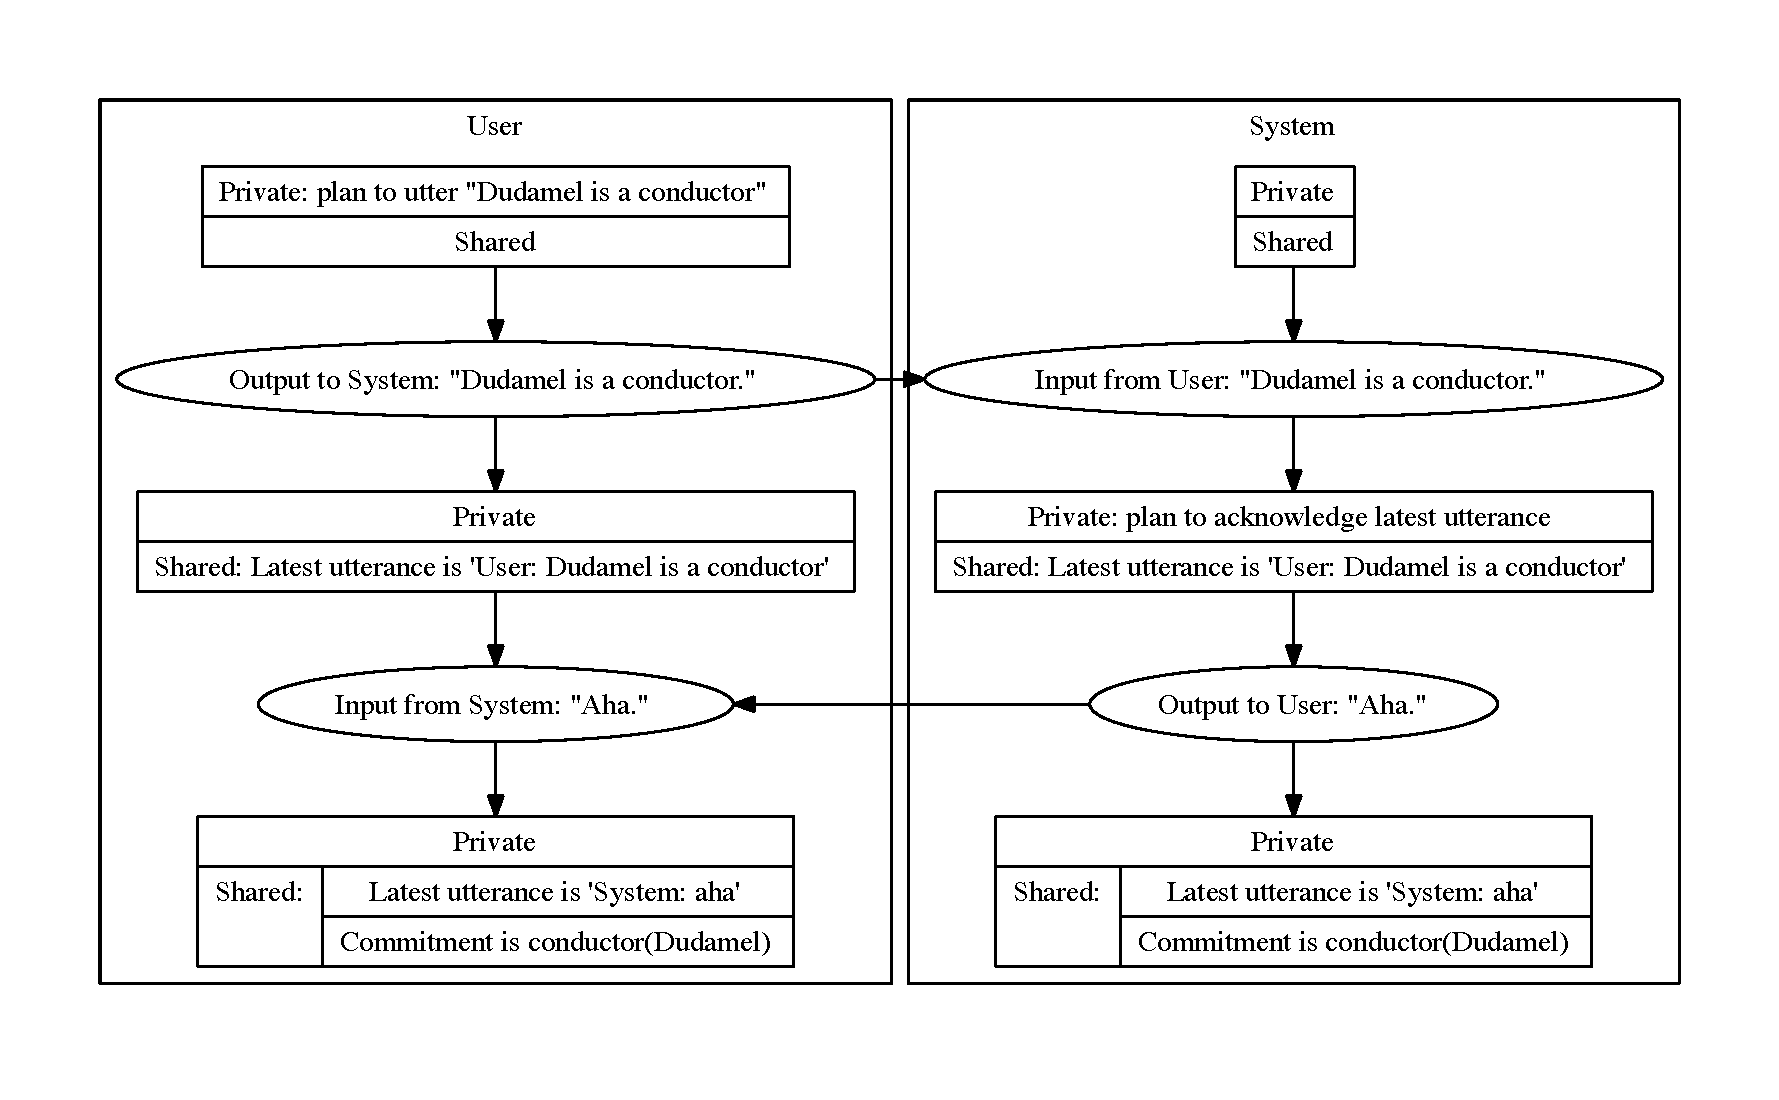
\includegraphics[width=\textheight]{simple-dm-diac}
\caption{Dialogue management:``Dudamel is a conductor''}
\label{fig:simple-dm-diac}
\end{sidewaysfigure}

%\clearpage

This assumes ideal
communication.  There is lots that could go wrong which could have the
consequence that the two agents become misaligned and an important
part of this framework is to provide a basis for the description of
miscommunication as well as communication.  (See
\cite{Ginzburg2012} for more discussion of this.)


We treat the dialogue information states represented by the square
boxes as records as in \nexteg{}.  


\begin{ex} 
\record{\field{private}{\record{\field{agenda}{\textit{AGENDA}}}} \\
        \field{shared}{\record{\field{latest-utterance}{\textit{L-UTT}} \\
                               \field{commitments}{\textit{COMM}}}}} 
\end{ex} 
  

What kinds of objects should \textit{AGENDA}, \textit{L-UTT} and
\textit{COMM} be?  % They will be defined with respect to the agent who
% owns the information state which, for convenience, we will refer to as
% \textit{SELF}.  We will see as we proceed with the discussion below
% that \textit{SELF} is related to the notion of \textit{de se} type act discussed in Section~\ref{sec:typeacts}.

We will say that \textit{AGENDA} is a list of sign \ignore{dialogue move} types,
that is,  the types of sign \ignore{dialogue moves} that the agent \ignore{\textit{SELF}} plans to
realize by means of a creation type act.  Recall from
Chapter~\ref{ch:percint} that this does not necessarily mean that
the agent \ignore{\textit{SELF}} is the main actor in the event
realizing the sign \ignore{move} type.
It can for example be a type of move to be carried out by an
interlocutor which the agent \ignore{\textit{SELF}} should wait for.  This will give us a
mechanism for handling basic turn-taking in dialogue.  (See
\citealp{SacksSchegloffJefferson1974} for the classic work on
turn-taking.) % We will define a dependent type \textit{Move} such that for any agent
% $A$, \textit{Move}($A$) is the type of dialogue moves in which $A$ is involved.
For now we will say that there are two ways in which an agent can be
involved in a dialogue act:  as speaker (or performer) or as hearer
(part of the audience to whom the dialogue act is
addressed).\footnote{A third way of being involved in a dialogue act
  which we will not take account of here is as an overhearer.}  % Performing a dialogue move is a \textit{de se} type act of creation as
% discussed in Chapter~\ref{sec:typeacts}.  Being the hearer or audience
% of a move type involves a \textit{de se} type act of judgement as
% discussed there.
% \textit{AGENDA}  should thus be a list of move types depending on
% \textit{SELF} (that
% is, subtypes of \textit{Move}(\textit{SELF})).  We introduce a
% dependent type,
% \textit{MoveType}, such that for any $a$:\textit{Ind},
% $T$:\textit{MoveType}($a$) iff $T\sqsubseteq\textit{Move}(a)$.
% \textit{AGENDA} is thus a list of move types and will
% have type [\textit{MoveType}(\textit{SELF})].   For any type $T$, $[T]$ is the type of
% lists all of whose members are of type $T$ (see
% Appendix~\ref{app:listtypes}).  We will come back to the details of
% \textit{Move} below.
% \todo{Move vs Sign?}

\textit{L-UTT} should tell us what the latest utterance in the
dialogue was.  This will be the witness of a sign type.  % move (or moves\footnote{See
%   \cite{Larsson2002} for a proposal where dialogue contributions
%   involve several moves. For now we will make the simplifying
%   assumption that utterances are associated with a single move.}) has just been carried out.
% But we will need more information than this.  We will need information about
% what (the agent \textit{SELF} thinks) was actually said.  For this we will use a
% chart, i.e. a set of edges between vertices representing hypotheses
% about parts of the utterance, that is, sign types associated with
% parts of the utterance.  The move should be predictable from the chart
% by a process of move-interpretation for which we will use the
% predicate `m-interp'.  Thus \textit{L-UTT} should itself be of
% the type \nexteg{}.

% \begin{ex} 
% \record{\tfield{move}{\textit{Move}(\textit{SELF})} \\
%         \tfield{chart}{\textit{Chart}} \\
%         \tfield{e}{m-interp(chart,move)}} 
% \end{ex} 
  

% The type \textit{Chart}
% we will say more about in Chapter~\ref{ch:gram}.

The commitments field has normally been considered as a set of
facts or propositions \citep{Ginzburg2012,Larsson2002}.  Here we will
treat them as a single record type, i.e. a witness of the type
\textit{RecType}.  Using a single type will make it more
straightforward to deal with issues like consistency and anaphora as
we will see in later chapters.

Thus information states can belong to the type \nexteg{}, our current
version of the type \textit{InfoState}.

\begin{ex} 
  \record{
    \tfield{private}{
      \record{
        \tfield{agenda}{$\mathrm{list}(\textit{RecType})$}}} \\
    \tfield{shared}{
      \record{
        \tfield{latest-utterance}{\textit{Sign}$^*$}\\
        \tfield{commitments}{\textit{RecType}}}}} 
\label{ex:InfoStatePrelim}
\end{ex}
Here \textit{Sign}$^*$ is the type of strings of signs of length 0 or
more using the string type notation introduced on
p.~\pageref{pg:stringtype-notation}.  At the beginning of a dialogue
there will be no latest utterance and we will represent this by having
the empty string of signs in `latest-utterance'-field.  By using
\textit{Sign}$^*$ we allow for the possibility that the previous
utterance can be represented by a string of several signs although in
the examples we will discuss here we will only have strings of length 1.

% (Here, by convention the labels `chart' and `move' in
% \smallrecord{\smalltfield{e}{m-interp(chart,move)}} refer to the path down to the minimal record in
% which the e-field occurs, that is `shared.latest-utterance.chart' and
% `shared.latest-utterance.move' respectively.)

% \preveg{} is, however, not quite general enough.  It requires that
% there always will be a latest utterance.  At the beginning of a
% dialogue this will not be the case and we need a way of representing
% that there is no previous utterance.  We will use a type whose only
% witness is the empty record for this.  Records, it will be recalled,
% are sets of ordered pairs (see
% Appendix~\ref{app:rectypes}).  This will include the empty set,
% $\emptyset$ which could also be notated as `[\ ]' if we are thinking
% of the empty set as the empty record.  However, this latter notation
% is confusing since it could also be used to represent the empty record
% type, that is the type that does not place any constraints on which
% records it has as witnesses, that is, the type of all records which we
% represent as \textit{Rec} in order to avoid confusion.  The type of
% the empty record could be constructed as the singleton type
% \textit{Rec}$_\emptyset$ (or if you are using the bracket notation for
% the empty record, \textit{Rec}$_{[\ ]}$).  In order to avoid
% notational confusion we will use \textit{ERec} to represent the type
% whose only witness is the empty record, that is, the empty set.  Thus
% \nexteg{} will hold.
% \begin{ex} 
% $a$ : \textit{ERec} iff $a=\emptyset$ 
% \end{ex} 
At the beginning of a
dialogue there will not be any shared commitments either.  Therefore, it
will be natural to use \textit{Rec} for the
commitments at the beginning of a dialogue.  \textit{Rec} is the type
of all records.  If we think of records as modelling situations then a
commitment represented by
\textit{Rec} is a commitment to the existence of a situation but not
to a situation of any particular type.  Thus it corresponds to ``there
is a situation'' or ``the world is not empty''.  It plays a similar
role in our theory to the set of all possible worlds in a system based
on possible worlds.  It represents a state where no constraints have
been placed on the nature of the world.   % The 
% adjustment we need to make to (\ref{ex:InfoStatePrelim}) in order to include dialogue
% initial information states is to the shared.latest-utterance field as
% in \nexteg{}.
% The `commitments'-field does not need to be adjusted as
The type \textit{Rec} is one of the witnesses of \textit{RecType} (see
Appendix~\ref{app:rectypes}).  The type of an initial information
state based on \preveg{} is \nexteg{}, that is, our current version of
the type \textit{InitInfoState}.
\begin{ex}
 \record{
    \tfield{private}{
      \record{
        \mfield{agenda}{[ ]}{$\mathrm{list}(\textit{RecType})$}}} \\
    \tfield{shared}{
      \record{
        \mfield{latest-utterance}{$\varepsilon$}{\textit{Sign}$^*$}\\
        \mfield{commitments}{\textit{Rec}}{\textit{RecType}}}}}   
% \smallrecord{\smalltfield{private}{\smallrecord{\smalltfield{agenda}{[\textit{MoveType}(\textit{SELF})]}}} \\
%         \smalltfield{shared}{\smallrecord{\smalltfield{latest-utterance}{\smallrecord{\smalltfield{move}{\textit{Move}(\textit{SELF})} \\
%                                                                   \smalltfield{chart}{\textit{Chart}}
%                                                                 \\
%                                                                   \smalltfield{e}{m-interp(chart,move)}}$\vee$\textit{ERec}}\\
%                                \smalltfield{commitments}{\textit{RecType}}}}}
% \label{ex:gameboard}
\end{ex}
% \preveg{} uses a join type (Appendix~\ref{app:jointypes}).  For any two
% types $T_1$ and $T_2$ you can form the join (or disjunction) $T_1\vee
% T_2$.  $a:T_1\vee T_2$ just in case either $a:T_1$ or $a:T_2$.

% \label{pg:SELF}We will use notation including `\textit{SELF}' as in \preveg{} to
% represent types which are derived from dependent types by applying
% them to the argument represented by \textit{SELF}.  This notational
% convention will save us a good deal of complication in presentation
% and it is always possible to recover the dependent type from which the
% type is derived by creating a function which maps an individual to the
% appropriate type.  Thus in the case of \preveg{} the dependent type
% would be \nexteg{}.
% \begin{ex}
% $\lambda a$:\textit{Ind} . \smallrecord{\smalltfield{private}{\smallrecord{\smalltfield{agenda}{[\textit{MoveType}($a$)]}}} \\
%         \smalltfield{shared}{\smallrecord{\smalltfield{latest-utterance}{\smallrecord{\smalltfield{move}{\textit{Move}($a$)} \\
%                                                                   \smalltfield{chart}{\textit{Chart}}
%                                                                 \\
%                                                                   \smalltfield{e}{m-interp(chart,move)}}$\vee$\textit{ERec}}\\
%                                \smalltfield{commitments}{\textit{RecType}}}}}
% \end{ex} 
% [???? This needs revising in order to include moves by agents other
% than \textit{SELF}!]

Some signs (but not all) will be associated with an \textit{illocutionary
force}, a term which originally comes from \cite{Austin1962}.  The four illocutionary forces we will consider here are:
assertion, query, command and acknowledgement.  Signs which have an
illocutionary force can be thought of as \textit{dialogue moves} or in
Austin's original terminology \textit{illocutionary acts}.
Those signs which are not associated with an illocutionary force are
normally constituents of something which does have illocutionary
force.  Thus, for example, if somebody says \textit{The dog barked}
the whole utterance can be thought of as an assertion.  However, the
utterance of \textit{the dog} which is part of this utterance does not
have illocutionary force.  This is not to say that some other
utterance of \textit{the dog} could not have illocutionary force.  For
example, in response to the question \textit{What made all the mess?},
an utterance of \textit{the dog} might be regarded as an assertion
that the dog made all the mess.

% Dialogue moves are a type of
% event in which an actor (normally speaker) is related to an intended
% audience, an illocutionary force (such as `assert') and a content
% (that is, for our present purposes, a record type such as \smallrecord{\smalltfield{e}{conductor(Dudamel)}}).

% , e.g. assert(User, System,
% conductor(Dudamel)).  We shall need to refine our view of what the
% third argument is.  But for now let us note that assert($a$,$b$,$c$)
% is a \textit{type}.  An object of this type will be an event or
% situation in which $a$ asserts $c$ with $b$ as the intended
% audience. ($b$ may or may not be able hear or comprehend $a$'s
% utterance.)  For technical reasons we will not use this type but one
% where the illocutionary force \textit{assert} is an argument:
% move(User, System, assert, conductor(Dudamel)).  We will need to access the various
% components of move types so that we can partially specify them.
% Therefore we will use the record type

% We will take dialogue moves to be a pairing of speech acts and content.
% The type of speech acts (\textit{SpeechAct}) will be taken to be a
% subtype of the type of speech events (\textit{SEvent}) as defined in
% (\ref{ex:SEventLocSpAu}) on p.~\pageref{ex:SEventLocSpAu}.  In
% particular this will mean that there is a field in a speech act for
% the speaker (labelled by `sp') and another for the audience (labelled
% by `au').  More
% specifically we will take the type \textit{Move}($a$) to be an abbreviation for
% \nexteg{}. 
% \begin{ex} 
% % \record{\tfield{actor}{\textit{Ind}} \\
% %         \tfield{audience}{\{\textit{Ind}\}} \\
% %         \tfield{orientation}{eq(\textit{SELF},actor)$\vee$member(\textit{SELF},audience)}
% %         \\
% %         \tfield{i-force}{\textit{IForce}} \\
% %         \tfield{content}{\textit{RecType}} \\
% %         \tfield{e}{move(actor, audience, i-force, content)}}
% \smallrecord{\smalltfield{e}{\textit{SpeechAct}}} $\wedge$ (
% \smallrecord{\smalltfield{e}{\smallrecord{\smallmfield{sp}{$a$}{\textit{Ind}}}}}
% $\vee$
% \smallrecord{\smalltfield{e}{\smallrecord{\smallmfield{au}{$a$}{\textit{Ind}}}}}
% )
% $\wedge$ \textit{MoveContent} 
% \label{ex:Move-a}
% \end{ex}
% The type in \preveg{} is a
% meet type (Appendix~\ref{app:meettypes}).\footnote{Strictly speaking, this type should be
%   written with parentheses since we are assuming a binary meet
%   operation:
%   (\smallrecord{\smalltfield{e}{\textit{SpeechAct}}} $\wedge$ ((
% \smallrecord{\smalltfield{e}{\smallrecord{\smallmfield{sp}{$a$}{\textit{Ind}}}}}
% $\vee$
% \smallrecord{\smalltfield{e}{\smallrecord{\smallmfield{au}{$a$}{\textit{Ind}}}}}
% )
% $\wedge$ \textit{MoveContent})) 
%   but we will often omit parentheses for clarity.} If $T_1$ and $T_2$ are
% types, then an object $a$ is of type  $T_1\wedge T_2$ just in case
% $a:T_1$ and $a:T_2$.  

% Note that \preveg{} requires $a$ to be either the speaker or the
% audience of the speech act and does not rule out the possibility that
% $a$ is both speaker and audience (i.e. $a$ is talking to herself).

% We
% will not attempt a complete inventory of speech act types here.
% Preliminarily, we could define \textit{SpeechAct} to be
% \begin{quote}
% \textit{Assertion}$\vee$\textit{Query}$\vee$\textit{Command}$\vee$\textit{Acknowledgement},
% \end{quote}
% that
% is, a join type (Appendix~\ref{app:jointypes}) of all the available
% speech act types.\footnote{Strictly speaking, this type should be
%   written with parentheses since we are assuming a binary join
%   operation:
%   (\textit{Assertion}$\vee$(\textit{Query}$\vee$(\textit{Command}$\vee$\textit{Acknowledgement})))
%   but we will often omit parentheses for clarity.}  Something will be of
% this type just in case it is of at least one of the types of the
% join.
% Each of the speech act types are subtypes of \textit{SEvent}
% and can be defined as in \nexteg{}.
We introduce four subtypes of \textit{Sign}:
\textit{Assertion}, \textit{Query}, \textit{Command} and
\textit{Acknowledgement}.  These are characterized in \nexteg{}. 
\begin{ex}
\begin{tabular}[t]{lcl}
\textit{Assertion} & -- & % \textit{SEvent} \d{$\wedge$} 
% \smallrecord{\smalltfield{e}{\textit{Phon}} \\
%              \smalltfield{c$_{\mathrm{illoc}}$}{assertion(e)}}
  \record{
  \tfield{s-event}{\textit{SEvent}}\\
  \tfield{cont}{\textit{RecType}}\\
  \tfield{illoc}{assert(s-event, cont)}
  }
  \\
\textit{Query} & -- & % \textit{SEvent} \d{$\wedge$} 
% \smallrecord{\smalltfield{e}{\textit{Phon}} \\
% \smalltfield{c$_{\mathrm{illoc}}$}{query(e)}}
  \record{
  \tfield{s-event}{\textit{SEvent}}\\
  \tfield{cont}{\textit{Question}}\\
  \tfield{illoc}{query(s-event, cont)}
  }
  \\
\textit{Command} & -- & % \textit{SEvent} \d{$\wedge$} 
% \smallrecord{\smalltfield{e}{\textit{Phon}} \\
% \smalltfield{c$_{\mathrm{illoc}}$}{command(e)}}
  \record{
  \tfield{s-event}{\textit{SEvent}}\\
  \tfield{cont}{\textit{RecType}}\\
  \tfield{illoc}{command(s-event, cont)}
  }
  \\
\textit{Acknowledgement} & -- & % \textit{SEvent} \d{$\wedge$} 
% \smallrecord{\smalltfield{e}{\textit{Phon}} \\
% \smalltfield{c$_{\mathrm{illoc}}$}{acknowledgement(e)}}
  \record{
  \tfield{s-event}{\textit{SEvent}}\\
  \tfield{cont}{\textit{RecType}}\\
  \tfield{illoc}{acknowledge(s-event, cont)}
  }
  

\end{tabular} 
\end{ex}
Note that the type of the content varies with the illocutionary
force.  We use the type \textit{Question} for queries and
\textit{RecType} for the others.  We will say more about
\textit{Question} in later chapters.  It is quite likely that the
content type for commands should be something other than
\textit{RecType}, for example, the type \textit{Ppty} (``property'')
that we will develop in later chapters, but we do not have more to say
about commands in this work.  In a more complete treatment of
illocutionary force the nature of the speech event could also be made
to vary with illocutionary force.  For example, we could require
question syntax for queries, although that would not take account of
the fact that declarative sentence syntax can also be used to ask
questions.  It is not our aim here to give a detailed analysis of such
phenomena but to provide a general framework in which they could be
analyzed.

We will also introduce types \textit{AssertionType},
\textit{QueryType}, \textit{CommandType} and
\textit{AcknowledgementType} which are characterized in a similar way
to \textit{SignType} as in \nexteg{}.
\begin{ex} 
\begin{subex} 
 
\item $T:\textit{AssertionType}$ iff $T\sqsubseteq \textit{Assertion}$ 
 
\item $T:\textit{QueryType}$ iff $T\sqsubseteq \textit{Query}$

  
\item $T:\textit{CommandType}$ iff $T\sqsubseteq \textit{Command}$

  
\item $T:\textit{AcknowledgementType}$ iff $T\sqsubseteq \textit{Acknowledgement}$ 
 
\end{subex} 
   
\end{ex} 
  

% Here the subscript `illoc' stands for ``illocutionary'' indicating
% that the condition provides information about the illocutionary force
% of the speech act. The symbol \d{$\wedge$} represents the merge operation defined in
% Appendix~\ref{app:merge}.  In \preveg{} the relevant merges will be
% the unions of the sets of fields represented by \textit{SEvent} and
% the type consisting of the `e' and `illoc' fields.  This is
% illustrated in \nexteg{} for \textit{Assertion}. \nexteg{a} (where
% \textit{SEvent} is spelled out) is
% identical with \nexteg{b}.
% \begin{ex} 
% \begin{subex} 
 
% \item \record{\tfield{e-loc}{\textit{Loc}} \\
%         \tfield{sp}{\textit{Ind}} \\
%         \tfield{au}{\textit{Ind}} \\
%         \tfield{e}{\textit{Phon}} \\
%         \tfield{c$_{\mathrm{loc}}$}{loc(e,e-loc)} \\
%         \tfield{c$_{\mathrm{sp}}$}{speaker(e,sp)} \\
%         \tfield{c$_{\mathrm{au}}$}{audience(e,au)}} \d{$\wedge$} 
% \smallrecord{\smalltfield{e}{\textit{Phon}} \\
%              \smalltfield{c$_{\mathrm{illoc}}$}{assertion(e)}}
 
% \item \record{\tfield{e-loc}{\textit{Loc}} \\
%         \tfield{sp}{\textit{Ind}} \\
%         \tfield{au}{\textit{Ind}} \\
%         \tfield{e}{\textit{Phon}} \\
%         \tfield{c$_{\mathrm{loc}}$}{loc(e,e-loc)} \\
%         \tfield{c$_{\mathrm{sp}}$}{speaker(e,sp)} \\
%         \tfield{c$_{\mathrm{au}}$}{audience(e,au)} \\
%         \tfield{c$_{\mathrm{illoc}}$}{assertion(e)}}

 
% \end{subex} 
   
% \end{ex} 
  

% Finally, the type \textit{MoveContent} in (\ref{ex:Move-a}) relates the type
% of the content of the move to the type of the move.  We define it
% preliminarily as the join type in \nexteg{}.
% \begin{ex} 
% \record{\tfield{e}{\textit{Assertion}} \\
%         \tfield{cont}{\textit{RecType}} \\
%         \tfield{c$_{\mathrm{cont}}$}{content(e,cont)}}$\vee$
% \record{\tfield{e}{\textit{Query}} \\
%         \tfield{cont}{\textit{Question}} \\
%         \tfield{c$_{\mathrm{cont}}$}{content(e,cont)}}$\vee$
% \record{\tfield{e}{\textit{Command}} \\
%         \tfield{cont}{\textit{RecType}} \\
%         \tfield{c$_{\mathrm{cont}}$}{content(e,cont)}}$\vee$
% \record{\tfield{e}{\textit{Acknowledgement}}} 
% \end{ex} 
% Note that this allows for acknowledgements such as \textit{ok} not to
% have any content (although it does not prevent them from having content).  We will return later to discussion of whether this
% is a reasonable claim for acknolwedgements, while noting that this would  be one way of
% dealing with ``phatic'' communication such as greetings like \textit{Hello}.

% We place a condition on `self' that it be the ``ego'', that is, that
% it involves a situation which is of the type ego(self).  The idea is
% that this is a type \textit{de se} by which we mean that a judgement
% that a situation $s$ is of the type ego($a$) requires that $a$ is the
% individual making the judgement.  We do not have a formal treatment of
% this.  We have relativized our judgements in Appendix~\ref{app:ttr} to
% systems of types involving assignments to the basic types but not to
% the agent making the judgement.  We will not develop this further here
% but merely note that the perception of oneself as the actor or the
% audience of a dialogue move is an essentially \textit{de se}
% phenomenon. For recent discussion of and a survey of the literature on
% \textit{de se} phenomena see \cite{Ninan2010,Hanks2012}.
  

% We will be able to read partial information about
% a dialogue move from certain aspects of a speech-event.  For example,
% an utterance of \textit{ok}
% may tell us that the dialogue move is of type \nexteg{}.

% \begin{ex} 
% % \record{\tfield{actor}{\textit{Ind}} \\
% %         \tfield{audience}{\{\textit{Ind}\}} \\
% %         \tfield{orientation}{member(\textit{SELF},audience)} \\
% %         \mfield{i-force}{acknowledge}{\textit{IForce}} \\
% %         \tfield{content}{\textit{RecType}} \\
% %         \tfield{e}{move(actor, audience, i-force, content)}} 
% \record{\tfield{e}{\textit{Acknowledgement}} \\
%         \mfield{sp}{\textit{SELF}}{\textit{Ind}}}
% \end{ex} 
In order to find the content of an utterance of \textit{ok}, we look
to the content of the previous utterance.  Thus an utterance of
\textit{ok} following an utterance of \textit{Dudamel is a conductor}
will have the same content as the assertion,  namely \nexteg{}.
\begin{ex} 
\record{\tfield{e}{conductor(dudamel)}} 
\end{ex} 
Assigning \preveg{} as the content of \textit{Dudamel is a conductor}
involves the naive assumption that a proper name uniquely identifies a
particular individual.  We will develop a more sophisticated approach
to proper names in Chapters~\ref{ch:gram} and \ref{ch:propnames}.  
% An
% utterance of \textit{Dudamel is a conductor} may give us information
% about the type of speech act (\textit{Assertion}) and the content
% (\smallrecord{\smalltfield{e}{conductor(Dudamel)}}).  Note, however,
% that we only get such a fully specified content if we have a unique
% individual `Dudamel' whom we associate with utterances of the name
% \textit{Dudamel}.  If the resources we have available do not give us
% such an individual associated with \textit{Dudamel} then we only get
% the information that somebody named Dudamel is a conductor, that is,
% we may only get partial information about the content the speaker
% intended to communicate.  Consider the example \textit{Strauss is a
%   composer}.  There are at least two famous composers named Strauss
% (and also some more not so famous ones).  If our available resources
% give us two people associated with the name \textit{Strauss} we will
% not know which of them is being referred to.  Representing contents as record types will 
% enable us to handle this content underspecification. However, in order
% to do this we will need to abandon our current simplifying
% ``propositional logic'' assumption
% that sentences come as unanalyzed wholes associated with their
% contents.  This we will do in Chapter~\ref{ch:gram}.
% We will talk
% about the exact nature of the record type when we talk about semantics below.


% Not surprisingly, when we are dealing with an agenda as in (\ref{ex:gameboard}), a
% plan for future action, we have got ourselves into a situation
% where we need types rather than the objects.  The things that are on
% the agenda list are not actual events, but rather \textit{types} of
% events planned for the future.  Normally the types occurring on the
% agenda will be subtypes of \textit{Move}(\textit{SELF}), though we may wish to
% include types of events like looking something up in a database,
% i.e. non-speech events.

% For the most part types on the agenda will not be completely specified
% types.  That is they will not be types all of whose fields are
% manifest (restricted to particular objects of those types).
% Frequently it will be the case that we specify the content of the move
% but leave open the phonology, that is, the type will specify the
% content of what is to be said but not actually what is to be said or
% even perhaps which language it should.  We want, for example, to be able to
% say that a speaker is carrying out the same type of move independently of which
% language they are speaking.  Thus, if the user says to the system ``Dudamel is a conductor''
% or (in Swedish) ``Dudamel �r dirigent'' she will in both cases have carried out a
% move involving the assertion of the content \smallrecord{\smalltfield{e}{conductor(Dudamel)}}.  This abstraction will
% be important, for example, if we want to change language in the middle
% of a dialogue, as people sometimes do.\footnote{This phenomenon is
%   known as code-switching \citep{BullockToribio2009}.}  At the same time it is the
% normal case to continue a dialogue in the same language and thus we
% need to note which language was used in the previous utterance,
% i.e. keep track of what was actually said.  This information will be
% in the chart which is part of the latest move.  In the chart there
% will be
% more information about what was actually said which will be important when it comes to dealing
% with parts of the utterance for things like clarification and
% anaphora.  But this again requires us to abandon our current
% simplifying ``propositional logic'' assumption.
    

% We will assume that agents do not have complete
% information about the information state, that is, they reason in terms
% of \textit{types} of information state (that is, gameboards).
% The basic intuition behind our reasoning about information state
% updates can be expressed as in \nexteg{}.

% \begin{ex} 
% If $r_i$ : $T_i$, then $r_{i+1}$ : $T_{i+1}(r_i)$ 
% \end{ex} 
  

% That is, given that we believe that the current information state is
% of type $T_i$ (recall that we can come to this belief without having
% any belief about which specific information state is involved), then
% we can conclude that the next information state is of type $T_{i+1}$
% which can depend on the current information state.  According to this,
% we can have a hypothesis about the type of the next information state
% even though we may not know exactly what the current information state
% is.  Exactly which type the next information state belongs to depends,
% though, on the exact nature of the current information state.  Thus
% the dependency in our types provides us with an additional means for
% representing underspecification.

% This basic rule of inference corresponds to a function from records to
% record types, a function of type ($T_i$ $\rightarrow$ {\it
%   RecType\/}), that is, one kind of update function we were using in Chapter~\ref{ch:percint}.  Such a function is of
% the form \nexteg{}. 

% \begin{ex} 
% $\lambda r\!:\!T_i\ .\ T_{i+1}(r)$ 
% \end{ex} 
  

% Things are a litte more complicated than this, however, because this
% only represents the change from one information state to another,
% whereas in fact this change is triggered by a speech
% event which bears an appropriate relation to the current information
% state represented by $r$.  Thus we are actually interested in
% functions from the current information state to a function from events
% to the new information state, as in \nexteg{}.

% \begin{ex}
% $\lambda r\!:\!T_i\ .\ \lambda e\!:\!T_e(r)\ .\ T_{i+1}(r,e)$
% \label{eg:updateFun}
% \end{ex}

% This is the other kind of update function we were using in Chapter~\ref{ch:percint}.\footnote{This is
%   one of a number of ways of characterizing update in this kind of
%   framework.  One might for instance think of the type of the speech event as
%   being part of the current information state.  Also instead of using
%   an update function one can use a record type with a
%   `preconditions'-field and an `effect'-field.  Both
%   \cite{Ginzburg2012} and \cite{Larsson2002} have this kind of approach.}
Let us consider
the update function and update rule which the user could use in order to update her
information state after her own utterance of \textit{Dudamel is
  a conductor}.  This is modelled on the kind of integration rules
discussed in \cite{Larsson2002}.  The update function we wish to
characterize will be defined on information states which have some
assertion type as the first element on the agenda, that is the type in
\nexteg{}.
\begin{ex} 
\record{
    \tfield{private}{
      \record{
        \tfield{agenda}{
          \record{
            \tfield{fst}{\textit{AssertionType}}\\
            \tfield{rst}{$\mathrm{list}(\textit{RecType})$}}}}} \\
    \tfield{shared}{
      \record{
        \tfield{latest-utterance}{\textit{Sign}$^*$}\\
        \tfield{commitments}{\textit{RecType}}}}}  
\end{ex} 
Rather than writing out such types in our update functions we can
think of the objects in the domain of our update
function as meeting the requirement that they belong to two types as
in \nexteg{}.
\begin{ex} 
\begin{subex} 
 
\item \textit{InfoState} 
 
\item
  \record{
    \tfield{private}{
      \record{
        \tfield{agenda}{
          \record{
            \tfield{fst}{\textit{AssertionType}}}}}}}
 
\end{subex} 
   
\end{ex} 
A statement of the update function in terms of the abbreviation
\textit{InfoState} will not only save space but also be helpful as we
further develop our notion of what type \textit{InfoState} represents.
If we are just adding extra fields to the type \textit{InfoState},
that is we develop our theory monotonically just by adding more
detail, then we do not have to go back and revise the formulation of
the update functions based on earlier versions of the theory.

However, we still need to give a characterization of a single type
which will serve as the domain type of the update function.  One way
to do this is to use TTR's \textit{meet types} such as \nexteg{}.
\begin{ex} 
  (\textit{InfoState} $\wedge$
  \record{
    \tfield{private}{
      \record{
        \tfield{agenda}{
          \record{
            \tfield{fst}{\textit{AssertionType}}}}}}}) 
\end{ex} 
In general $a:(T_1\wedge T_2)$ just in case $a:T_1$ and $a:T_2$.

\begin{shaded}
We can introduce meet (also known as intersection or conjunctive
types) into a type system as in \nexteg{}, repeated in
Appendix~\ref{app:meettypes}.
\begin{ex} 
A system of complex types \textbf{TYPE}$_C$ = $\langle${\bf Type}, {\bf BType},
$\langle$\textbf{PType}, {\bf Pred}, \textbf{ArgIndices}, {\it
  Arity\/}$\rangle$, $\langle A,F\rangle$$\rangle$ \textit{has meet types} if
\begin{enumerate} 
 
\item for any $T_1,T_2 \in \mathbf{Type}$, $(T_1\wedge T_2) \in \mathbf{Type}$ 
 
\item for any $T_1,T_2 \in \mathbf{Type}$, $a:_{\mathbf{TYPE_C}}(T_1\wedge T_2)$ iff
  $a:_{\mathbf{TYPE_C}}T_1$ and $a:_{\mathbf{TYPE_C}}T_2$ 

\end{enumerate}
\label{ex:meettypes}
\end{ex} 
In our informal proof theoretic notation this can be represented as
\nexteg{}.
\begin{ex} 
  For $\Gamma$ a system of complex types
  \begin{subex} 
 
  \item
    \begin{prooftree}
      \hypo{\Gamma\vdash T_1\in\textbf{Type}}
      \hypo{\Gamma\vdash T_2\in\textbf{Type}}
      \infer2{\Gamma\vdash (T_1\wedge T_2)\in\textbf{Type}}
    \end{prooftree}
    
 
  \item
    \begin{prooftree}
      \hypo{\Gamma\vdash a:T_1}
      \hypo{\Gamma\vdash a:T_2}
      \infer2{\Gamma\vdash a:(T_1\wedge T_2)}
    \end{prooftree}

    
  \item
    \begin{prooftree}
      \hypo{\Gamma\vdash a:(T_1\wedge T_2)}
      \infer1{\Gamma\vdash a:T_1}
    \end{prooftree}

    
  \item
    \begin{prooftree}
      \hypo{\Gamma\vdash a:(T_1\wedge T_2)}
      \infer1{\Gamma\vdash a:T_2}
    \end{prooftree}
 
\end{subex} 
  
\end{ex} 
Just as we did for join types we can introduce a generalized version
of meet types as in \nexteg{}, repeated in Appendix~\ref{app:meettypes}.
\begin{ex} 
A system of complex types {\bf TYPE$_C$} = $\langle${\bf Type}, {\bf BType},
$\langle$\textbf{PType}, {\bf Pred}, \textbf{ArgIndices}, {\it
  Arity\/}$\rangle$, $\langle A,F\rangle$$\rangle$ \textit{has
  generalized meet
  types} if 

\begin{enumerate} 
 
\item for any non-empty finite set of types, $\mathbb{T}$, such that $\mathbb{T}
  \subseteq\mathbf{Type}$, $\bigwedge\mathbb{T} \in \mathbf{Type}$ 
 
\item for any finite $\mathbb{T} \subseteq\mathbf{Type}$, $a:_{\mathbf{TYPE_C}}\bigwedge\mathbb{T}$ iff
  $a:_{\mathbf{TYPE_C}}T$ for all $T\in\mathbb{T}$
 
\end{enumerate}
\label{ex:genmeettypes}
\end{ex} 
In our informal proof theoretic notation this can be represented as
\nexteg{}.
\begin{ex} 
  For $\Gamma$ a system of complex types
  \begin{subex} 
 
  \item
    \begin{prooftree}
      \hypo{\Gamma\vdash T_1,\ldots,T_n\in\textbf{Type}}
      \infer1{\Gamma\vdash\bigwedge\{T_1,\ldots,T_n\}\in\textbf{Type}}
    \end{prooftree}
    
 
  \item
    \begin{prooftree}
      \hypo{\Gamma\vdash a:T_1,\ldots,a:T_n}
      \infer1{\Gamma\vdash a:\bigwedge\{T_1,\ldots,T_n\}}
    \end{prooftree}

    
  \item
    \begin{prooftree}
      \hypo{\Gamma\vdash a:\bigwedge\{T_1,\ldots,T_n\}}
      \hypo{1\leq i\leq n}
      \infer2{\Gamma\vdash a:T_i}
    \end{prooftree}
    
 
\end{subex} 
  
\end{ex}
As with join types, we can, if we wish, use $T_1\wedge\ldots\wedge
T_n$ to represent $\bigwedge\{T_1,\ldots,T_n\}$.
  
\end{shaded}

If $T_1$ and $T_2$ are record types then there will always be a record
type (not a meet) 
$T_3$ which is necessarily equivalent to $T_1\wedge T_2$, that is any
record, $r$ of type $T_1\wedge T_2$ will be of type $T_3$ and
\textit{vice versa}.  We will call this the \textit{merge} of $T_1$
and $T_2$ which we will represent as $T_1$\d{$\wedge$}$T_2$ (with a dot
under `$\wedge$').  For example, \nexteg{a} will have the same set
of witnesses as \nexteg{b}.
\begin{ex} 
\begin{subex} 
 
\item  \record{\tfield{f}{$T_1$}}$\wedge$\record{\tfield{g}{$T_2$}}
 
\item \record{\tfield{f}{$T_1$}\\
        \tfield{g}{$T_2$}} 
 
\end{subex} 
   
\end{ex} 
When a label only occurs in one of the types being merged then the
field with that label is also a field of the merge of the two types.
Thus \nexteg{} holds.
\begin{ex} 
\record{\tfield{f}{$T_1$}}\d{$\wedge$}\record{\tfield{g}{$T_2$}} = \record{\tfield{f}{$T_1$}\\
        \tfield{g}{$T_2$}} 
\end{ex} 
When the same label, $\ell$, occurs in both types, then whatever
occurs in the $\ell$-field must be of the types required in those
fields by both the types.  Thus \nexteg{a} and \nexteg{b} will have
the same witnesses.
\begin{ex} 
\begin{subex} 
 
\item \record{\tfield{f}{$T_1$}}$\wedge$\record{\tfield{f}{$T_2$}} 
 
\item \record{\tfield{f}{$T_1\wedge T_2$}} 
 
\end{subex} 
   
\end{ex} 
In a case like this we will make the merge recursive down inside the
type, that is, we will make merge the types in the `f'-field in
\preveg{b}.  Thus \nexteg{} will hold.
\begin{ex} 
  \record{\tfield{f}{$T_1$}}\d{$\wedge$}\record{\tfield{f}{$T_2$}} =
  \record{\tfield{f}{$T_1$\d{$\wedge$}$T_2$}}
\end{ex} 
If one or the other of $T_1$ and $T_2$ is not a record type then
$T_1$\d{$\wedge$}$T_2$ will be $T_1\wedge T_2$.  If $T_1\sqsubseteq T_2$
then $T_1$\d{$\wedge$}$T_2$ is $T_1$ and if $T_2\sqsubseteq T_1$
then $T_1$\d{$\wedge$}$T_2$ is $T_2$.  

\begin{shaded}
We can define the merge operation on types in the following way
(repeated in Appendix~\ref{app:merge}).\label{pg:merge} The definition
is closely related to the unification algorithms used in feature based
grammar (see \citealp{Shieber1986} for the classic reference).

We define a function $\mu$ which maps meets of record types to an
equivalent record type, record types to equivalent types where meets
in their values have been simplified by $\mu$ and any other types to
themselves:
\begin{enumerate}
  \item if for some $T_1,T_2$, $T=(T_1\wedge T_2)$ and $T_1\sqsubseteq T_2$
  then $\mu(T)=T_1$ 
 
\item if for some $T_1,T_2$, $T=(T_1\wedge T_2)$ and $T_2\sqsubseteq T_1$
  then $\mu(T)=T_2$
  
\item otherwise:
\begin{enumerate} 
 
\item if for some $T_1$, $T_2$, $T=(T_1\wedge T_2)$ then
  $\mu(T)=\mu'(\mu(T_1)\wedge\mu(T_2))$. 
 
\item if $T$ is a record type then $\mu(T)$ is $T'$ such that for any
  $\ell$,$v$, $\langle\ell,\mu(v)\rangle\in T'$ iff
  $\langle\ell,v\rangle\in T$.

\item otherwise $\mu(T)=T$.
 
\end{enumerate}
\end{enumerate}

$\mu'(T_1\wedge T_2)$ is defined by:
\begin{enumerate} 
 
\item if $T_1$ and $T_2$ are record types, then $\mu'(T_1\wedge
  T_2)=T_3$ such that
\begin{enumerate} 
 
\item for any $\ell,v_1,v_2$, if $\langle\ell,v_1\rangle\in T_1$ and
  $\langle\ell,v_2\rangle\in T_2$, then 

\begin{enumerate} 
 
\item if $v_1$ and $v_2$ are
\begin{quote}
  $\langle\lambda u_1\!\!:\!\!T'_1\ldots\lambda
  u_i\!\!:\!\!T'_i\ .\ \phi,\langle\pi_1\ldots\pi_i\rangle\rangle$
  \end{quote}
  and
  \begin{quote}
    $\langle\lambda u'_1\!\!:\!\!T''_1\ldots\lambda
  u'_k\!\!:\!\!T''_k\ .\ \psi,\langle\pi'_1\ldots\pi'_k\rangle\rangle$
\end{quote}
respectively, then
\begin{quote}
$\langle\lambda u_1\!\!:\!\!T'_1\ldots\lambda
  u_i\!\!:\!\!T'_i,\lambda u'_1\!\!:\!\!T''_1\ldots\lambda
  u'_k\!\!:\!\!T''_k\ .\ \mu(\phi\wedge\psi), \langle\pi_1\ldots\pi_i,\pi'_1\ldots\pi'_k\rangle\rangle\in T_3$
\end{quote}

\item if $v_1$ is
  \begin{quote}
$\langle\lambda u_1\!\!:\!\!T'_1\ldots\lambda
u_i\!\!:\!\!T'_i\ .\ \phi,\langle\pi_1\ldots\pi_i\rangle\rangle$
\end{quote}
and $v_2$ is a
  type (i.e. not of the form $\langle f,\Pi\rangle$ for some function
  $f$ and sequence of paths $\Pi$), then
  \begin{quote}
    $\langle\lambda u_1\!\!:\!\!T'_1\ldots\lambda
  u_i\!\!:\!\!T'_i\ .\ \mu(\phi\wedge
  v_2),\langle\pi_1\ldots\pi_i\rangle\rangle\in T_3$
\end{quote}

\item if $v_2$ is
  \begin{quote}
    $\langle\lambda u'_1\!\!:\!\!T''_1\ldots\lambda
  u'_k\!\!:\!\!T''_k\ .\
  \psi),\langle\pi'_1\ldots\pi'_k\rangle\rangle$
\end{quote}
and $v_1$
is a type, then
\begin{quote}
  $\langle\lambda u'_1\!\!:\!\!T''_1\ldots\lambda
  u'_k\!\!:\!\!T''_k\ .\ \mu(v_1\wedge\psi)),\langle\pi'_1\ldots\pi'_k\rangle\rangle\in
  T_3$
  \end{quote}

\item otherwise $\langle\ell,\mu(v_1\wedge
  v_2)\rangle\in T_3$ 
 
\end{enumerate} 
  


 
\item for any $\ell,v_1$, if $\langle\ell,v_1\rangle\in T_1$ and there
  is no $v_2$ such that $\langle\ell,v_2\rangle\in T_2$, then
  $\langle\ell,v_1\rangle\in T_3$

\item for any $\ell,v_2$, if $\langle\ell,v_2\rangle\in T_2$ and there
  is no $v_1$ such that $\langle\ell,v_1\rangle\in T_1$, then
  $\langle\ell,v_2\rangle\in T_3$
 
\end{enumerate} 

% \item if $T_1$ and $T_2$ are record types and $T_2\sqsubseteq T_1$, then
%   $\mu'(T_1\wedge T_2)=T_2$

% \item if $T_1$ and $T_2$ are record types and $T_1\sqsubseteq T_2$, then
%   $\mu'(T_1\wedge T_2)=T_1$

\item if $T_1$ is $\mathrm{list}(T_1')$ ($\mathrm{set}(T_1')$, $\mathrm{plurality}(T_1')$) and
  $T_2$ is $\mathrm{list}(T_2')$ ($\mathrm{set}(T_2')$, $\mathrm{plurality}( T_2')$), then
  $\mu'(T_1\wedge T_2)=\mathrm{list}(\mu(T_1'\wedge T_2'))$ ($\mathrm{set}(\mu(T_1'\wedge
  T_2'))$, $\mathrm{plurality}(\mu(T_1'\wedge T_2'))$)
   
 
\item \label{item:mergeotherwise} otherwise $\mu'(T_1\wedge T_2)=T_1\wedge T_2$ 
 
\end{enumerate} 

$(T_1$ \d{$\wedge$} $T_2)$ is used to represent $\mu(T_1\wedge T_2)$.
We call  $(T_1$ \d{$\wedge$} $T_2)$ the \textit{merge} of $T_1$ and
$T_2$.

It is important for this characterization of merge to work properly
that paths in record types extend into meet types within the record
type.  Consider the merge expressed in \nexteg{a} where we assume that
\textit{Sit} is a basic type, for example the type of situations.
According to the above definition \nexteg{a} will be identical with
\nexteg{b}.
\begin{ex} 
\begin{subex} 
 
\item \record{
    \tfield{e}{\record{
        \tfield{x}{\textit{Ind}}\\
        \tfield{y}{\textit{Ind}}\\
        \tfield{e}{hug(x,y)}}} \\
    \tfield{c$_1$}{boy(e.x)}\\
    \tfield{c$_2$}{dog(e.y)} 
  } \d{$\wedge$} \record{\tfield{e}{\textit{Sit}}} 
 
\item \record{
    \tfield{e}{\record{
        \tfield{x}{\textit{Ind}}\\
        \tfield{y}{\textit{Ind}}\\
        \tfield{e}{hug(x,y)}} $\wedge$ \textit{Sit}} \\
    \tfield{c$_1$}{boy(e.x)}\\
    \tfield{c$_2$}{dog(e.y)} 
  } 
 
\end{subex} 
\label{ex:paths-into-meets}   
\end{ex} 
If the paths of record types do not extend into meet types then the
paths of \preveg{b} would be \nexteg{} and \preveg{} would not be a
well-formed record type since the `c$_1$' and `c$_2$'-fields would
reference non-existant paths.
\begin{ex} 
\{e, c$_1$, c$_2$\} 
\end{ex} 
However, clearly any record which is of the type (\ref{ex:paths-into-meets}b)  must in addition
have the paths `e.x' and `e.y' because of the requirement expressed by
the meet type.  Thus it is appropriate and intuitive that these should
count as paths in the record type thus making
(\ref{ex:paths-into-meets}b) well-formed.  


\end{shaded}

In our update action rules we will make use of an operation called
\textit{asymmetric merge}.\label{pg:asymmerge}  The asymmetric merge of types $T_1$ and
$T_2$, $T_1$\fbox{\d{$\wedge$}}$T_2$ is like their merge except that
if either $T_1$ or $T_2$ is not a record type then
$T_1$\fbox{\d{$\wedge$}}$T_2$ is $T_2$.  Also asymmetric merge does
not check for subtyping in the way that ordinary merge does.  Thus
when asymmetrically merging non-record types, $T_1$ and $T_2$,
$T_1$\fbox{\d{$\wedge$}}$T_2$ will always be $T_2$ regardless of
whether the subtype relation holds between the two types.

\begin{shaded}
We can define asymmetric merge in the following way (repeated in
Appendix~\ref{app:merge}).  The definition is closely related to the
priority unification algorithms used in feature based grammar
\citep{Shieber1986}.

The \textit{asymmetric merge} of $T_1$ and
$T_2$ is defined by a function, $\mu_{\mathrm{asym}}$, exactly
like $\mu$ except that the first two clauses of the definition of
$\mu$ are missing and $\mu'$ is replaced by another function
$\mu_{\mathrm{asym}}'$.  Thus the definition of $\mu_{\mathrm{asym}}$
is:
\begin{enumerate} 
 
\item if for some $T_1$, $T_2$, $T=(T_1\wedge T_2)$ then
  $\mu_{\mathrm{asym}}(T)=\mu_{\mathrm{asym}}'(\mu_{\mathrm{asym}}(T_1)\wedge\mu_{\mathrm{asym}}(T_2))$. 
 
\item if $T$ is a record type then $\mu_{\mathrm{asym}}(T)$ is $T'$ such that for any
  $\ell$,$v$, $\langle\ell,\mu_{\mathrm{asym}}(v)\rangle\in T'$ iff
  $\langle\ell,v\rangle\in T$.

\item otherwise $\mu_{\mathrm{asym}}(T)=T$.
 
\end{enumerate}

The definition of $\mu_{\mathrm{asym}}'$ is exactly like $\mu'$,
replacing $\mu$ and $\mu'$ with $\mu_{\mathrm{asym}}$ and $\mu_{\mathrm{asym}}'$ respectively, except that
the
clause~\ref{item:mergeotherwise} of the definition of $\mu'$ is replaced by 
\begin{enumerate} 
 
\item[\ref{item:mergeotherwise}$'$.] otherwise $\mu_{\mathrm{asym}}'(T_1\wedge T_2)=T_2$ 
 
\end{enumerate} 
  
We use $T_1$ \fbox{\d{$\wedge$}} $T_2$  to represent the asymmetric
merge of $T_1$ and $T_2$.  

Asymmetric merge may result in an ill-formed record type if we take
the asymmetric merge of a record type, $T_1$, and a non-record type,
$T_2$, since $T_1$ may be embedded in a larger type with fields
dependent on paths into $T_1$ which will not be present in the result
where $T_2$ has been substituted for $T_1$ thus removing the relevant
paths.  Consider the asymmetric merge \nexteg{a} which is \nexteg{b},
where, as above, \textit{Sit} is a basic type.
\begin{ex} 
\begin{subex} 
 
\item \record{
    \tfield{e}{\record{
        \tfield{x}{\textit{Ind}}\\
        \tfield{y}{\textit{Ind}}\\
        \tfield{e}{hug(x,y)}}} \\
    \tfield{c$_1$}{boy(e.x)}\\
    \tfield{c$_2$}{dog(e.y)} 
  } \fbox{\d{$\wedge$}} \record{\tfield{e}{\textit{Sit}}} 
 
\item \record{
    \tfield{e}{\textit{Sit}} \\
    \tfield{c$_1$}{boy(e.x)}\\
    \tfield{c$_2$}{dog(e.y)} 
  } 
 
\end{subex} 

\end{ex} 
\preveg{b} is clearly not a well-formed type since the fields labelled
by `c$_1$' and `c$_2$' address non-existent paths.

\end{shaded}

Armed with this technology we can define an update function,
f$_{\textsc{PlanAckAss}}$,  and action
rule which plan an acknowledgement to an assertion as in \nexteg{}.
\begin{ex} 
\begin{subex} 
 
\item f$_{\textsc{PlanAckAss}}$

  $\lambda r$:\textit{InfoState} . \\
  \hspace*{2em}$\lambda u$:\textit{Assertion} . \\
  \hspace*{4em}
  \smallrecord{
    \smalltfield{private}{\smallrecord{
        \smalltfield{agenda}{\smallrecord{
            \smalltfield{fst}{\smallrecord{
                \smalltfield{s-event}{\textit{SEvent} \d{$\wedge$} \smallrecord{
                    \smallmfield{sp}{$u$.s-event.au}{\textit{Ind}}\\
                    \smallmfield{au}{$u$.s-event.sp}{\textit{Ind}}}}\\
                \smallmfield{cont}{$u$.cont}{\textit{Cont}}\\
                \smalltfield{illoc}{acknowledge(s-event, cont)}}}\\
            \smallmfield{rst}{$r$.private.agenda}{$\mathrm{list}(\textit{RecType})$}}}}}\\
    \smalltfield{shared}{\smallrecord{
        \smallmfield{latest-utterance}{$u$}{\textit{Assertion}}}}}
        
 
\item \textsc{PlanAckAss}

  \begin{prooftree}
    \hypo{s_{i,A}:_A T_{\mathrm{curr}}}
    \hypo{T_{\mathrm{curr}}\sqsubseteq\mathrm{domtype}(\text{f}_{\textsc{PlanAckAss}})}
    \hypo{u^*:_A T_{\mathrm{utt}}}
    \hypo{T_{\mathrm{utt}}\sqsubseteq\textit{Assertion}}
    \infer[enth]4{s_{i+1,A}:_A
      T_{\mathrm{curr}}\text{\fbox{\d{$\wedge$}}}(\text{f}_{\textsc{PlanAccAss}}(s_{i,A})(u^*)\text{\d{$\wedge$}}\text{\smallrecord{\smalltfield{shared}{\smallrecord{
              \smalltfield{latest-utterance}{$T_{\mathrm{utt}}$}}}}})}
  \end{prooftree}
  
 
\end{subex} 
   
\end{ex} 
  





% \begin{ex} \mbox{}

% \hspace*{-3em}\begin{minipage}{\textwidth}$\lambda
% r$:\record{\tfield{private}{\record{\tfield{agenda}{$_{\mathit{ne}}$[\textit{MoveType}(\textit{SELF})]}}}}
% \\
% \hspace*{2em}$\lambda
% u$:\record{\tfield{move}{fst($r$.private.agenda)
% \d{$\wedge$}
% \smallrecord{\smalltfield{e}{\smallrecord{\smallmfield{sp}{\textit{SELF}}{\textit{Ind}}
%       \\
%                                           \smalltfield{au}{\textit{Ind}}}}}
% \d{$\wedge$}
% \smallrecord{\smalltfield{e}{\textit{Assertion}}}} \\
%                                 \tfield{chart}{\textit{Chart}} \\
%                                 \tfield{e}{m-interp(chart,move)}}\hspace*{.5em}. \\
% \hspace*{4em}\smallrecord{\smalltfield{private}{\smallrecord{\smallmfield{agenda}{\begin{tabular}{l}
% \smallrecord{\smalltfield{e}{\textit{Acknowledgement}\d{$\wedge$}\smallrecord{\smallmfield{sp}{$u$.move.e.au}{\textit{Ind}}
%       \\
%                                                                            \smallmfield{au}{\textit{SELF}}{\textit{Ind}}}}
%                                                                        \\
%              \smallmfield{cont}{$u$.move.cont}{\textit{RecType}} \\
%              \smalltfield{c$_{\mathrm{cont}}$}{content(e,cont)}}  \\
% \hspace*{10em}$\mid$ rst($r$.private.agenda) \end{tabular}}{[\textit{MoveType}(\textit{SELF})]}}}
%   \\
%                       \smalltfield{shared}{\smallrecord{\smalltfield{latest-utterance}{\smallrecord{\smallmfield{move}{$u$.move}{\textit{Move}(\textit{SELF})} \\
%                                                                                 \smallmfield{chart}{$u$.chart}{\textit{Chart}}
%                                                                               \\
% \smallmfield{e}{$u$.e}{m-interp(chart,move)}}}}}}
% \end{minipage}
% \label{eg:updateFunIntegOwn}

% \end{ex}



\preveg{a} maps information states (records), $r$, to a function that maps events to a type of information
state. The second
argument to the function (represented by $u$) requires a 
speech event  which is an assertion.  The type that results from applying the function to
its arguments represents the effect of the update.
This type requires the agenda to be result of pushing the type of an
acknowledgement of the content of $u$ onto the agenda and recording
$u$ as the latest utterance.  It also requires that the speaker of the
acknowledgement is the addressee of $u$ and that the addressee of the
acknolwedgement be the speaker of $u$.  The content of the acknowledgement is the same as
the content of the assertion.  That is, what is being acknowledged is
the content of the assertion.

\preveg{b} we give the action rule \textsc{PlanAckAss} which
characterizes the conditions under which  an agent
$A$ can be licensed to plan to acknowledge an assertion.  As before we
use $s_{i,A}$ for $A$'s current information state and $s_{i+1,A}$ for
$A$'s updated information state.  $T_{\mathrm{curr}}$ is used for the
type $A$ assigns to her current information state.  $u^*$ is used for
the current utterance and $T_{\mathrm{utt}}$ for the type that $A$
assigns to the current utterance.  The rule says that if
$T_{\mathrm{curr}}$ is a subtype of the domain type of the update
function \preveg{a} and $T_{\mathrm{utt}}$ is a subtype of
\textit{Assertion} then $A$ is licensed to judge that her updated
information state is of the type $T_{\mathrm{curr}}$ asymmetrically
merged with the result of applying the update function to the current
information state and the current utterance and merged with the
information that the latest utterance is of type $T_{\mathrm{utt}}$.



% We will now examine how such an update function could be used to
% reason about an update.  Let us suppose that the user considers the current information state
% to be of type:

% \begin{ex}
% \smallrecord{\smalltfield{private}{\smallrecord{\smallmfield{agenda}{[
%                    \smallrecord{\smalltfield{e}{\textit{Assertion}
%                      \d{$\wedge$} \smallrecord{\smallmfield{sp}{\textit{SELF}}{\textit{Ind}}}}                               \\
%                                 \smallmfield{cont}{\smallrecord{\smalltfield{e}{conductor(dudamel)}}}{\textit{RecType}}
%                                 \\
%                                 \smalltfield{c$_{\mathrm{cont}}$}{content(e,cont)}}
% ]
% }{[\textit{RecType}]}}} \\
%         \smalltfield{shared}{\smallrecord{\smalltfield{latest-utterance}{\textit{ERec}}\\
%                                \smallmfield{commitments}{\textit{Rec}}{\textit{RecType}}}}}
% \label{eg:initialInfoDiac}
% \end{ex}

% This represents that the user intends to assert that Dudamel is a conductor
% represented by the record type
% \smallrecord{\smalltfield{e}{conductor(Dudamel)}}.  
% The user also believes that there was no previous utterance and no commitments,
% i.e. that the planned utterance will be dialogue initial.  
% % Given the
% % assumption that information states may not contain any additional fields, there is no question about what
% % the current information state is.  It must be:

% % \record{\field{private}{\record{\field{agenda}{$\left[\mbox{\smallrecord{\smallmfield{actor}{User}{\textit{Ind}} \\
% %                                                               \smallmfield{audience}{System}{\{\textit{Ind}\}} \\
% %                                                               \smallmfield{i-force}{assert}{\textit{IForce}} \\
% %                                                               \smallmfield{content}{\smallrecord{\smalltfield{c}{conductor(Dudamel)}}}{\textit{RecType}} \\
% %                                                               \smalltfield{c}{move(actor, audience, i-force, content)}}}\right]$}}} \\
% %         \field{shared}{\record{\field{latest-utterance}{\record{\field{moves}{$\emptyset$} \\
% %                                                                 \field{chart}{$\emptyset$}}}\\
% %                                \field{commitments}{[]}}}}

% Suppose now that the user utters \textit{Dudamel is a conductor} and
% judges this utterance event $u_1$ to be an event of type \nexteg{}.
% \begin{ex} 
%  \record{\tfield{move}{\smallrecord{\smalltfield{e}{\textit{Assertion}\d{$\wedge$} \smallrecord{\smallmfield{sp}{\textit{SELF}}{\textit{Ind}}}} 
%                                 \\
%                                 \smallmfield{cont}{\smallrecord{\smalltfield{e}{conductor(Dudamel)}}}{\textit{RecType}}
%                                 \\
%                                 \smalltfield{c$_{\mathrm{cont}}$}{content(e,cont)}}} \\
%           \tfield{chart}{\textit{Chart}} \\
%           \tfield{e}{m-interp(chart,move)}}
% \end{ex} 
  



% % \record{\field{moves}{\{$m$\}} \\
% %         \field{m}{$m$} \\
% %         \field{chart}{$K$}}

% % where $m$:\smallrecord{\smallmfield{actor}{User}{\textit{Ind}} \\
% %                        \smallmfield{audience}{System}{\{\textit{Ind}\}} \\
% %                        \smallmfield{i-force}{assert}{\textit{IForce}} \\
% %                        \smallmfield{content}{\smallrecord{\smalltfield{c}{conductor(Dudamel)}}}{\textit{RecType}} \\
% %                        \smalltfield{c}{move(actor, audience, i-force,
% %                          content)}}
% The user will have more information about the nature of the chart
% (that is, about what was actually said and how it might be analyzed) than
% we have represented but we will leave this underspecified for now.

% Clearly in the user's judgement the utterance $u_1$ fulfils the requirements
% placed on it by (\ref{eg:updateFunIntegOwn}) since the move
% interpretation associated with it is of the type which occurs at
% the head of the agenda.  Note that we are reasoning with this function without actually
% providing it with an argument since we only have a (hypothesized) type
% of the current information state, not the actual information state.
% The crucial judgement is that the type of the current information state is
% a subtype of the domain type of the function.  This is sufficient to
% allow us to come to a conclusion about the type of the new information
% state.  

% According to the update function the next information state
% must be of the type \nexteg{}.

% \begin{ex} 
% \smallrecord{\smalltfield{private}{\smallrecord{\smallmfield{agenda}{[\smallrecord{\smalltfield{e}{\textit{Acknowledgement}\d{$\wedge$}\smallrecord{\smallmfield{sp}{$u_1$.move.e.au}{\textit{Ind}}
%       \\
%                                                                            \smallmfield{au}{\textit{SELF}}{\textit{Ind}}}}
%                                                                        \\
%              \smallmfield{cont}{$u_1$.move.cont}{\textit{RecType}} \\
%              \smalltfield{c$_{\mathrm{cont}}$}{content(e,cont)}}]}{[\textit{RecType}]}}}
%   \\
%                       \smalltfield{shared}{\smallrecord{\smalltfield{latest-utterance}{\smallrecord{\smallmfield{move}{$u_1$.move}{\textit{Move}} \\
%                                                                                 \smallmfield{chart}{$u_1$.chart}{\textit{Chart}}
%                                                                               \\
% \smallmfield{e}{$u_1$.e}{m-interp(chart,move)}}}}}}\label{eg:typepr} 
% \end{ex} 
  

% % \record{\tfield{private}{\record{\mfield{agenda}{[]}{[\textit{Move}]}}}
% %   \\
% %                       \tfield{shared}{\record{\tfield{latest-utterance}{\record{\mfield{moves}{\{$m$\}}{\{\textit{Move}\}} \\
% %                                                                                 \mfield{chart}{$K$}{\textit{Chart}}}}}}}

% \ignore{
% Note that we could have come to this conclusion even without the
% simplifying assumption that information states cannot contain
% additional fields.  Even if the type had been less specified we could
% still have drawn the conclusion as long as the agenda field was
% specified, e.g. the user might have been unsure whether the dialogue
% was already started or not:

% \record{\tfield{private}{\record{\mfield{agenda}{[move(User, System, assert, conductor(Dudamel))]}{[\textit{Move}]}}} \\
%         \tfield{shared}{\record{\tfield{latest-utterance}{\record{\tfield{moves}{\{\textit{Move}\}} \\
%                                                                   \tfield{utterance}{\textit{Chart}}}}\\
%                                \tfield{commitments}{\textit{RecType}}}}}
% }
% But we know more about the new information state than what is
% expressed by the type which results from the update function.
% Everything we know about the current information state which remains unchanged by the function must be carried
% over from the current information state.  This is related to the frame
% problem introduced by \cite{McCarthyHayes1969}.\footnote{For a recent
%   overview of the frame problem see \cite{Shanahan2009}.}  We 
% handle this performing an \textit{asymmetric merge} (see
% Appendix~\ref{app:merge}) of the type we have for the current
% information state with the type
% resulting from the update function.  The asymmetric merge of two types
% $T_1$ and $T_2$ is represented by $T_1$\fbox{\d{$\wedge$}}$T_2$.  If
% one or both of $T_1$ and $T_2$ are 
% non-record types then $T_1$\fbox{\d{$\wedge$}}$T_2$ will be $T_2$. If
% they are both record types, then for any label $\ell$ which occurs in
% both $T_1$ and $T_2$, $T_1$\fbox{\d{$\wedge$}}$T_2$ will contain a
% field labelled $\ell$ with the type resulting from the asymmetric
% merge of the corresponding types in the $\ell$-fields of the two types
% (in order).  For labels which do not occur in both types,
% $T_1$\fbox{\d{$\wedge$}}$T_2$ will contain the fields from $T_1$ and
% $T_2$ unchanged.  In this informal statement we have ignored
% complications that arise concerning dependent types in record types.
% This is discussed in Appendix~\ref{app:merge}.  Our notion of
% asymmetric merge is related to the notion of priority unification \citep{Shieber1986}.

% Let us see how this works with our example.  We have assumed that the
% type under consideration for the
% current information state, $T_{\mathit{curr}}$, is
% (\ref{eg:initialInfoDiac}) and computed that the predicted type of the updated information
% state, $T_{\mathit{pr}}$, is (\ref{eg:typepr}).  Therefore we need to
% compute $T_{\mathit{curr}}$\fbox{\d{$\wedge$}}$T_{\mathit{pr}}$, that
% is, \nexteg{}.
% \begin{ex} 
% \smallrecord{\smalltfield{private}{\smallrecord{\smallmfield{agenda}{[\smallrecord{\smalltfield{e}{\textit{Assertion}\d{$\wedge$} \smallrecord{\smallmfield{sp}{\textit{SELF}}{\textit{Ind}}}} 
%                                 \\
%                                 \smallmfield{cont}{\smallrecord{\smalltfield{e}{conductor(Dudamel)}}}{\textit{RecType}}
%                                 \\
%                                 \smalltfield{c$_{\mathrm{cont}}$}{content(e,cont)}}]}{[\textit{Move}(SELF)]}}} \\
%         \smalltfield{shared}{\smallrecord{\smalltfield{latest-utterance}{\textit{ERec}}\\
%                                \smallmfield{commitments}{\textit{Rec}}{\textit{RecType}}}}}
% \fbox{\d{$\wedge$}}
% \smallrecord{\smalltfield{private}{\smallrecord{\smallmfield{agenda}{[\smallrecord{\smalltfield{e}{\textit{Acknowledgement}\d{$\wedge$}\smallrecord{\smallmfield{sp}{$u_1$.move.e.au}{\textit{Ind}}
%       \\
%                                                                            \smallmfield{au}{\textit{SELF}}{\textit{Ind}}}}
%                                                                        \\
%              \smallmfield{cont}{$u_1$.move.cont}{\textit{RecType}} \\
%              \smalltfield{c$_{\mathrm{cont}}$}{content(e,cont)}}]}{[\textit{RecType}]}}}
%   \\
%                       \smalltfield{shared}{\smallrecord{\smalltfield{latest-utterance}{\smallrecord{\smallmfield{move}{$u_1$.move}{\textit{Move}} \\
%                                                                                 \smallmfield{chart}{$u_1$.chart}{\textit{Chart}}
%                                                                               \\
% \smallmfield{e}{$u_1$.e}{m-interp(chart,move)}}}}}} 
% \end{ex} 
% A straightforward way to think of the asymmetric merge of two record
% types is in terms of the
% paths in each of them.  Both $T_{\mathit{curr}}$ and
% $T_{\mathit{pr}}$ contain paths `private.agenda'.  The types at the
% end of the respective paths, however,  are distinct singleton types.
% (Recall that manifest fields
% \smallrecord{\smallmfield{$\ell$}{$a$}{$T$}} are a convenient notation
% for \smallrecord{\smalltfield{$\ell$}{$T_a$}} where $T_a$ is a
% restriction of the type $T$ whose only witness is $a$.)  Therefore we
% include the complete path from the second type in the result of the
% asymmetric merge.  In the case of the path `shared.latest-utterance'
% we have the type of the empty record \textit{ERec} compared with a
% record type of non-empty records
% in $T_{\mathit{pr}}$ and since these cannot be merged  we choose the
% second record type in the
% result.  Finally, the path `shared.commitments'
% occurs in the first type but not in the second and therefore it occurs
% in its form from the first type in the result of the asymmetric
% merge.  The result is given in \nexteg{} which represents the type of
% the new information state which has been computed as a result of the update.
% \begin{ex} 
% \smallrecord{\smalltfield{private}{\smallrecord{\smallmfield{agenda}{[\smallrecord{\smalltfield{e}{\textit{Acknowledgement}\d{$\wedge$}\smallrecord{\smallmfield{sp}{$u_1$.move.e.au}{\textit{Ind}}
%       \\
%                                                                            \smallmfield{au}{\textit{SELF}}{\textit{Ind}}}}
%                                                                        \\
%              \smallmfield{cont}{$u_1$.move.cont}{\textit{RecType}} \\
%              \smalltfield{c$_{\mathrm{cont}}$}{content(e,cont)}}]}{[\textit{RecType}]}}}
%   \\
%                       \smalltfield{shared}{\smallrecord{\smalltfield{latest-utterance}{\smallrecord{\smallmfield{move}{$u_1$.move}{\textit{Move}} \\
%                                                                                 \smallmfield{chart}{$u_1$.chart}{\textit{Chart}}
%                                                                               \\
% \smallmfield{e}{$u_1$.e}{m-interp(chart,move)}}}
%                         \\
% \smallmfield{commitments}{\textit{Rec}}{\textit{RecType}}}}} 
% \end{ex} 


Note that the field `shared.commitments' not been updated after the
assertion.  This is because the assertion has not yet been acknowledged.
This models cases in which  agents are \textit{cautious} and do not
assume that commitments are shared until the dialogue participant(s)
they are addressing have confirmed acceptance.  This interaction is
known as grounding and is discussed (among other places) in
\cite{Traum1994} and \cite{Larsson2002}.



% We shall call the update function (\ref{eg:updateFunIntegOwn})
% \textbf{IntegrateOwnAssertion} following the style of \cite{Larsson2002} although
% this does not correspond exactly to any of Larsson's particular update
% rules.  This then can be used to account for the state that the user
% is in after asserting that Dudamel is a conductor.  


% We now need an
% update function that will account for the effect of this utterance on
% another dialogue participant.  For this we will define a function
% \textbf{IntegrateOtherAssertion} which allows an agent to integrate a
% move which it perceives to be an assertion.


% \begin{ex} 
% $\lambda
% r$:\record{\tfield{private}{\record{\tfield{agenda}{[\textit{RecType}]}}}}
% \\
% \hspace*{1em}$\lambda
% u$:\smallrecord{\smalltfield{move}{\smallrecord{\smalltfield{e}{\textit{Assertion}\d{$\wedge$}\smallrecord{\smalltfield{sp}{\textit{Ind}} \\
%                            \smallmfield{au}{\textit{SELF}}{\textit{Ind}}}} 
%                                 \\
%                                 \smalltfield{cont}{\textit{RecType}}
%                                 \\
%                                 \smalltfield{c$_{\mathrm{cont}}$}{content(e,cont)}}}
%                             \\
%                 \smalltfield{chart}{\textit{Chart}} \\
%                 \smalltfield{e}{m-interp(chart,move)}}\hspace*{.5em}.
% \hspace*{3em}\smallrecord{\smalltfield{private}{\smallrecord{\smallmfield{agenda}{\begin{tabular}{l}\smallrecord{\smalltfield{e}{\textit{Acknowledgement}
% \d{$\wedge$}\smallrecord{\smallmfield{sp}{\textit{SELF}}{\textit{Ind}} \\
%                            \smallmfield{au}{$u$.move.e.sp}{\textit{Ind}}}} 
%                                 \\
%                                 \smallmfield{cont}{$u$.move.cont}{\textit{RecType}}
%                                 \\
%                                 \smalltfield{c$_{\mathrm{cont}}$}{content(e,cont)}} \\
% \hspace*{12em}$|\ r$.private.agenda\end{tabular}}{[\textit{RecType}]}}}
%   \\
%                       \smalltfield{shared}{\smallrecord{\smalltfield{latest-utterance}{\smallrecord{\smallmfield{move}{$u$.move}{\textit{Move}} \\
%                                                                                 \smallmfield{chart}{$u$.chart}{\textit{Chart}}
%                                                                               \\
% \smallmfield{e}{$u$.e}{m-interp(chart,move)}}
%                                                                           }}}} 
% \end{ex} 
% If an agent uses \preveg{} to update then the new information state
% will contain a move type on the agenda which involves acknowledging
% the content of the assertion by the other dialogue partner.  This
% update function is also cautious in that it does not yet update the
% shared commitments since the acknowledgement is only scheduled on the
% agenda but has not yet been performed.  
It is at the point that an agent performs an acknowledge-event (``ok'')
which will license an
update of shared.commitments.  Before we define this update function
and action rule
we will examine what needs to happen in order to update the
commitments.  

Suppose that in the dialogue so far it has been established that
Dudamel is a conductor and that this is represented by the record type
\nexteg{}.
\begin{ex} 
\record{\tfield{e}{conductor(Dudamel)}} 
\end{ex} 
Suppose further that the latest utterance has the content that Beethoven is
a composer, namely \nexteg{}.
\begin{ex} 
\record{\tfield{e}{composer(Beethoven)}} 
\end{ex} 
One obvious way to combine them would be to merge them, that is,
\nexteg{a} which is identical with \nexteg{b} which in turn is
identical with \nexteg{c}, given the definition in
Appendix~\ref{app:merge} which requires that the merge of any two
types which are not both record types is identical with the
meet of the two types.
\begin{ex} 
\begin{subex} 
 
\item \record{\tfield{e}{conductor(Dudamel)}} \nolinebreak\d{$\wedge$} \nolinebreak\record{\tfield{e}{composer(Beethoven)}} 
 
\item
  \record{\tfield{e}{conductor(Dudamel) \d{$\wedge$} composer(Beethoven)}} 

\item \record{\tfield{e}{conductor(Dudamel) $\wedge$ composer(Beethoven)}}
 
\end{subex} 
   
\end{ex} 
For the simple storing of information represented by predicates and
names represented  in (\ref{ex:DudamelBeethoven}) this might be
sufficient.  It makes the claim that all the information is collected
into one eventuality.  In more narrative dialogues referring to
separate events which we may wish to be able to refer back to this
would be an inadequate solution, however.  It would be better if we
have a way of keeping the labels `e' separate so that they don't
clash, for example in \nexteg{a} which is identical with \nexteg{b}
\begin{ex} 
\begin{subex} 
 
\item \record{\tfield{e$_1$}{conductor(Dudamel)}} \nolinebreak\d{$\wedge$} \nolinebreak\record{\tfield{e$_2$}{composer(Beethoven)}} 
 
\item \record{\tfield{e$_1$}{conductor(Dudamel)} \\
              \tfield{e$_2$}{composer(Beethoven)}} 
 
\end{subex} 
   
\end{ex} 
The potential problems of label clash become very clear if we consider
the types in \nexteg{a} corresponding to \textit{a boy hugged a dog}
and \textit{a girl stroked a cat}. \nexteg{a} is identical with
\nexteg{b} and has a single individual which is both a girl and a
boy stroking another individual which is both a dog and a cat.
\begin{ex} 
\begin{subex} 
 
\item \record{\tfield{x}{\textit{Ind}} \\
              \tfield{c$_{\mathrm{boy}}$}{boy(x)} \\
              \tfield{y}{\textit{Ind}} \\
              \tfield{c$_{\mathrm{dog}}$}{dog(y)} \\
              \tfield{e}{hug(x,y)}} \d{$\wedge$} 
      \record{\tfield{x}{\textit{Ind}} \\
              \tfield{c$_{\mathrm{girl}}$}{girl(x)} \\
              \tfield{y}{\textit{Ind}} \\
              \tfield{c$_{\mathrm{cat}}$}{cat(y)} \\
              \tfield{e}{stroke(x,y)}}
 
\item \record{\tfield{x}{\textit{Ind}} \\
              \tfield{c$_{\mathrm{boy}}$}{boy(x)} \\
              \tfield{c$_{\mathrm{girl}}$}{girl(x)} \\
              \tfield{y}{\textit{Ind}} \\
              \tfield{c$_{\mathrm{dog}}$}{dog(y)} \\
              \tfield{c$_{\mathrm{cat}}$}{cat(y)} \\
              \tfield{e}{hug(x,y)$\wedge$stroke(x,y)}} 
 
\end{subex} 
   
\end{ex} 
One way to get around this problem is to ensure that whenever you
introduce new types you always use fresh labels that have not been
used before and then use explicit constraints to require identity in
cases where it is required.  However, when we come to examine
compositional semantics in Chapter~\ref{ch:gram} we will see that it
is quite important to refer to particular labels in our rules of
combination.  Instead of introducing unique \textit{labels} we will
use the power of records to introduce unique \textit{paths} when contents
are combined.  We will use the label `prev' (``previous'').  If
$T_{\mathrm{old}}$ is the content so far and $T_{\mathrm{new}}$ is the
content we wish to add then the new combined content will be as in
\nexteg{a}.  Thus adding the content of \textit{a girl stroked a cat}
to that of \textit{a boy hugged a dog} will yield \nexteg{b}.
\begin{ex} 
\begin{subex} 
 
\item \record{\tfield{prev}{$T_{\mathrm{old}}$}} \d{$\wedge$} $T_{\mathrm{new}}$ 
 
\item \record{\tfield{prev}{\record{\tfield{x}{\textit{Ind}} \\
                                    \tfield{c$_{\mathrm{boy}}$}{boy(x)} \\
                                    \tfield{y}{\textit{Ind}} \\
                                    \tfield{c$_{\mathrm{dog}}$}{dog(y)} \\
                                    \tfield{e}{hug(x,y)}}} \\
              \tfield{x}{\textit{Ind}} \\
              \tfield{c$_{\mathrm{girl}}$}{girl(x)} \\
              \tfield{y}{\textit{Ind}} \\
              \tfield{c$_{\mathrm{cat}}$}{cat(y)} \\
              \tfield{e}{stroke(x,y)}} 
 
\end{subex} 
   
\end{ex} 
In the case of our example with Dudamel and Beethoven the result will
be \nexteg{}.
\begin{ex} 
\record{\tfield{prev}{\record{\tfield{e}{conductor(Dudamel)}} \\
        \tfield{e}{composer(Beethoven)}}} 
\end{ex} 
If we add a further fact to this, say, that Uchida is a pianist we
would obtain \nexteg{}
\begin{ex} 
\record{\tfield{prev}{\record{\tfield{prev}{\record{\tfield{e}{conductor(Dudamel)}} \\
                               \tfield{e}{composer(Beethoven)}}}} \\
        \tfield{e}{pianist(Uchida)}} 
\end{ex} 
This means that we now have to add additional information if we want
to require identity, for example if we want the Beethoven and Uchida
eventualities (prev.e and e in \preveg{}) to be identical.  We will
return to these matters when we deal with anaphora in
Chapter~\ref{ch:gram}.  Note that this strategy also gives us a
straightforward record of the order in which content was added.

The update function f$_{\textsc{IntegAck}}$ and action rule
\textsc{IntegAck} which allow for the integration of an
acknowledgement into an information state are given in \nexteg{}.
% \begin{ex} 
% $\lambda
% r$:\record{\tfield{private}{\record{\tfield{agenda}{$_{\mathit{ne}}$[\textit{RecType}]}}}\\
%            \tfield{shared}{\record{\tfield{latest-utterance}{
%                                       \record{\tfield{move}{
%                                             \record{\tfield{content}{\textit{RecType}}}}}}
%                                     \\
%                                    \tfield{commitments}{\textit{RecType}}}}}
% \\
% \hspace*{1em}$\lambda
% u$:\record{\tfield{move}{fst($r$.private.agenda)\d{$\wedge$}\smallrecord{
% \smalltfield{e}{\textit{Acknowledgement}}}\d{$\wedge$}\smallrecord{\smalltfield{e}{\smallrecord{\smallmfield{sp}{\textit{SELF}}{\textit{Ind}}}}}
% } \\
%            \tfield{chart}{\textit{Chart}} \\
%            \tfield{e}{m-interp(chart,move)}}\hspace*{.5em}. \\
% \hspace*{2em}\smallrecord{\smalltfield{private}{\smallrecord{\smallmfield{agenda}{rst($r$.private.agenda)}{[\textit{RecType}]}}}
%   \\
%                       \smalltfield{shared}{\smallrecord{\smalltfield{latest-utterance}{\smallrecord{\smallmfield{move}{$u$.move}{\textit{Move}} \\
%                                                                                 \smallmfield{chart}{$u$.chart}{\textit{Chart}}
%                                                                               \\
% \smallmfield{e}{$u$.e}{m-interp(chart,move)}}}
%                         \\
% \smallmfield{commitments}{\smallrecord{\smalltfield{prev}{$r$.commitments}}\d{$\wedge$}$u$.move.cont}{\textit{RecType}}}}} 
% \end{ex}
\begin{ex} 
\begin{subex} 
 
\item f$_{\textsc{IntegAck}}$

  $\lambda r$:\textit{InfoState} . \\
  \hspace*{2em}$\lambda u$:\textit{Acknowledgement} . \\
  \hspace*{4em}\smallrecord{
    \smalltfield{shared}{\smallrecord{
        \smallmfield{commitments}{\smallrecord{
            \smalltfield{prev}{$r$.shared.commitments}}\d{$\wedge$}$u$.cont}{\textit{RecType}}\\
        \smallmfield{latest-utterance}{$u$}{\textit{Acknowledgement}}}}}
        
 
\item \textsc{IntegAck}

  \begin{prooftree}
    \hypo{s_{i,a}:_A T_{\mathrm{curr}}}
    \hypo{T_{\mathrm{curr}}\sqsubseteq\mathrm{domtype}(\text{f}_{\mathrm{IntegAck}})}
    \hypo{u^*:_A T_{\mathrm{utt}}}
    \hypo{T_{\mathrm{utt}}\sqsubseteq\textit{Acknowledgement}}
    \infer[enth]4{s_{i+1,A}:_A
      T_{\mathrm{curr}}\text{\fbox{\d{$\wedge$}}}(\text{f}_{\textsc{IntegAck}}(s_{i,A})(u^*)\text{
        \d{$\wedge$} \smallrecord{\smalltfield{shared}{\smallrecord{
             \smalltfield{latest-utterance}{$T_{\mathrm{utt}}$}}}}})} 
 \end{prooftree}
\end{subex} 
   
\end{ex}
The update function \preveg{a} takes an information state and an
acknowledgement to a type of information state where the content of
the acknowledgement is used to update the shared commitments and the
acknowledgement utterance is recorded as the latest utterance.  The
action rule \preveg{b} is parallel to \textsc{PlanAckAss}.
  
% This function will
% \begin{enumerate} 
 
% \item update the agenda with the result of removing the first item on
%   the agenda in $r$, the information state prior to update 
 
% \item update the latest utterance with the current utterance (e.g. the
%   utterance of \textit{ok})

% \item update the commitments to be the result of placing the
%   commitments of $r$ under the label `prev'  and merging with the
%   content of the move in the acknolwedgement, $u$,
%   (which by the update function \textbf{IntegrateOtherAssertion} will
%   be the content of the previous assertion, e.g. the utterance of \textit{Dudamel is a conductor}) 
 
% \end{enumerate} 
    


% We then need an update function
%   \textbf{IntegrateOtherAcknowledgement} which 
% is like \textbf{IntegrateOwnAcknowledgment} except that it requires
% that the move event is directed towards the agent doing the updating.  This is given in \nexteg{}.
% \begin{ex} 
% $\lambda
% r$:\record{\tfield{private}{\record{\tfield{agenda}{$_{\mathit{ne}}$[\textit{RecType}]}}}\\
%            \tfield{shared}{\record{\tfield{latest-utterance}{
%                                       \record{\tfield{move}{
%                                             \record{\tfield{content}{\textit{RecType}}}}}}
%                                     \\
%                                    \tfield{commitments}{\textit{RecType}}}}}
% \\
% \hspace*{1em}$\lambda
% u$:\record{\tfield{move}{fst($r$.private.agenda)\d{$\wedge$}\smallrecord{
% \smalltfield{e}{\textit{Acknowledgement}}}\d{$\wedge$}\smallrecord{\smalltfield{e}{\smallrecord{\smallmfield{au}{\textit{SELF}}{\textit{Ind}}}}}
% } \\
%            \tfield{chart}{\textit{Chart}} \\
%            \tfield{e}{m-interp(chart,move)}}\hspace*{.5em}. \\
% \hspace*{2em}\smallrecord{\smalltfield{private}{\smallrecord{\smallmfield{agenda}{rst($r$.private.agenda)}{[\textit{RecType}]}}}
%   \\
%                       \smalltfield{shared}{\smallrecord{\smalltfield{latest-utterance}{\smallrecord{\smallmfield{move}{$u$.move}{\textit{Move}} \\
%                                                                                 \smallmfield{chart}{$u$.chart}{\textit{Chart}}
%                                                                               \\
% \smallmfield{e}{$u$.e}{m-interp(chart,move)}}}
%                         \\
% \smallmfield{commitments}{\smallrecord{\smalltfield{prev}{$r$.commitments}}\d{$\wedge$}$u$.move.cont}{\textit{RecType}}}}} 
% \end{ex}


% Note that neither of these update functions place constraints on the
% content of the acknowledgement but rather update the commitments with
% the content of the previous utterance.  This leaves the way open for
% giving an analysis of acknowledgements without any propositional
% content.  Their occurrence in a dialogue serves as an instruction to
% add the content of the previous utterance not the current utterance.
% Thus we see how dialogue moves can make a procedural contribution
% (``update the commitments with the content of the previous
% utterance!'') rather than expressing a propositional content
% themselves.


% We have so far talked of update functions in this chapter, functions
% which given an information state and an utterance will return
% a type for an updated information state.  Update functions specify
% something about the state that an agent will be in after the
% occurrence of a certain type of event.  We have not, however,
% specified what it is that will specify that an agent should carry out
% an action which gives rise to an event of the appropriate
% type. Formally, these will also be functions which map an information
% state of a given type to a new type, the type of event which the agent
% is to bring about.  Thus they too will be functions from objects to
% types (or dependent functions).  We will call such functions
% \textit{action functions}.  These are associated with creation type
% acts (Chapter~\ref{sec:typeacts}).  We will introduce one such function,
% \textbf{ExecTopAgenda}, which takes an information state with a
% non-empty agenda and returns a type for a move of that type and a
% chart which can be interpreted as that move.  It is given in
% \nexteg{}.
% \begin{ex} 
% $\lambda
% r$:\record{\tfield{private}{\record{\tfield{agenda}{$_{\mathit{ne}}$[\textit{RecType}]}}}}\hspace*{.5em}.
% \\
% \hspace*{2em}\record{\tfield{move}{fst($r$.private.agenda)} \\
%                                 \tfield{chart}{\textit{Chart}} \\
%                                 \tfield{e}{m-interp(chart,move)}} 
% \label{eg:ExecTopAgenda}
% \end{ex}

We need two more action rules relating to the agenda:
\textsc{ExecTopAgenda} which allows the agent to make their
contribution to executing what is uppermost on the agenda and
\textsc{DowndateAgenda} which allows the removal of a type from the
top of the agenda if an the current event is of that type.  These two
rules are given in \nexteg{}.
\begin{ex} 
\begin{subex} 
 
\item \textsc{ExecTopAgenda}

  \begin{prooftree}
    \hypo{s_{i,A}:_A\textit{InfoState}\text{\d{$\wedge$}
        \smallrecord{\smalltfield{private}{\smallrecord{
              \smalltfield{agenda}{\smallrecord{
                  \smalltfield{fst}{\textit{RecType}}\\
                  \smalltfield{rst}{$\mathrm{list}(\textit{RecType})$}}}}}}}}
    \infer[enth]1{:_A
      s_{i,A}.\text{private}.\text{agenda}.\text{fst}!}
  \end{prooftree}
  
 
\item \textsc{DowndateAgenda}

  \hspace*{-3em}\begin{prooftree}
    \hypo{s_{i,A}:_A T_{\mathrm{curr}}}
    \hypo{T_{\mathrm{curr}}\sqsubseteq\text{
        \smallrecord{
          \smalltfield{private}{\smallrecord{
              \smalltfield{agenda}{\smallrecord{
                  \smalltfield{fst}{\textit{RecType}}\\
                  \smalltfield{rst}{$\mathrm{list}(\textit{RecType})$}}}}}}}}
    \hypo{u^*:_A s_{i,A}.\text{private}.\text{agenda}.\text{fst}}
    \infer[enth]3{s_{i+1,A}:_A
      T_{\mathrm{curr}}\text{\fbox{\d{$\wedge$}}
        \smallrecord{
          \smalltfield{private}{\smallrecord{
              \smallmfield{agenda}{$s_{i,A}$.private.agenda.rst}{$\mathrm{list}(\textit{RecType})$}}}}}}
  \end{prooftree}
  
 
\end{subex} 
   
\end{ex} 



\section{English resources}

% While there is no formal distinction between update functions and
% action functions they are to be used in different ways.  Update
% functions are to be used as instructions to conclude that there is
% something of the resulting type. Action functions are to be used as
% instructions to create something of the resulting type.
We shall say that update functions and action rules  are different kinds of
\textit{resources} that are available to an agent. Those that we have
discussed in the previous section are resources associated with
\textit{dialogue management}.  We shall see more examples of resources
as the book progresses.  In general they can be viewed as related to
the theory of topoi and
enthymemes as discussed in Breitholtz' work
\citep{BreitholtzVilling2008,Breitholtz2010,BreitholtzCooper2011,Breitholtz2014,Breitholtzfthca}.

% We need more resources:  signs and move-interpretations of charts
% containing signs.  
In this chapter we are taking signs to be objects
of type (\ref{eg:infex-sign-type}) and the sign corresponding to
\textit{Dudamel is a conductor} is (\ref{eg:diac}).  For compactness
of representation we can define an operation which takes a speech
event type and a content and constructs the corresponding sign.  This
can be defined as in \nexteg{}.
\begin{ex} 
If $\sigma$ is a type of speech event and $\kappa$ is a type (of
situation) then \\
sign($\sigma$,$\kappa$)= \smallrecord{\smalltfield{s-event}{\smallrecord{\smalltfield{e}{$\sigma$}} } \\
        \mfield{cont}{\smallrecord{\smalltfield{e}{$\kappa$} \\
                             \smalltfield{c$_{\mathrm{tns}}$}{final\_align($\Uparrow$s-event.e,e)}}}{\textit{RecType}}} 
\end{ex} 
Note that the operation `sign' introduces the interpretation of
present tense (represented by the field `c$_{\mathrm{tns}}$').  This
is only possible because the resources we are considering concern only
simple present tense assertions such as \textit{Dudamel is a
  conductor}.  We will see already in the next chapter that things are
not this simple.  We can use \preveg{} to create signs types for
utterances with specific contents such as \textit{Dudamel is a
  conductor} or \textit{Beethoven is a composer}.  We will use another
operation `sign$_{\mathit{uc}}$' to create signs with underspecified
content as defined in \nexteg{}.
\begin{ex} 
If $\sigma$ is a type of speech event then \\
sign$_{\mathit{uc}}$($\sigma$)= \smallrecord{\smalltfield{s-event}{\smallrecord{\smalltfield{e}{$\sigma$}} } \\
        \smalltfield{cont}{\textit{RecType}}} 
\end{ex}
Now we can characterize the sign types that an agent that can deal
with the simple dialogues that we have been characterizing in this
chapter as \nexteg{}.
\begin{ex} 
\{sign(``Dudamel is a conductor'', conductor(dudamel)), \\ 
\hspace*{1em}sign(``Beethoven
is a composer'', composer(beethoven)), \\
\hspace*{1em}sign(``Uchida is a
pianist'', pianist(uchida)), \\
\hspace*{1em}sign$_{\mathit{uc}}$(``ok''), \\
\hspace*{1em}sign$_{\mathit{uc}}$(``aha'')\}
\label{eg:signdef}
 
\end{ex} 
Recall that ``Dudamel is a conductor'' etc. represent a type of a
string of word utterance events.  For any word $w$, ``$w$'' is the
type of event where $w$ is uttered.  For present purposes we assume
that  the agent has basic types of word utterances as given in
\nexteg{a}.  In order to cope with the content the agent must have a
basic type \textit{Ind} to which certain individuals belong as given
in \nexteg{b}.  Finally in order to construct the ptypes used for the
content the agent would have to have the predicates given in
\nexteg{c}.
\begin{ex} 
\begin{subex} 
 
\item ``Dudamel'', ``is'', ``a'', ``conductor'', ``Beethoven'',
  ``composer'', ``Uchida'', ``pianist'', ``aha'', ``ok'' 
 
\item dudamel, beethoven, uchida : \textit{Ind}

\item predicates with arity $\langle$\textit{Ind}$\rangle$:  conductor, composer, pianist 
 
\end{subex} 
   
\end{ex} 
The set of ptypes based on \preveg{b,c} is thus \nexteg{}.
\begin{ex} 
\{$p(a)$ $\mid$
$p\in\{\mathrm{conductor},\mathrm{composer},\mathrm{pianist}\}$ and \\
\hspace*{3em}$a\in\{\mathrm{dudamel},\mathrm{beethoven},\mathrm{uchida}\}$\} 
\end{ex} 
Of the ptypes in \preveg{} we could say that `conductor(dudamel)',
`composer(beethoven)' and `pianist(uchida)' are non-empty (``true'')
and the rest are empty, although that may not correspond to the actual
facts of the world.  (Beethoven was a pianist, for example.)  Very
often, we are mainly interested in whether a ptype has witnesses
(something of the type) or not and not particularly what those
witnesses are.  In a complete formal treatment, of course, the type
system would specify objects which belong to those types.  For
example, we could say $s_1$ : conductor(dudamel),
$s_2$ : composer(beethoven) and $s_3$ : pianist(uchida).  Informally, we
can say $s_1$ is a situation where Dudamel is a conductor or which
shows that Dudamel is a conductor and so on.  The idea of saying that
an agent has a certain type in its resources is not so much to say
that it has complete information about what belongs to the type
(although its memory will contain partial information about what
belongs to what types) but
rather that it has a way (possibly not entirely decidable) of recognizing an object of the type if
it sees one.  Thus since I am an agent with the type
`composer(uchida)' in my resources I know (sort of) what it would mean
for a situation to be of this type, e.g. a situation in which Uchida
has written original musical compositions, had them performed and so
on.  When we are using our type theory to give an analysis of certain
fragments of language we are sometimes interested in going into more
detail concerning the criteria for belonging to a given type.  Other
times we just treat the type as basic and only need to assume that the
agent has some way of recognizing objects of the type.  It depends on
the level of detail we are interested in for the particular analysis.

% We have used predicates other than those given in \preveg{} in the
% types that we have discussed in this chapter.  There are ``technical''
% predicates such as `m-interp' (``move interpretation'') which takes as
% its arguments a chart and a move.  If $c$ is a chart and $m$ is a move
% then m-interp($c$,$m$) will be a non-empty type just in case ``$m$ is
% an interpretation of $c$''.  Clearly, this is a case where it is of
% theoretical interest to us to say more about what constraints this
% places on $c$ and $m$.

% For the purposes of this chapter, since the parsing involved is a
% trivial association of strings of words with signs without any
% constituent analysis, we will equate charts with signs, that is $a$ :
% \textit{Chart} just in case $a$ : \textit{Sign}.  Thus `m-interp' will
% relate signs to moves.  The definition is given in \nexteg{}.
% \begin{ex} 
% \begin{subex} 
 
% \item if $c$ : \textit{Chart} and $m$ : \textit{Move} and for some $\sigma$ and $\kappa$, $c$=sign($\sigma$,$\kappa$),
%   then m-interp($c$,$m$) is non-empty iff $m$ : 
% \smallrecord{\smalltfield{e}{\textit{Assertion}} \\
%              \smallmfield{cont}{$c$.cont}{\textit{RecType}}} 
 
% \item if $c$ : \textit{Chart} and $m$ : \textit{Move} and for some
%   $\sigma$, $c$=sign$_{uc}$($\sigma$),  then m-interp($c$,$m$) is
%   non-empty iff $m$ :
% \smallrecord{\smalltfield{e}{\textit{Acknowledgement}} \\
%              \smalltfield{cont}{\textit{RecType}}}
 
% \end{subex} 
   
% \end{ex}
% The role that SELF plays in the move is determined by whether SELF is
% the speaker or the audience in the speech event as defined in \nexteg{}.
% \begin{ex} 
% if $c$ : \textit{Chart} and $m$ : \textit{Move} and m-interp($c$,$m$)
% is non-empty, then $c$.s-event.sp=SELF implies $m$ :
% \smallrecord{\smalltfield{e}{\textit{SpeechAct}} \\
%              \smalltfield{c$_{\mathrm{SELF}}$}{actor(e,SELF)}} and \\
% $c$.s-event.au=SELF implies $m$ :
% \smallrecord{\smalltfield{e}{\textit{SpeechAct}} \\
%              \smalltfield{c$_{\mathrm{SELF}}$}{addressed(e,SELF)}}
% \end{ex} 

Let us now check that we can characterize the types of information
states of $A$ and $B$ in the dialogue \nexteg{}, where we represent
the information states associated with the two agents at various
points in the dialogue as $a_i$ and $b_i$, and the utterance events as $u_i$.
\begin{ex} 
\begin{tabular}[t]{llc}
\multicolumn{2}{c}{$a_0$,$b_0$} & \\
A: & Dudamel is a conductor & $u_1$ \\
\multicolumn{2}{c}{$a_1$,$b_1$} & \\
B: & Aha & $u_2$\\
\multicolumn{2}{c}{$a_2$,$b_2$} & \\
A: & Beethoven is a composer & $u_3$ \\
\multicolumn{2}{c}{$a_3$,$b_3$} & \\
B: & ok & $u_4$ \\
\multicolumn{2}{c}{$a_4$,$b_4$} & \\
A: & Uchida is a pianist & $u_5$ \\
\multicolumn{2}{c}{$a_5$,$b_5$} & \\
B: & ok & $u_6$ \\
\multicolumn{2}{c}{$a_6$,$b_6$} & 
\end{tabular} 
\label{ex:ass-ack-dial}

\end{ex} 
We will assume that $a_0$ and $b_0$ are initial states, essentially
empty except for $A$'s agenda to make the three assertions.  This is
shown in \nexteg{}.
\begin{ex} 
\begin{subex} 
 
\item $a_0$ : % \smallrecord{\smalltfield{private}{\smallrecord{\smallmfield{agenda}{[
%                    \smallrecord{\smalltfield{e}{\textit{Assertion} \d{$\wedge$}
% \smallrecord{\smallmfield{sp}{\textit{SELF}}{\textit{Ind}}}} 
%                                 \\
%                                 \smallmfield{cont}{\smallrecord{\smalltfield{e}{conductor(dudamel)}}}{\textit{RecType}}
%                                 \\
%                                 \smalltfield{c$_{\mathrm{cont}}$}{content(e,cont)}}, \\
% \hspace*{5em}\smallrecord{\smalltfield{e}{\textit{Assertion} \d{$\wedge$}
% \smallrecord{\smallmfield{sp}{\textit{SELF}}{\textit{Ind}}}} 
%                                 \\
%                                 \smallmfield{cont}{\smallrecord{\smalltfield{e}{composer(beethoven)}}}{\textit{RecType}}
%                                 \\
%                                 \smalltfield{c$_{\mathrm{cont}}$}{content(e,cont)}}, \\
% \hspace*{6em}\smallrecord{\smalltfield{e}{\textit{Assertion} \d{$\wedge$}
% \smallrecord{\smallmfield{sp}{\textit{SELF}}{\textit{Ind}}}} 
%                                 \\
%                                 \smallmfield{cont}{\smallrecord{\smalltfield{e}{pianist(uchida)}}}{\textit{RecType}}
%                                 \\
%                                 \smalltfield{c$_{\mathrm{cont}}$}{content(e,cont)}}
% ]
% }{[\textit{RecType}]}}} \\
%         \smalltfield{shared}{\smallrecord{\smalltfield{latest-utterance}{\textit{ERec}}\\
%                                \smallmfield{commitments}{\textit{Rec}}{\textit{RecType}}}}}  
  \hspace*{-2em}
\smallrecord{
    \smalltfield{private}{\smallrecord{
        \smalltfield{agenda}{\smallrecord{
        \smallmfield{fst}{(\textit{Assertion} \d{$\wedge$}
        \smallrecord{
          \smalltfield{s-event}{\smallrecord{
              \smallmfield{sp}{$A$}{\textit{Ind}}}}\\
          \smallmfield{cont}{\smallrecord{
              \smalltfield{e}{conductor(dudamel)}}}{\textit{RecType}}})}{\textit{RecType}}\\
      \smalltfield{rst}{\smallrecord{
          \smallmfield{fst}{(\textit{Assertion} \d{$\wedge$}
        \smallrecord{
          \smalltfield{s-event}{\smallrecord{
              \smallmfield{sp}{$A$}{\textit{Ind}}}}\\
          \smallmfield{cont}{\smallrecord{
              \smalltfield{e}{composer(beethoven)}}}{\textit{RecType}}})}{\textit{RecType}}\\
      \smalltfield{rst}{\smallrecord{
          \smallmfield{fst}{(\textit{Assertion} \d{$\wedge$} \smallrecord{
              \smalltfield{s-event}{\smallrecord{
                  \smallmfield{sp}{$A$}{\textit{Ind}}}}\\
              \smallmfield{cont}{\smallrecord{
              \smalltfield{e}{pianist(uchida)}}}{\textit{RecType}}})}{\textit{RecType}}\\
      \smallmfield{rst}{[ ]}{$\mathrm{list}(\textit{RecType})$}}}}}}}}}\\
\smalltfield{shared}{\smallrecord{
    \smalltfield{latest-utterance}{\textit{ERec}}\\
    \smallmfield{commitments}{\textit{Rec}}{\textit{RecType}}}}}
      
\item $b_0$ :
  \smallrecord{\smalltfield{private}{\smallrecord{\smallmfield{agenda}{[
          ]}{$\mathrm{list}(\textit{RecType})$}}} \\
        \smalltfield{shared}{\smallrecord{\smalltfield{latest-utterance}{\textit{ERec}}\\
                               \smallmfield{commitments}{\textit{Rec}}{\textit{RecType}}}}} 
 
\end{subex} 
\label{eg:initial-states}   
\end{ex}



\preveg{} indicates that $a_0$ meets the premise of the action rule
\textsc{ExecTopAgenda} and in accordance with this $A$ creates the
utterance $u_1$ which is of the first type on the agenda in $a_0$.
The existence of $u_1$ will now trigger the action rule
\textsc{DowndateAgenda} which will remove the first type on the agenda
in $a_0$.  From this we derive that there is an intermediate
information state for $A$ which is of the type \nexteg{}.
\begin{ex} 
 \smallrecord{
   \smalltfield{private}{\smallrecord{
       \smalltfield{agenda}{\smallrecord{
          \smallmfield{fst}{(\textit{Assertion} \d{$\wedge$}
        \smallrecord{
          \smalltfield{s-event}{\smallrecord{
              \smallmfield{sp}{$A$}{\textit{Ind}}}}\\
          \smallmfield{cont}{\smallrecord{
              \smalltfield{e}{composer(beethoven)}}}{\textit{RecType}}})}{\textit{RecType}}\\
      \smalltfield{rst}{\smallrecord{
          \smallmfield{fst}{(\textit{Assertion} \d{$\wedge$} \smallrecord{
              \smalltfield{s-event}{\smallrecord{
                  \smallmfield{sp}{$A$}{\textit{Ind}}}}\\
              \smallmfield{cont}{\smallrecord{
              \smalltfield{e}{pianist(uchida)}}}{\textit{RecType}}})}{\textit{RecType}}\\
      \smallmfield{rst}{[ ]}{$\mathrm{list}(\textit{RecType})$}}}}}}}\\
\smalltfield{shared}{\smallrecord{
    \smalltfield{latest-utterance}{\textit{ERec}}\\
    \smallmfield{commitments}{\textit{Rec}}{\textit{RecType}}}}}
      

 
\end{ex}

This in turn triggers the action rule \textsc{PlanAckAss} which will
put the type of a speech act on the top of the agenda which
acknowledges $u_0$ with speaker $B$ and addressee $A$ and also record
$u_0$ as the latest utterance.  Thus the state $a_1$, $A$'s state
after $u_0$, will be of the type \nexteg{}.
\begin{ex}
  \hspace*{-2em}
  \smallrecord{
    \smalltfield{private}{\smallrecord{
        \smalltfield{agenda}{\smallrecord{
            \smallmfield{fst}{(\textit{Acknowledgement} \d{$\wedge$}
              \smallrecord{
                \smalltfield{s-event}{\smallrecord{
                    \smallmfield{sp}{$B$}{\textit{Ind}}\\
                    \smallmfield{au}{$A$}{\textit{Ind}}}}\\
                \smallmfield{cont}{$u_1$.cont}{\textit{RecType}}})}{\textit{RecType}}\\
            \smalltfield{rst}{\smallrecord{
                \smallmfield{fst}{(\textit{Assertion} \d{$\wedge$}
                  \smallrecord{
                    \smalltfield{s-event}{\smallrecord{
                        \smallmfield{sp}{$A$}{\textit{Ind}}}}\\
                    \smallmfield{cont}{\smallrecord{\smalltfield{e}{composer(beethoven)}}}{\textit{RecType}}})}{\textit{RecType}}\\
                \smalltfield{rst}{\smallrecord{
                    \smallmfield{fst}{(\textit{Assertion} \d{$\wedge$} \smallrecord{
                        \smalltfield{s-event}{\smallrecord{
                            \smallmfield{sp}{$A$}{\textit{Ind}}}}\\
                        \smallmfield{cont}{\smallrecord{
                            \smalltfield{e}{pianist(uchida)}}}{\textit{RecType}}})}{\textit{RecType}}\\
                    \smallmfield{rst}{[ ]}{$\mathrm{list}(\textit{RecType})$}}}}}}}}}\\
    \smalltfield{shared}{\smallrecord{
        \smallmfield{latest-utterance}{$u_1$}{(\textit{Assertion}
          \d{$\wedge$} \smallrecord{
            \smalltfield{s-event}{\smallrecord{
                \smallmfield{sp}{$A$}{\textit{Ind}}\\
                \smallmfield{au}{$B$}{\textit{Ind}}}}\\
            \smallmfield{cont}{\smallrecord{
                \smalltfield{e}{conductor(dudamel)}}}{\textit{RecType}}})}\\
        \smallmfield{commitments}{\textit{Rec}}{\textit{RecType}}}}}
\end{ex}
This assumes that $A$ has judged $u_1$ to be of the type in \nexteg{}
(corresponding to $T_{\mathrm{utt}}$ in \textsc{PlanAckAss}),
as represented in the `shared.latest-utterance'-field in \preveg{}.
\begin{ex} 
 (\textit{Assertion}
          \d{$\wedge$} \smallrecord{
            \smalltfield{s-event}{\smallrecord{
                \smallmfield{sp}{$A$}{\textit{Ind}}\\
                \smallmfield{au}{$B$}{\textit{Ind}}}}\\
            \smallmfield{cont}{\smallrecord{
                \smalltfield{e}{conductor(dudamel)}}}{\textit{RecType}}})
\end{ex} 
  

Thus the first type on $A$'s agenda is now the type of an
acknowledgement event in which $B$ is the speaker and $A$ is the
audience.  This means that $A$ has to wait for $B$ to make the
acknowledgement and to pay attention to it before continuing with the
next item on the agenda.  

  



% is an appropriate argument to the
% function \textbf{ExecTopAgenda} given in (\ref{eg:ExecTopAgenda}) and
% repeated in Appendix~\ref{app:dialrules}.  The result of applying
% \textbf{ExecTopAgenda} to $a_0$ is given in \nexteg{}.
% \begin{ex} 
% \textbf{ExecTopAgenda}($a_0$) = 
% \smallrecord{\smalltfield{move}{\smallrecord{\smalltfield{e}{\textit{Assertion}
%      \d{$\wedge$}
% \smallrecord{\smallmfield{sp}{\textit{SELF}}{\textit{Ind}}} } 
%                                 \\
%                                 \smallmfield{cont}{\smallrecord{\smalltfield{e}{conductor(dudamel)}}}{\textit{RecType}}
%                                 \\
%                                 \smalltfield{c$_{\mathrm{cont}}$}{content(e,cont)}}}
%                             \\
%              \smalltfield{chart}{\textit{Chart}} \\
%              \smalltfield{e}{m-interp(chart,move)}} 
% \label{eg:exectopag(a0)}
% \end{ex} 
% Note that given our notational convention on using \textit{SELF} (p.~\pageref{pg:SELF}), \preveg{} is
% actually a dependent type as in \nexteg{}.
% \begin{ex} 
% $\lambda a$:\textit{Ind} . \smallrecord{\smalltfield{move}{\smallrecord{\smalltfield{e}{\textit{Assertion}\d{$\wedge$}
% \smallrecord{\smallmfield{sp}{$a$}{\textit{Ind}}}} 
%                                 \\
%                                 \smallmfield{cont}{\smallrecord{\smalltfield{e}{conductor(dudamel)}}}{\textit{RecType}}
%                                 \\
%                                 \smalltfield{c$_{\mathrm{cont}}$}{content(e,cont)}}}
%                             \\
%              \smalltfield{chart}{\textit{Chart}} \\
%              \smalltfield{e}{m-interp(chart,move)}} 
% \end{ex} 
% This means that the appropriate licensing condition on type acts
% associated with \textbf{ExecTopAgenda} (given in
% Appendix~\ref{app:actfuns}) is the \textit{de se} variant in \nexteg{}.
% \begin{ex} 
% If
% $f:(T\rightarrow(\textit{Ind}\rightarrow\textit{Type}))$ is an action function then for any
% object $a$ and agent $A$, $a:_A T$ licenses $:_A f(a)(A)!$ 
% \end{ex} 
% That is, $A$ is licensed to create (or contribute to the creation of) something of the type
% (\ref{eg:exectopag(a0)}) with $A$ itself as \textit{SELF}.  We have not yet
% said anything about what is involved in creating something of this
% type.  The procedure involves generating a chart (in this chapter
% conceived of as a sign) whose content corresponds to the content of
% the move.  We will not make this formally precise here but will wait
% until Chapter~\ref{ch:gram} where we have developed a more serious
% approach to grammar.  Suffice it to say that the agent's resources
% must include the sign types introduced in
% (\ref{eg:signdef}) and that there is just one sign type here involving the
% type `conductor(dudamel)' which figures in the content of the move
% specified in (\ref{eg:exectopag(a0)}), namely sign(``Dudamel is a
% conductor'', conductor(dudamel)).  For convenience we will abbreviate
% the notation of this type as \signtype{``Dudamel is a conductor''}.  Only a sign of this type will
% satisfy m-interp for a move of the move type.  Thus in order to
% realize something of type (\ref{eg:exectopag(a0)}) $A$ must in fact
% create something of type \nexteg{}, a subtype of
% (\ref{eg:exectopag(a0)}).
% \begin{ex} 
% \record{\tfield{move}{\record{\tfield{e}{\textit{Assertion} \d{$\wedge$}
% \smallrecord{\smallmfield{sp}{\textit{SELF}}{\textit{Ind}}}} 
%                                 \\
%                                 \mfield{cont}{\smallrecord{\smalltfield{e}{conductor(dudamel)}}}{\textit{RecType}}
%                                 \\
%                                 \tfield{c$_{\mathrm{cont}}$}{content(e,cont)}}}
%                             \\
%              \tfield{chart}{\signtype{``Dudamel is a conductor''}} \\
%              \tfield{e}{m-interp(chart,move)}} 
% \end{ex}
% (Here it is important that \signtype{``Dudamel is a conductor''} is an
% abbreviation for the \textit{notation} of the sign type, since when
% the notation is interpreted \textit{in situ} in \preveg{} each
% local path-name occurring as an argument to a predicate will be prefixed by
% `chart.' and thus what occurs in the `chart'-field of \preveg{} is
% actually a modified version of the original type.  It is possible to
% develop a notation that is more explicit but it becomes cluttered and unwieldy.)

% Thus we can conclude that $u_1$ is judged by $A$ to be of type \preveg{}.  We can now
% predict that $a_1$ is of type
% \textbf{IntegrateOwnAssertion}($a_0$)($u_1$) which, given the types we
% have hypothesized for $a_0$ and $u_1$ will be \nexteg{}.
% \begin{ex} 
% \smallrecord{\smalltfield{private}{\smallrecord{\smallmfield{agenda}{[
% \smallrecord{\smalltfield{e}{\textit{Acknowledgement}\d{$\wedge$}\smallrecord{\smallmfield{sp}{$u_1$.move.e.au}{\textit{Ind}}
%       \\
%                                                                            \smallmfield{au}{\textit{SELF}}{\textit{Ind}}}}
%                                                                        \\
%              \smallmfield{cont}{$u_1$.move.cont}{\textit{RecType}} \\
%              \smalltfield{c$_{\mathrm{cont}}$}{content(e,cont)}}, \\
% \hspace*{5em}\smallrecord{\smalltfield{e}{\textit{Assertion}
%           \d{$\wedge$}
% \smallrecord{\smallmfield{sp}{\textit{SELF}}{\textit{Ind}}}} 
%                                 \\
%                                 \smallmfield{cont}{\smallrecord{\smalltfield{e}{composer(beethoven)}}}{\textit{RecType}}
%                                 \\
%                                 \smalltfield{c$_{\mathrm{cont}}$}{content(e,cont)}}, \\
% \hspace*{7em}\smallrecord{\smalltfield{e}{\textit{Assertion} \d{$\wedge$}
% \smallrecord{\smallmfield{sp}{\textit{SELF}}{\textit{Ind}}}} 
%                                 \\
%                                 \smallmfield{cont}{\smallrecord{\smalltfield{e}{pianist(uchida)}}}{\textit{RecType}}
%                                 \\
%                                 \smalltfield{c$_{\mathrm{cont}}$}{content(e,cont)}}
% ]}{[\textit{RecType}]}}} \\
% \smalltfield{shared}{\smallrecord{\smalltfield{latest-utterance}{\smallrecord{\smallmfield{move}{$u_1$.move}{\smallrecord{\smalltfield{e}{\textit{Assertion}
%             \d{$\wedge$}
% \smallrecord{\smallmfield{sp}{\textit{SELF}}{\textit{Ind}}}} 
%                                 \\
%                                 \smallmfield{cont}{\smallrecord{\smalltfield{e}{conductor(dudamel)}}}{\textit{RecType}}
%                                 \\
%                                 \smalltfield{c$_{\mathrm{cont}}$}{content(e,cont)}}}\\
% \smallmfield{chart}{$u_1$.chart}{\signtype{``Dudamel is a conductor''}} \\
% \smallmfield{e}{$u_1$.e}{m-interp(chart,move)}}}}}}
 
% \end{ex} 
% We can now use \preveg{} to update the type we had for $a_0$, given in
% (\ref{eg:initial-states}a), as in \nexteg{a} which is identical with
% \nexteg{b}.
% \begin{ex} 
% \begin{subex} 
 
% \item \smallrecord{\smalltfield{private}{\smallrecord{\smallmfield{agenda}{[
%                    \smallrecord{\smalltfield{e}{\textit{Assertion} \d{$\wedge$}
% \smallrecord{\smallmfield{sp}{\textit{SELF}}{\textit{Ind}}}} 
%                                 \\
%                                 \smallmfield{cont}{\smallrecord{\smalltfield{e}{conductor(dudamel)}}}{\textit{RecType}}
%                                 \\
%                                 \smalltfield{c$_{\mathrm{cont}}$}{content(e,cont)}}, \\
% \hspace*{5em}\smallrecord{\smalltfield{e}{\textit{Assertion} \d{$\wedge$}
% \smallrecord{\smallmfield{sp}{\textit{SELF}}{\textit{Ind}}}} 
%                                 \\
%                                 \smallmfield{cont}{\smallrecord{\smalltfield{e}{composer(beethoven)}}}{\textit{RecType}}
%                                 \\
%                                 \smalltfield{c$_{\mathrm{cont}}$}{content(e,cont)}}, \\
% \hspace*{6em}\smallrecord{\smalltfield{e}{\textit{Assertion} \d{$\wedge$}
% \smallrecord{\smallmfield{sp}{\textit{SELF}}{\textit{Ind}}}} 
%                                 \\
%                                 \smallmfield{cont}{\smallrecord{\smalltfield{e}{pianist(uchida)}}}{\textit{RecType}}
%                                 \\
%                                 \smalltfield{c$_{\mathrm{cont}}$}{content(e,cont)}}
% ]
% }{[\textit{RecType}]}}} \\
%         \smalltfield{shared}{\smallrecord{\smalltfield{latest-utterance}{\textit{ERec}}\\
%                                \smallmfield{commitments}{\textit{Rec}}{\textit{RecType}}}}}  
% \fbox{\d{$\wedge$}} \\
% \smallrecord{\smalltfield{private}{\smallrecord{\smallmfield{agenda}{[\smallrecord{\smalltfield{e}{\textit{Acknowledgement}\d{$\wedge$}\smallrecord{\smallmfield{sp}{$u_1$.move.e.au}{\textit{Ind}}
%       \\
%                                                                            \smallmfield{au}{\textit{SELF}}{\textit{Ind}}}}
%                                                                        \\
%              \smallmfield{cont}{$u_1$.move.cont}{\textit{RecType}} \\
%              \smalltfield{c$_{\mathrm{cont}}$}{content(e,cont)}}, \\
% \hspace*{5em}\smallrecord{\smalltfield{e}{\textit{Assertion}
%           \d{$\wedge$}
% \smallrecord{\smallmfield{sp}{\textit{SELF}}{\textit{Ind}}}} 
%                                 \\
%                                 \smallmfield{cont}{\smallrecord{\smalltfield{e}{composer(beethoven)}}}{\textit{RecType}}
%                                 \\
%                                 \smalltfield{c$_{\mathrm{cont}}$}{content(e,cont)}}, \\
% \hspace*{7em}\smallrecord{\smalltfield{e}{\textit{Assertion} \d{$\wedge$}
% \smallrecord{\smallmfield{sp}{\textit{SELF}}{\textit{Ind}}}} 
%                                 \\
%                                 \smallmfield{cont}{\smallrecord{\smalltfield{e}{pianist(uchida)}}}{\textit{RecType}}
%                                 \\
%                                 \smalltfield{c$_{\mathrm{cont}}$}{content(e,cont)}}
% ]}{[\textit{RecType}]}}} \\
% \smalltfield{shared}{\smallrecord{\smalltfield{latest-utterance}{\smallrecord{\smallmfield{move}{$u_1$.move}{\smallrecord{\smalltfield{e}{\textit{Assertion}
%             \d{$\wedge$}
% \smallrecord{\smallmfield{sp}{\textit{SELF}}{\textit{Ind}}}} 
%                                 \\
%                                 \smallmfield{cont}{\smallrecord{\smalltfield{e}{conductor(dudamel)}}}{\textit{RecType}}
%                                 \\
%                                 \smalltfield{c$_{\mathrm{cont}}$}{content(e,cont)}}}\\
% \smallmfield{chart}{$u_1$.chart}{\signtype{``Dudamel is a conductor''}} \\
% \smallmfield{e}{$u_1$.e}{m-interp(chart,move)}}}}}}
 
 
% \item
%   \smallrecord{\smalltfield{private}{\smallrecord{\smallmfield{agenda}{[\smallrecord{\smalltfield{e}{\textit{Acknowledgement}\d{$\wedge$}\smallrecord{\smallmfield{sp}{$u_1$.move.e.au}{\textit{Ind}}
%       \\
%                                                                            \smallmfield{au}{\textit{SELF}}{\textit{Ind}}}}
%                                                                        \\
%              \smallmfield{cont}{$u_1$.move.cont}{\textit{RecType}} \\
%              \smalltfield{c$_{\mathrm{cont}}$}{content(e,cont)}}, \\
% \hspace*{5em}\smallrecord{\smalltfield{e}{\textit{Assertion}
%           \d{$\wedge$}
% \smallrecord{\smallmfield{sp}{\textit{SELF}}{\textit{Ind}}}} 
%                                 \\
%                                 \smallmfield{cont}{\smallrecord{\smalltfield{e}{composer(beethoven)}}}{\textit{RecType}}
%                                 \\
%                                 \smalltfield{c$_{\mathrm{cont}}$}{content(e,cont)}}, \\
% \hspace*{7em}\smallrecord{\smalltfield{e}{\textit{Assertion} \d{$\wedge$}
% \smallrecord{\smallmfield{sp}{\textit{SELF}}{\textit{Ind}}}} 
%                                 \\
%                                 \smallmfield{cont}{\smallrecord{\smalltfield{e}{pianist(uchida)}}}{\textit{RecType}}
%                                 \\
%                                 \smalltfield{c$_{\mathrm{cont}}$}{content(e,cont)}}
% ]}{[\textit{RecType}]}}} \\
% \smalltfield{shared}{\smallrecord{\smalltfield{latest-utterance}{\smallrecord{\smallmfield{move}{$u_1$.move}{\smallrecord{\smalltfield{e}{\textit{Assertion}
%             \d{$\wedge$}
% \smallrecord{\smallmfield{sp}{\textit{SELF}}{\textit{Ind}}}} 
%                                 \\
%                                 \smallmfield{cont}{\smallrecord{\smalltfield{e}{conductor(dudamel)}}}{\textit{RecType}}
%                                 \\
%                                 \smalltfield{c$_{\mathrm{cont}}$}{content(e,cont)}}}\\
% \smallmfield{chart}{$u_1$.chart}{\signtype{``Dudamel is a conductor''}} \\
% \smallmfield{e}{$u_1$.e}{m-interp(chart,move)}}} \\
% \smallmfield{commitments}{\textit{Rec}}{\textit{RecType}}}}}
 
 
% \end{subex} 
% \label{ex:type-a1}
   
% \end{ex} 
% Thus we can conclude that $a_1$ is of type \preveg{b}.

A type for
$b_1$ can be obtained in a similar fashion using
\textsc{PlanAckAss}, assuming that $B$ also classifies $u_1$ as a
witness of the type \preveg{}.  This type is given in \nexteg{}.
\begin{ex} 
\smallrecord{
    \smalltfield{private}{\smallrecord{
        \smalltfield{agenda}{\smallrecord{
            \smallmfield{fst}{(\textit{Acknowledgement} \d{$\wedge$}
              \smallrecord{
                \smalltfield{s-event}{\smallrecord{
                    \smallmfield{sp}{$B$}{\textit{Ind}}\\
                    \smallmfield{au}{$A$}{\textit{Ind}}}}\\
                \smallmfield{cont}{$u_1$.cont}{\textit{RecType}}})}{\textit{RecType}}\\
            \smallmfield{rst}{[ ]}{$\mathrm{list}(\textit{RecType})$}}}}}\\
    \smalltfield{shared}{\smallrecord{
        \smallmfield{latest-utterance}{$u_1$}{(\textit{Assertion}
          \d{$\wedge$} \smallrecord{
            \smalltfield{s-event}{\smallrecord{
                \smallmfield{sp}{$A$}{\textit{Ind}}\\
                \smallmfield{au}{$B$}{\textit{Ind}}}}\\
            \smallmfield{cont}{\smallrecord{
                \smalltfield{e}{conductor(dudamel)}}}{\textit{RecType}}})}\\
        \smallmfield{commitments}{\textit{Rec}}{\textit{RecType}}}}} 
\end{ex} 
  

% The type that $B$
% will assign to $u_1$ can be predicted by the perception function
% (Appendix~\ref{app:dialrules}) in \nexteg{}.
% \begin{ex} 
% $\lambda e$:\smallrecord{\smalltfield{e}{``Dudamel is a conductor''} \\
%                          \smallmfield{au}{\textit{SELF}}{\textit{Ind}}}\hspace*{.5em}. \\
% \hspace*{2em}\record{\tfield{move}{\record{\tfield{e}{\textit{SpeechAct}
%       \d{$\wedge$}
% \smallrecord{\smallmfield{au}{\textit{SELF}}{\textit{Ind}}}}
%                                                           \\
%                                                           \tfield{cont}{\textit{Cont}}
%                                                           \\
%                                                           \tfield{c$_{\mathrm{cont}}$}{content(e,cont)}}}
%                                                       \\
%                           \tfield{chart}{\signtype{``Dudamel is a conductor''}} \\
%                           \tfield{e}{m-interp(chart,move)}} 
% \end{ex} 
% \preveg{} together with the type we have for   
% $b_0$ predicts that \textbf{IntegrateOtherAssertion}($b_0$)($u_1$)
% will be the type \nexteg{}.
% \begin{ex} 
% \smallrecord{\smalltfield{private}{\smallrecord{\smallmfield{agenda}{\begin{tabular}{l}[\smallrecord{\smalltfield{e}{\textit{Acknowledgement}
%             \d{$\wedge$}
% \smallrecord{\smallmfield{sp}{\textit{SELF}}{\textit{Ind}}}} 
%                                 \\
%                                 \smallmfield{cont}{\smallrecord{\smalltfield{e}{conductor(dudamel)}}}{\textit{RecType}}
%                                 \\
%                                 \smalltfield{c$_{\mathrm{cont}}$}{content(e,cont)}}]
% \end{tabular}}{[\textit{RecType}]}}}
%   \\
%                       \smalltfield{shared}{\smallrecord{\smalltfield{latest-utterance}{\smallrecord{\smallmfield{move}{$u_1$.move}{\smallrecord{\smalltfield{e}{\textit{Assertion}
%                                   \d{$\wedge$}
% \smallrecord{\smallmfield{au}{\textit{SELF}}{\textit{Ind}}}} 
%                                 \\
%                                 \smallmfield{cont}{\smallrecord{\smalltfield{e}{conductor(dudamel)}}}{\textit{RecType}}
%                                 \\
%                                 \smalltfield{c$_{\mathrm{cont}}$}{content(e,cont)}}} \\
%                                                                                 \smallmfield{chart}{$u_1$.chart}{
% \signtype{``Dudamel is a conductor''}}
%                                                                               \\
% \smallmfield{e}{$u_1$.e}{m-interp(chart,move)}}
%                                                                           }}}}

% \end{ex} 
% We can now use \preveg{} to update the type we had for $b_0$,
% obtaining \nexteg{a} identical with \nexteg{b}.
% \begin{ex} 
% \begin{subex} 
 
% \item \smallrecord{\smalltfield{private}{\smallrecord{\smallmfield{agenda}{[]}{[\textit{RecType}]}}} \\
%         \smalltfield{shared}{\smallrecord{\smalltfield{latest-utterance}{\textit{ERec}}\\
%                                \smallmfield{commitments}{\textit{Rec}}{\textit{RecType}}}}}
%                          \fbox{\d{$\wedge$}} \\
% \hspace*{2em}\smallrecord{\smalltfield{private}{\smallrecord{\smallmfield{agenda}{\begin{tabular}{l}[\smallrecord{\smalltfield{e}{\textit{Acknowledgement}
%             \d{$\wedge$}
% \smallrecord{\smallmfield{sp}{\textit{SELF}}{\textit{Ind}}}} 
%                                 \\
%                                 \smallmfield{cont}{\smallrecord{\smalltfield{e}{conductor(dudamel)}}}{\textit{RecType}}
%                                 \\
%                                 \smalltfield{c$_{\mathrm{cont}}$}{content(e,cont)}}]
% \end{tabular}}{[\textit{RecType}]}}}
%   \\
%                       \smalltfield{shared}{\smallrecord{\smalltfield{latest-utterance}{\smallrecord{\smallmfield{move}{$u_1$.move}{\smallrecord{\smalltfield{e}{\textit{Assertion}
%                                   \d{$\wedge$}
% \smallrecord{\smallmfield{au}{\textit{SELF}}{\textit{Ind}}}} 
%                                 \\
%                                 \smallmfield{cont}{\smallrecord{\smalltfield{e}{conductor(dudamel)}}}{\textit{RecType}}
%                                 \\
%                                 \smalltfield{c$_{\mathrm{cont}}$}{content(e,cont)}}} \\
%                                                                                 \smallmfield{chart}{$u_1$.chart}{
% \signtype{``Dudamel is a conductor''}}
%                                                                               \\
% \smallmfield{e}{$u_1$.e}{m-interp(chart,move)}}
%                                                                           }}}} 
 
% \item
%   \smallrecord{\smalltfield{private}{\smallrecord{\smallmfield{agenda}{\begin{tabular}{l}[\smallrecord{\smalltfield{e}{\textit{Acknowledgement}
%               \d{$\wedge$}
% \smallrecord{\smallmfield{sp}{\textit{SELF}}{\textit{Ind}}}} 
%                                 \\
%                                 \smallmfield{cont}{\smallrecord{\smalltfield{e}{conductor(dudamel)}}}{\textit{RecType}}
%                                 \\
%                                 \smalltfield{c$_{\mathrm{cont}}$}{content(e,cont)}}]
% \end{tabular}}{[\textit{RecType}]}}}
%   \\
%                       \smalltfield{shared}{\smallrecord{\smalltfield{latest-utterance}{\smallrecord{\smallmfield{move}{$u_1$.move}{\smallrecord{\smalltfield{e}{\textit{Assertion}
%                                   \d{$\wedge$}
% \smallrecord{\smallmfield{au}{\textit{SELF}}{\textit{Ind}}}} 
%                                 \\
%                                 \smallmfield{cont}{\smallrecord{\smalltfield{e}{conductor(dudamel)}}}{\textit{RecType}}
%                                 \\
%                                 \smalltfield{c$_{\mathrm{cont}}$}{content(e,cont)}}} \\
%                                                                                 \smallmfield{chart}{$u_1$.chart}{
% \signtype{``Dudamel is a conductor''}}
%                                                                               \\
% \smallmfield{e}{$u_1$.e}{m-interp(chart,move)}}
%                                                                           }}}
%                                                                     \\
% \smallmfield{commitments}{\textit{Rec}}{\textit{RecType}}}
 
% \end{subex} 
% \label{ex:type-b1}   
% \end{ex} 

Now we are in a situation where both $A$ and $B$ are in information
states ($a_1$ and $b_1$) with non-empty agendas.  $A$ and $B$ are
\textit{coordinated} because the type labelled by `shared' on
their respective gameboards are the same.  In addition, they are
coordinated because they both
have the same type at the top of their respective agendas. That is,
they are both plannning that the next move will be one in which $B$
acknowledges the content of $u_1$.  % But they are
% coordinated in that $A$ has an acknowledgement to be spoken by $B$
% topmost on the agenda and $B$ has an acknowledgement with the same
% content to be spoken by $B$ with $A$ as the audience.

\textsc{ExecTopAgenda} is applicable to both $a_1$ and $b_1$ followed
by \textsc{DowndateAgenda}.  In $A$'s case realizing the
acknowledgement type involves waiting for $B$ to speak and paying
attention to the acknowledgement when it comes.  In $B$'s case
realizing the type involves making the utterance $u_2$.  
% \nexteg{a} is \textbf{ExecTopAgenda}($a_1$) and \nexteg{b} is
% \textbf{ExecTopAgenda}($b_1$).
% \begin{ex} 
% \begin{subex} 
% 
% \item
%   \record{\tfield{move}{\smallrecord{\smalltfield{e}{\textit{Acknowledgement}
%           \d{$\wedge$}\smallrecord{\smallmfield{sp}{$u_1$.move.e.au}{\textit{Ind}}
%       \\
%                                                                            \smallmfield{au}{\textit{SELF}}{\textit{Ind}}}}
%                                                                        \\
%              \smallmfield{cont}{$u_1$.move.cont}{\textit{RecType}} \\
%              \smalltfield{c$_{\mathrm{cont}}$}{content(e,cont)}}} \\
%              \tfield{chart}{\textit{Chart}} \\
%              \tfield{e}{m-interp(chart,move)}} 
% 
% \item \record{\tfield{move}{\smallrecord{\smalltfield{e}{\textit{Acknowledgement}
%             \d{$\wedge$}
% \smallrecord{\smallmfield{sp}{\textit{SELF}}{\textit{Ind}} \\
%              \smallmfield{au}{$u_1$.move.e.sp}{\textit{Ind}}}} 
%                                 \\
%                                 \smallmfield{cont}{\smallrecord{\smalltfield{e}{conductor(dudamel)}}}{\textit{RecType}}
%                                 \\
%                                 \smalltfield{c$_{\mathrm{cont}}$}{content(e,cont)}}}
%                             \\
%              \tfield{chart}{\textit{Chart}} \\
%              \tfield{e}{m-interp(chart,move)}}
% 
% \end{subex} 
%   
% \end{ex} 
% By substituting values for \textit{SELF} and values from $u_1$ we can
% see the extent to which $A$ and $B$ are coordinated.  Both \preveg{a}
% and \preveg{b} reduce to the type in 
% \nexteg{}.
% \begin{ex} 
%
%   \record{\tfield{move}{\smallrecord{\smalltfield{e}{\textit{Acknowledgement}
%           \d{$\wedge$}\smallrecord{\smallmfield{sp}{$B$}{\textit{Ind}}
%       \\
%                                                                            \smallmfield{au}{$A$}{\textit{Ind}}}}
%                                                                        \\
%              \smallmfield{cont}{\smallrecord{\smalltfield{e}{conductor(dudamel)}}}{\textit{RecType}} \\
%              \smalltfield{c$_{\mathrm{cont}}$}{content(e,cont)}}} \\
%              \tfield{chart}{\textit{Chart}} \\
%              \tfield{e}{m-interp(chart,move)}} 
%
%
%
%
%  
% \end{ex}      
% Both $A$ and $B$ can now, in virtue of \textbf{ExecTopAgenda} play
% their respective roles in creating an event of type \preveg{}, $A$ by
% waiting for and paying attention to the acknowledgement and $B$ by
% uttering the acknowledgement. 
This is an elementary form of what is
known as \textit{turn-taking} in the dialogue literature
\citep{SacksSchegloffJefferson1974}.  % The acknowledgement is $u_2$ in
% (\ref{ex:ass-ack-dial}).  In virtue of what is on the top of their
% respective agendas both $A$ and $B$ can judge $u_2$ to be of the type
% \preveg{}.
%

Once $u_2$
has been uttered, its content has to be integrated into
`shared.commitments' on both $A$'s and $B$'s gameboards.  This can be
achieved by applying \textsc{IntegAck}.  The results for both
gameboards are given in \nexteg{}.
\begin{ex} 
\begin{subex} 
 
\item $a_2$ : \smallrecord{
    \smalltfield{private}{\smallrecord{
        \smalltfield{agenda}{\smallrecord{
                \smallmfield{fst}{(\textit{Assertion} \d{$\wedge$}
                  \smallrecord{
                    \smalltfield{s-event}{\smallrecord{
                        \smallmfield{sp}{$A$}{\textit{Ind}}}}\\
                    \smallmfield{cont}{\smallrecord{\smalltfield{e}{composer(beethoven)}}}{\textit{RecType}}})}{\textit{RecType}}\\
                \smalltfield{rst}{\smallrecord{
                    \smallmfield{fst}{(\textit{Assertion} \d{$\wedge$} \smallrecord{
                        \smalltfield{s-event}{\smallrecord{
                            \smallmfield{sp}{$A$}{\textit{Ind}}}}\\
                        \smallmfield{cont}{\smallrecord{
                            \smalltfield{e}{pianist(uchida)}}}{\textit{RecType}}})}{\textit{RecType}}\\
                    \smallmfield{rst}{[ ]}{$\mathrm{list}(\textit{RecType})$}}}}}}}\\
    \smalltfield{shared}{\smallrecord{
        \smallmfield{latest-utterance}{$u_2$}{(\textit{Acknowledgement}
          \d{$\wedge$} \smallrecord{
            \smalltfield{s-event}{\smallrecord{
                \smallmfield{sp}{$B$}{\textit{Ind}}\\
                \smallmfield{au}{$A$}{\textit{Ind}}}}\\
            \smallmfield{cont}{\smallrecord{
                \smalltfield{e}{conductor(dudamel)}}}{\textit{RecType}}})}\\
        \smallmfield{commitments}{\smallrecord{
            \smalltfield{prev}{\textit{Rec}}\\
            \smalltfield{e}{conductor(dudamel)}}}{\textit{RecType}}}}}
 
 
\item $b_2$ : \smallrecord{
    \smalltfield{private}{\smallrecord{
        \smallmfield{agenda}{[ ]}{$\mathrm{list}(\textit{RecType})$}}}\\
    \smalltfield{shared}{\smallrecord{
        \smallmfield{latest-utterance}{$u_2$}{(\textit{Acknowledgement}
          \d{$\wedge$} \smallrecord{
            \smalltfield{s-event}{\smallrecord{
                \smallmfield{sp}{$B$}{\textit{Ind}}\\
                \smallmfield{au}{$A$}{\textit{Ind}}}}\\
            \smallmfield{cont}{\smallrecord{
                \smalltfield{e}{conductor(dudamel)}}}{\textit{RecType}}})}\\
        \smallmfield{commitments}{\smallrecord{
            \smalltfield{prev}{\textit{Rec}}\\
            \smalltfield{e}{conductor(dudamel)}}}{\textit{RecType}}}}} 
 
\end{subex} 
   
\end{ex} 



% $A$ and $B$ can now update their gameboards in virtue of
% \textbf{IntegrateOtherAcknowledgement} and
% \textbf{IntegrateOwnAcknowledgement} respectively.  $A$ will thus judge
% $a_2$ to be of type \nexteg{a} as a result of updating
% (\ref{ex:type-a1}b) and $B$ will judge $b_2$ to be of type \nexteg{b}
% as a result of updating (\ref{ex:type-b1}b).
% \begin{ex} 
% \begin{subex} 
% % 
% \item \smallrecord{\smalltfield{private}{\smallrecord{\smallmfield{agenda}
% {[\smallrecord{\smalltfield{e}{\textit{Assertion}
%           \d{$\wedge$}
% \smallrecord{\smallmfield{sp}{\textit{SELF}}{\textit{Ind}}}} 
%                                 \\
%                                 \smallmfield{cont}{\smallrecord{\smalltfield{e}{composer(beethoven)}}}{\textit{RecType}}
%                                 \\
%                                 \smalltfield{c$_{\mathrm{cont}}$}{content(e,cont)}}, \\
% \hspace*{5em}\smallrecord{\smalltfield{e}{\textit{Assertion} \d{$\wedge$}
% \smallrecord{\smallmfield{sp}{\textit{SELF}}{\textit{Ind}}}} 
%                                 \\
%                                 \smallmfield{cont}{\smallrecord{\smalltfield{e}{pianist(uchida)}}}{\textit{RecType}}
%                                 \\
%                                 \smalltfield{c$_{\mathrm{cont}}$}{content(e,cont)}}
% ]}{[\textit{RecType}]}}} \\
% \smalltfield{shared}{\smallrecord{\smalltfield{latest-utterance}{\smallrecord{\smallmfield{move}{$u_2$.move}{\smallrecord{\smalltfield{e}{\textit{Acknowledgement}
%             \d{$\wedge$}
% \smallrecord{\smallmfield{au}{\textit{SELF}}{\textit{Ind}}}} 
%                                 \\
%                                 \smallmfield{cont}{\smallrecord{\smalltfield{e}{conductor(dudamel)}}}{\textit{RecType}}
%                                 \\
%                                 \smalltfield{c$_{\mathrm{cont}}$}{content(e,cont)}}}\\
% \smallmfield{chart}{$u_2$.chart}{\signtype{``Aha''}} \\
% \smallmfield{e}{$u_2$.e}{m-interp(chart,move)}
% }} \\
% \smallmfield{commitments}{\smallrecord{\smalltfield{prev}{\textit{Rec}}
%     \\
%                                        \smalltfield{e}{conductor(dudamel)}}}
%                                    {\textit{RecType}}
%                                  }}}
% %  
% %
% \item \smallrecord{\smalltfield{private}{\smallrecord{\smallmfield{agenda}{\begin{tabular}{l}[]
% \end{tabular}}{[\textit{RecType}]}}}
%   \\
%                       \smalltfield{shared}{\smallrecord{\smalltfield{latest-utterance}{\smallrecord{\smallmfield{move}{$u_2$.move}{\smallrecord{\smalltfield{e}{\textit{Acknowledgement}
%                                   \d{$\wedge$}
% \smallrecord{\smallmfield{sp}{\textit{SELF}}{\textit{Ind}}}} 
%                                 \\
%                                 \smallmfield{cont}{\smallrecord{\smalltfield{e}{conductor(dudamel)}}}{\textit{RecType}}
%                                 \\
%                                 \smalltfield{c$_{\mathrm{cont}}$}{content(e,cont)}}} \\
%                                                                                 \smallmfield{chart}{$u_2$.chart}{
% \signtype{``Aha''}}
%                                                                               \\
% \smallmfield{e}{$u_2$.e}{m-interp(chart,move)}}
%                                                                           }
%                                                                     \\
% \smallmfield{commitments}{\smallrecord{\smalltfield{prev}{\textit{Rec}}
%     \\
%                                        \smalltfield{e}{conductor(dudamel)}}}{\textit{RecType}}}}}
% %  
% %
% \end{subex} 
   
% \end{ex} 
$A$ and $B$ are coordinated in that they both hypothesize the same
type for shared.commitments.  Now the assertion-acknowledgement cycle
can begin again and repeat until both agents have gameboards with
empty agendas.  The final gameboards for $A$ and $B$  are both of the type
given in \nexteg{}.  Thus $A$ and $B$ are aligned at the end of this dialogue.
\begin{ex} 
\smallrecord{
    \smalltfield{private}{\smallrecord{
        \smallmfield{agenda}{[ ]}{$\mathrm{list}(\textit{RecType})$}}} \\
    \smalltfield{shared}{\smallrecord{
        \smallmfield{latest-utterance}{$u_6$}{(\textit{Acknowledgement}
            \d{$\wedge$}
            \smallrecord{
              \smalltfield{s-event}{\smallrecord{
                  \smallmfield{sp}{$B$}{\textit{Ind}}\\
                  \smallmfield{au}{$A$}{\textit{Ind}}}} \\
              \smallmfield{cont}{\smallrecord{
                  \smalltfield{e}{pianist(uchida)}}}{\textit{RecType}}
                                })} \\
                              \smallmfield{commitments}{\smallrecord{
                                \smalltfield{prev}{\smallrecord{
                                    \smalltfield{prev}{\smallrecord{
                                        \smalltfield{prev}{\textit{Rec}}\\
                                        \smalltfield{e}{conductor(dudamel)}}}\\
                                    \smalltfield{e}{composer(beethoven)}}}\\
                                \smalltfield{e}{pianist(uchida)}}}
                                   {\textit{RecType}}
                                 }}}
  
 
\label{ex:gameboardDudamelBeethovenUchida}   
\end{ex}
  
The dialogue we have analyzed here is, of course, extremely simple and
we have assumed ideal conditions under which the dialogue participants
completely understand each other.  However, it seems that the tools
developed in this chapter could be developed further to account for
the kind of dialogue data, including misunderstandings and phenomena
such as repair.  In particular we could build on the kind of analyses
presented in \cite{Ginzburg2012}.  In the remainder of the book we
will not develop this further but concentrate on what is involved in
incorporating treatments of more traditional grammatical and semantic
concerns into an action based framework capable of dealing with
dialogue phenomena and examining what might be gained by taking a
dialogical approach to these concerns. 

\section{Summary of resources introduced}

\subsection{Universal resources}

\subsubsection{Types}

\begin{description}
  
\item[\textnormal{\textit{Sign}}] --- \record{\tfield{s-event}{\textit{SEvent}} \\
    \tfield{cont}{\textit{Cont}}}

  
\item[\textnormal{\textit{SignType}}] --- a basic type

  $T:\textit{SignType}$ iff $T\sqsubseteq\textit{Sign}$

\end{description}

\subsection{Universal speech act resources}

\subsubsection{Types}

\begin{description}
  
\item[\textnormal{\textit{Assertion}}] --- \record{
  \tfield{s-event}{\textit{SEvent}}\\
  \tfield{cont}{\textit{RecType}}\\
  \tfield{illoc}{assert(s-event, cont)}
}
\item[\textnormal{\textit{Query}}] --- \record{
  \tfield{s-event}{\textit{SEvent}}\\
  \tfield{cont}{\textit{Question}}\\
  \tfield{illoc}{query(s-event, cont)}
}

\item[\textnormal{\textit{Command}}] --- \record{
  \tfield{s-event}{\textit{SEvent}}\\
  \tfield{cont}{\textit{RecType}}\\
  \tfield{illoc}{command(s-event, cont)}
}

\item[\textnormal{\textit{Acknowledgement}}] --- \record{
  \tfield{s-event}{\textit{SEvent}}\\
  \tfield{cont}{\textit{RecType}}\\
  \tfield{illoc}{acknowledge(s-event, cont)}
}

\item[\textnormal{\textit{AssertionType}}] --- a basic type

  $T:\textit{AssertionType}$ iff $T\sqsubseteq \textit{Assertion}$

  
\item[\textnormal{\textit{QueryType}}] --- a basic type

  $T:\textit{QueryType}$ iff $T\sqsubseteq \textit{Query}$

  
\item[\textnormal{\textit{CommandType}}] --- a basic type

  $T:\textit{CommandType}$ iff $T\sqsubseteq \textit{Command}$


 
\item[\textnormal{\textit{AcknowledgementType}}] --- a basic type

  $T:\textit{AcknowledgementType}$ iff $T\sqsubseteq \textit{Acknowledgement}$

\end{description}

\subsection{Universal dialogue resources}

\subsubsection{Types}

\begin{description}
\item[\textnormal{\textit{InfoState}}] --- \record{
    \tfield{private}{
      \record{
        \tfield{agenda}{$\mathrm{list}(\textit{RecType})$}}} \\
    \tfield{shared}{
      \record{
        \tfield{latest-utterance}{\textit{Sign}$^*$}\\
        \tfield{commitments}{\textit{RecType}}}}}
  
\item[\textnormal{\textit{InitInfoState}}] --- \record{
    \tfield{private}{
      \record{
        \mfield{agenda}{[ ]}{$\mathrm{list}(\textit{RecType})$}}} \\
    \tfield{shared}{
      \record{
        \mfield{latest-utterance}{$\varepsilon$}{\textit{Sign}$^*$}\\
        \mfield{commitments}{\textit{Rec}}{\textit{RecType}}}}}  



\end{description}

\subsubsection{Update functions and action rules}

\begin{description}
\item[\textnormal{f$_{\textsc{PlanAckAss}}$}] $\lambda r$:\textit{InfoState} . \\
  \hspace*{4em}$\lambda u$:\textit{Assertion} . \\
  \hspace*{6em}
  \smallrecord{
    \smalltfield{private}{\smallrecord{
        \smalltfield{agenda}{\smallrecord{
            \smalltfield{fst}{\smallrecord{
                \smalltfield{s-event}{\textit{SEvent} \d{$\wedge$} \smallrecord{
                    \smallmfield{sp}{$u$.s-event.au}{\textit{Ind}}\\
                    \smallmfield{au}{$u$.s-event.sp}{\textit{Ind}}}}\\
                \smallmfield{cont}{$u$.cont}{\textit{Cont}}\\
                \smalltfield{illoc}{acknowledge(s-event, cont)}}}\\
            \smallmfield{rst}{$r$.private.agenda}{$\mathrm{list}(\textit{RecType})$}}}}}\\
    \smalltfield{shared}{\smallrecord{
        \smallmfield{latest-utterance}{$u$}{\textit{Assertion}}}}}
  
\item[\textnormal{\textsc{PlanAckAss}}]
  \begin{prooftree}
    \hypo{s_{i,A}:_A T_{\mathrm{curr}}}
    \hypo{T_{\mathrm{curr}}\sqsubseteq\mathrm{domtype}(\text{f}_{\textsc{PlanAckAss}})}
    \hypo{u^*:_A T_{\mathrm{utt}}}
    \hypo{T_{\mathrm{utt}}\sqsubseteq\textit{Assertion}}
    \infer[enth]4{s_{i+1,A}:_A
      T_{\mathrm{curr}}\text{\fbox{\d{$\wedge$}}}(\text{f}_{\textsc{PlanAccAss}}(s_{i,A})(u^*)\text{\d{$\wedge$}}\text{\smallrecord{\smalltfield{shared}{\smallrecord{
              \smalltfield{latest-utterance}{$T_{\mathrm{utt}}$}}}}})}
  \end{prooftree}

  
\item[\textnormal{f$_{\textsc{IntegAck}}$}]
  $\lambda r$:\textit{InfoState} . \\
  \hspace*{2em}$\lambda u$:\textit{Acknowledgement} . \\
  \hspace*{4em}\smallrecord{
    \smalltfield{shared}{\smallrecord{
        \smallmfield{commitments}{\smallrecord{
            \smalltfield{prev}{$r$.shared.commitments}}\d{$\wedge$}$u$.cont}{\textit{RecType}}\\
        \smallmfield{latest-utterance}{$u$}{\textit{Acknowledgement}}}}}

  
\item[\textnormal{\textsc{IntegAck}}]
   \begin{prooftree}
    \hypo{s_{i,a}:_A T_{\mathrm{curr}}}
    \hypo{T_{\mathrm{curr}}\sqsubseteq\mathrm{domtype}(\text{f}_{\mathrm{IntegAck}})}
    \hypo{u^*:_A T_{\mathrm{utt}}}
    \hypo{T_{\mathrm{utt}}\sqsubseteq\textit{Acknowledgement}}
    \infer[enth]4{s_{i+1,A}:_A
      T_{\mathrm{curr}}\text{\fbox{\d{$\wedge$}}}(\text{f}_{\textsc{IntegAck}}(s_{i,A})(u^*)\text{
        \d{$\wedge$} \smallrecord{\smalltfield{shared}{\smallrecord{
             \smalltfield{latest-utterance}{$T_{\mathrm{utt}}$}}}}})} 
 \end{prooftree}

 
\item[\textnormal{\textsc{ExecTopAgenda}}]
  \begin{prooftree}
    \hypo{s_{i,A}:_A\textit{InfoState}\text{\d{$\wedge$}
        \smallrecord{\smalltfield{private}{\smallrecord{
              \smalltfield{agenda}{\smallrecord{
                  \smalltfield{fst}{\textit{RecType}}\\
                  \smalltfield{rst}{$\mathrm{list}(\textit{RecType})$}}}}}}}}
    \infer[enth]1{:_A
      s_{i,A}.\text{private}.\text{agenda}.\text{fst}!}
  \end{prooftree}

  
\item[\textnormal{\textsc{DowndateAgenda}}]
  \mbox{}

  \hspace*{-2.5em}
  \begin{prooftree}
    \hypo{s_{i,A}:_A T_{\mathrm{curr}}}
    \hypo{T_{\mathrm{curr}}\sqsubseteq\text{
        \smallrecord{
          \smalltfield{private}{\smallrecord{
              \smalltfield{agenda}{\smallrecord{
                  \smalltfield{fst}{\textit{RecType}}\\
                  \smalltfield{rst}{$\mathrm{list}(\textit{RecType})$}}}}}}}}
    \hypo{u^*:_A s_{i,A}.\text{private}.\text{agenda}.\text{fst}}
    \infer[enth]3{s_{i+1,A}:_A
      T_{\mathrm{curr}}\text{\fbox{\d{$\wedge$}}
        \smallrecord{
          \smalltfield{private}{\smallrecord{
              \smallmfield{agenda}{$s_{i,A}$.private.agenda.rst}{$\mathrm{list}(\textit{RecType})$}}}}}}
  \end{prooftree}

\end{description}

\subsection{English resources}


@@
 
  
\section{Summary}

In this chapter we have been concerned with relating a general
approach to event perception and action to the particular case of the
kind of information states that are need to take part in linguistic
events and how such events facilitate information exchange.

We started with the string theory of events based on important work by
Tim Fernando.  This is the idea that events can be seen as strings of
smaller events and that our perception of events involves a string of
observations which involve classifying smaller events as witnesses for
certain types.

The second component in our approach is that the idea that there are
various kinds of acts which can be associated with types.  This builds
on the notion of judgement which is present in Martin-L�f's type
theory.  We say that in addition to this type act one can also query
whether objects belong to a type and, crucially for the proposals in
this chapter, one can create witnesses (such as events) for a type.

Building on these notions we talked about non-linguistic games and the
kind of information states which an agent must be in in order to
coordinate with an agent in playing a game, that is, in creating an
event of a type corresponding to the game.  A crucial component of
these information states is the agenda which indicates the types of
events which the agent is currently planning to create witnesses for.

Associated with information states are update functions which will map
from an information state of a certain type to the type of the next
information state.  Such update functions provide affordances which
license the agent to progress from one information state to another.
These affordances are treated in terms of action rules which look very
much like inference rules in a logic except that they represent
affordances rather than inferences.

We showed how this view of action in general can be applied to the
special case of action in linguistic communication.  In approaching
linguistic action from this direction our aim is to move towards a
theory of language related, for example, to that proposed by
\cite{ChristiansenChater2008} where we ask not how the brain is
adapted to language but rather how language is adapted to the
brain.  That is, we want to explore the extent to which language is
based on prelinguistic cognitive abilities.

We characterized
a type of speech events (although we pointed out that the type we used
is not the only type for speech events, as shown, among other things,
by split utterances).  We developed a notion of sign and sign type
closely related to the kind of signs which are found in the feature
based theory HPSG.  We showed how signs can be related to action rules
corresponding to speech event understanding and speech event generation.

Finally, we proposed some simple update functions and action rules for
dialogue which make use of the notion of sign and showed how these can
be used to account for a very simple dialogue.

An important notion that we introduced is that of a cognitive resource
available to an agent, a notion that we make precise in terms of types.

% We will need to account for:
% \begin{description}

% \item[dialogue management] asserting a proposition, integrating a
%   proposition asserted by another dialogue participant,
%   acknowledgement that an assertion has been understood and
%   integrated, integration of such an acknowledgement.

% \item[type theory] representing propositions as types, individuals
%   like Dudamel and Beethoven and predicates like conductor and
%   composer, predication, support for compositional interpretation

% \item[grammar and semantics] indefinite noun-phrases, proper names,
%   predications and relationship between indefinite noun-phrases and
%   simple predicates in predication

% \end{description}




%\section{Grammar}


%\section{Semantics}



%%% Local Variables:
%%% mode: latex
%%% TeX-master: "ttl"
%%% End:
